\documentclass[twoside]{book}

% Packages required by doxygen
\usepackage{fixltx2e}
\usepackage{calc}
\usepackage{doxygen}
\usepackage[export]{adjustbox} % also loads graphicx
\usepackage{graphicx}
\usepackage[utf8]{inputenc}
\usepackage{makeidx}
\usepackage{multicol}
\usepackage{multirow}
\PassOptionsToPackage{warn}{textcomp}
\usepackage{textcomp}
\usepackage[nointegrals]{wasysym}
\usepackage[table]{xcolor}

% Font selection
\usepackage[T1]{fontenc}
\usepackage[scaled=.90]{helvet}
\usepackage{courier}
\usepackage{amssymb}
\usepackage{sectsty}
\renewcommand{\familydefault}{\sfdefault}
\allsectionsfont{%
  \fontseries{bc}\selectfont%
  \color{darkgray}%
}
\renewcommand{\DoxyLabelFont}{%
  \fontseries{bc}\selectfont%
  \color{darkgray}%
}
\newcommand{\+}{\discretionary{\mbox{\scriptsize$\hookleftarrow$}}{}{}}

% Page & text layout
\usepackage{geometry}
\geometry{%
  a4paper,%
  top=2.5cm,%
  bottom=2.5cm,%
  left=2.5cm,%
  right=2.5cm%
}
\tolerance=750
\hfuzz=15pt
\hbadness=750
\setlength{\emergencystretch}{15pt}
\setlength{\parindent}{0cm}
\setlength{\parskip}{3ex plus 2ex minus 2ex}
\makeatletter
\renewcommand{\paragraph}{%
  \@startsection{paragraph}{4}{0ex}{-1.0ex}{1.0ex}{%
    \normalfont\normalsize\bfseries\SS@parafont%
  }%
}
\renewcommand{\subparagraph}{%
  \@startsection{subparagraph}{5}{0ex}{-1.0ex}{1.0ex}{%
    \normalfont\normalsize\bfseries\SS@subparafont%
  }%
}
\makeatother

% Headers & footers
\usepackage{fancyhdr}
\pagestyle{fancyplain}
\fancyhead[LE]{\fancyplain{}{\bfseries\thepage}}
\fancyhead[CE]{\fancyplain{}{}}
\fancyhead[RE]{\fancyplain{}{\bfseries\leftmark}}
\fancyhead[LO]{\fancyplain{}{\bfseries\rightmark}}
\fancyhead[CO]{\fancyplain{}{}}
\fancyhead[RO]{\fancyplain{}{\bfseries\thepage}}
\fancyfoot[LE]{\fancyplain{}{}}
\fancyfoot[CE]{\fancyplain{}{}}
\fancyfoot[RE]{\fancyplain{}{\bfseries\scriptsize Generated by Doxygen }}
\fancyfoot[LO]{\fancyplain{}{\bfseries\scriptsize Generated by Doxygen }}
\fancyfoot[CO]{\fancyplain{}{}}
\fancyfoot[RO]{\fancyplain{}{}}
\renewcommand{\footrulewidth}{0.4pt}
\renewcommand{\chaptermark}[1]{%
  \markboth{#1}{}%
}
\renewcommand{\sectionmark}[1]{%
  \markright{\thesection\ #1}%
}

% Indices & bibliography
\usepackage{natbib}
\usepackage[titles]{tocloft}
\setcounter{tocdepth}{3}
\setcounter{secnumdepth}{5}
\makeindex

% Hyperlinks (required, but should be loaded last)
\usepackage{ifpdf}
\ifpdf
  \usepackage[pdftex,pagebackref=true]{hyperref}
\else
  \usepackage[ps2pdf,pagebackref=true]{hyperref}
\fi
\hypersetup{%
  colorlinks=true,%
  linkcolor=blue,%
  citecolor=blue,%
  unicode%
}

% Custom commands
\newcommand{\clearemptydoublepage}{%
  \newpage{\pagestyle{empty}\cleardoublepage}%
}

\usepackage{caption}
\captionsetup{labelsep=space,justification=centering,font={bf},singlelinecheck=off,skip=4pt,position=top}

%===== C O N T E N T S =====

\begin{document}

% Titlepage & ToC
\hypersetup{pageanchor=false,
             bookmarksnumbered=true,
             pdfencoding=unicode
            }
\pagenumbering{alph}
\begin{titlepage}
\vspace*{7cm}
\begin{center}%
{\Large Vampires Vs Knights }\\
\vspace*{1cm}
{\large Generated by Doxygen 1.8.14}\\
\end{center}
\end{titlepage}
\clearemptydoublepage
\pagenumbering{roman}
\tableofcontents
\clearemptydoublepage
\pagenumbering{arabic}
\hypersetup{pageanchor=true}

%--- Begin generated contents ---
\chapter{Hierarchical Index}
\section{Class Hierarchy}
This inheritance list is sorted roughly, but not completely, alphabetically\+:\begin{DoxyCompactList}
\item Drawable\begin{DoxyCompactList}
\item \contentsline{section}{Game\+Interface}{\pageref{class_game_interface}}{}
\begin{DoxyCompactList}
\item \contentsline{section}{End\+Screen}{\pageref{class_end_screen}}{}
\item \contentsline{section}{Game\+One}{\pageref{class_game_one}}{}
\item \contentsline{section}{Menu\+One}{\pageref{class_menu_one}}{}
\end{DoxyCompactList}
\end{DoxyCompactList}
\item \contentsline{section}{File\+Reader}{\pageref{class_file_reader}}{}
\item \contentsline{section}{File\+Reader\+Game\+Assests}{\pageref{class_file_reader_game_assests}}{}
\item \contentsline{section}{File\+Reader\+Nodes}{\pageref{class_file_reader_nodes}}{}
\item \contentsline{section}{Graph}{\pageref{class_graph}}{}
\item \contentsline{section}{H\+UD}{\pageref{class_h_u_d}}{}
\item \contentsline{section}{Node\+Interface}{\pageref{class_node_interface}}{}
\begin{DoxyCompactList}
\item \contentsline{section}{Empty\+Node}{\pageref{class_empty_node}}{}
\item \contentsline{section}{Normal\+Node}{\pageref{class_normal_node}}{}
\end{DoxyCompactList}
\item \contentsline{section}{Scene\+Interface}{\pageref{class_scene_interface}}{}
\begin{DoxyCompactList}
\item \contentsline{section}{Scene}{\pageref{class_scene}}{}
\end{DoxyCompactList}
\item \contentsline{section}{Sprite\+Interface}{\pageref{class_sprite_interface}}{}
\begin{DoxyCompactList}
\item \contentsline{section}{Static\+Sprite}{\pageref{class_static_sprite}}{}
\end{DoxyCompactList}
\item \contentsline{section}{Texture\+Handler}{\pageref{class_texture_handler}}{}
\end{DoxyCompactList}

\chapter{Class Index}
\section{Class List}
Here are the classes, structs, unions and interfaces with brief descriptions\+:\begin{DoxyCompactList}
\item\contentsline{section}{\mbox{\hyperlink{class_empty_node}{Empty\+Node}} }{\pageref{class_empty_node}}{}
\item\contentsline{section}{\mbox{\hyperlink{class_end_screen}{End\+Screen}} }{\pageref{class_end_screen}}{}
\item\contentsline{section}{\mbox{\hyperlink{class_file_reader}{File\+Reader}} }{\pageref{class_file_reader}}{}
\item\contentsline{section}{\mbox{\hyperlink{class_file_reader_game_assests}{File\+Reader\+Game\+Assests}} }{\pageref{class_file_reader_game_assests}}{}
\item\contentsline{section}{\mbox{\hyperlink{class_file_reader_nodes}{File\+Reader\+Nodes}} }{\pageref{class_file_reader_nodes}}{}
\item\contentsline{section}{\mbox{\hyperlink{class_game_interface}{Game\+Interface}} }{\pageref{class_game_interface}}{}
\item\contentsline{section}{\mbox{\hyperlink{class_game_one}{Game\+One}} }{\pageref{class_game_one}}{}
\item\contentsline{section}{\mbox{\hyperlink{class_graph}{Graph}} }{\pageref{class_graph}}{}
\item\contentsline{section}{\mbox{\hyperlink{class_h_u_d}{H\+UD}} }{\pageref{class_h_u_d}}{}
\item\contentsline{section}{\mbox{\hyperlink{class_menu_one}{Menu\+One}} }{\pageref{class_menu_one}}{}
\item\contentsline{section}{\mbox{\hyperlink{class_node_interface}{Node\+Interface}} }{\pageref{class_node_interface}}{}
\item\contentsline{section}{\mbox{\hyperlink{class_normal_node}{Normal\+Node}} }{\pageref{class_normal_node}}{}
\item\contentsline{section}{\mbox{\hyperlink{class_scene}{Scene}} }{\pageref{class_scene}}{}
\item\contentsline{section}{\mbox{\hyperlink{class_scene_interface}{Scene\+Interface}} }{\pageref{class_scene_interface}}{}
\item\contentsline{section}{\mbox{\hyperlink{class_sprite_interface}{Sprite\+Interface}} }{\pageref{class_sprite_interface}}{}
\item\contentsline{section}{\mbox{\hyperlink{class_static_sprite}{Static\+Sprite}} }{\pageref{class_static_sprite}}{}
\item\contentsline{section}{\mbox{\hyperlink{class_texture_handler}{Texture\+Handler}} }{\pageref{class_texture_handler}}{}
\end{DoxyCompactList}

\chapter{Class Documentation}
\hypertarget{class_empty_node}{}\section{Empty\+Node Class Reference}
\label{class_empty_node}\index{Empty\+Node@{Empty\+Node}}


{\ttfamily \#include $<$Empty\+Node.\+h$>$}

Inheritance diagram for Empty\+Node\+:\begin{figure}[H]
\begin{center}
\leavevmode
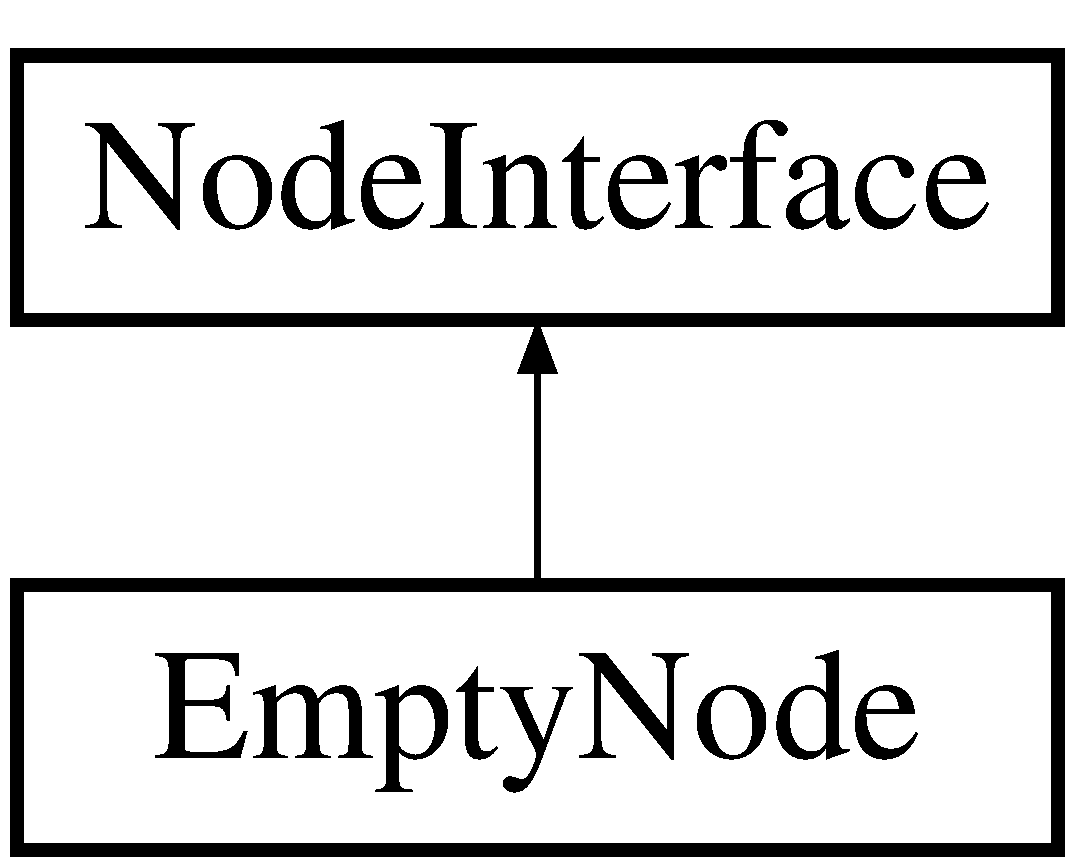
\includegraphics[height=2.000000cm]{class_empty_node}
\end{center}
\end{figure}
\subsection*{Public Member Functions}
\begin{DoxyCompactItemize}
\item 
\mbox{\Hypertarget{class_empty_node_a9e18fe1b046d001ca7b2daf87d2fd5bb}\label{class_empty_node_a9e18fe1b046d001ca7b2daf87d2fd5bb}} 
\mbox{\hyperlink{class_empty_node_a9e18fe1b046d001ca7b2daf87d2fd5bb}{Empty\+Node}} (int p\+\_\+cost)
\begin{DoxyCompactList}\small\item\em Constructor. \end{DoxyCompactList}\item 
\mbox{\hyperlink{class_empty_node_aa8c8d6db9649c4ff5624be87953092d1}{$\sim$\+Empty\+Node}} ()
\begin{DoxyCompactList}\small\item\em Deconstructor. \end{DoxyCompactList}\item 
\mbox{\Hypertarget{class_empty_node_ae11626adf3ad771cfcc68599c67ff354}\label{class_empty_node_ae11626adf3ad771cfcc68599c67ff354}} 
void \mbox{\hyperlink{class_empty_node_ae11626adf3ad771cfcc68599c67ff354}{update\+Node}} (float p\+\_\+time) override
\begin{DoxyCompactList}\small\item\em update method \end{DoxyCompactList}\item 
sf\+::\+Sprite $\ast$ \mbox{\hyperlink{class_empty_node_a1f449e50eefe1388f5b255a5dc027cc8}{get\+Sprite}} () override
\begin{DoxyCompactList}\small\item\em Gets a sprite. \end{DoxyCompactList}\item 
\mbox{\Hypertarget{class_empty_node_a50183fa0423e94904facd89bd70062f4}\label{class_empty_node_a50183fa0423e94904facd89bd70062f4}} 
void \mbox{\hyperlink{class_empty_node_a50183fa0423e94904facd89bd70062f4}{construct\+Node}} (int p\+\_\+x, int p\+\_\+y, sf\+::\+Texture p\+\_\+T) override
\begin{DoxyCompactList}\small\item\em Constructs the node. \end{DoxyCompactList}\item 
std\+::string \mbox{\hyperlink{class_empty_node_a2281f852354a5b95ba06f4e2a7e8de34}{check\+Node\+Type}} () override
\begin{DoxyCompactList}\small\item\em Method to check what type the node is. \end{DoxyCompactList}\end{DoxyCompactItemize}
\subsection*{Additional Inherited Members}


\subsection{Detailed Description}
This class is designed to be the wall, a node that should not allow the unit to move too 

\subsection{Constructor \& Destructor Documentation}
\mbox{\Hypertarget{class_empty_node_aa8c8d6db9649c4ff5624be87953092d1}\label{class_empty_node_aa8c8d6db9649c4ff5624be87953092d1}} 
\index{Empty\+Node@{Empty\+Node}!````~Empty\+Node@{$\sim$\+Empty\+Node}}
\index{````~Empty\+Node@{$\sim$\+Empty\+Node}!Empty\+Node@{Empty\+Node}}
\subsubsection{\texorpdfstring{$\sim$\+Empty\+Node()}{~EmptyNode()}}
{\footnotesize\ttfamily Empty\+Node\+::$\sim$\+Empty\+Node (\begin{DoxyParamCaption}{ }\end{DoxyParamCaption})}



Deconstructor. 


\begin{DoxyParams}{Parameters}
{\em p\+\_\+cost} & what is the cost of the node \\
\hline
\end{DoxyParams}


\subsection{Member Function Documentation}
\mbox{\Hypertarget{class_empty_node_a2281f852354a5b95ba06f4e2a7e8de34}\label{class_empty_node_a2281f852354a5b95ba06f4e2a7e8de34}} 
\index{Empty\+Node@{Empty\+Node}!check\+Node\+Type@{check\+Node\+Type}}
\index{check\+Node\+Type@{check\+Node\+Type}!Empty\+Node@{Empty\+Node}}
\subsubsection{\texorpdfstring{check\+Node\+Type()}{checkNodeType()}}
{\footnotesize\ttfamily std\+::string Empty\+Node\+::check\+Node\+Type (\begin{DoxyParamCaption}{ }\end{DoxyParamCaption})\hspace{0.3cm}{\ttfamily [override]}, {\ttfamily [virtual]}}



Method to check what type the node is. 


\begin{DoxyParams}{Parameters}
{\em p\+\_\+x} & it is the x posiiton \\
\hline
{\em p\+\_\+y} & it is the y position \\
\hline
{\em p\+\_\+T} & the texture of the node \\
\hline
\end{DoxyParams}


Implements \mbox{\hyperlink{class_node_interface_a944dbfa74de55bdef1d583f318888aeb}{Node\+Interface}}.

\mbox{\Hypertarget{class_empty_node_a1f449e50eefe1388f5b255a5dc027cc8}\label{class_empty_node_a1f449e50eefe1388f5b255a5dc027cc8}} 
\index{Empty\+Node@{Empty\+Node}!get\+Sprite@{get\+Sprite}}
\index{get\+Sprite@{get\+Sprite}!Empty\+Node@{Empty\+Node}}
\subsubsection{\texorpdfstring{get\+Sprite()}{getSprite()}}
{\footnotesize\ttfamily sf\+::\+Sprite$\ast$ Empty\+Node\+::get\+Sprite (\begin{DoxyParamCaption}{ }\end{DoxyParamCaption})\hspace{0.3cm}{\ttfamily [override]}, {\ttfamily [virtual]}}



Gets a sprite. 


\begin{DoxyParams}{Parameters}
{\em p\+\_\+time} & contains information on the time \\
\hline
\end{DoxyParams}


Implements \mbox{\hyperlink{class_node_interface_a3d79c567537e9ffa7d2fc821495879fb}{Node\+Interface}}.



The documentation for this class was generated from the following file\+:\begin{DoxyCompactItemize}
\item 
C\+:/\+Users/\+The Stormtrooper/\+Source/\+Repos/\+Final\+Year\+Project9/\+Vampires\+Vs\+Knights/include/Empty\+Node.\+h\end{DoxyCompactItemize}

\hypertarget{class_end_screen}{}\section{End\+Screen Class Reference}
\label{class_end_screen}\index{End\+Screen@{End\+Screen}}
Inheritance diagram for End\+Screen\+:\begin{figure}[H]
\begin{center}
\leavevmode
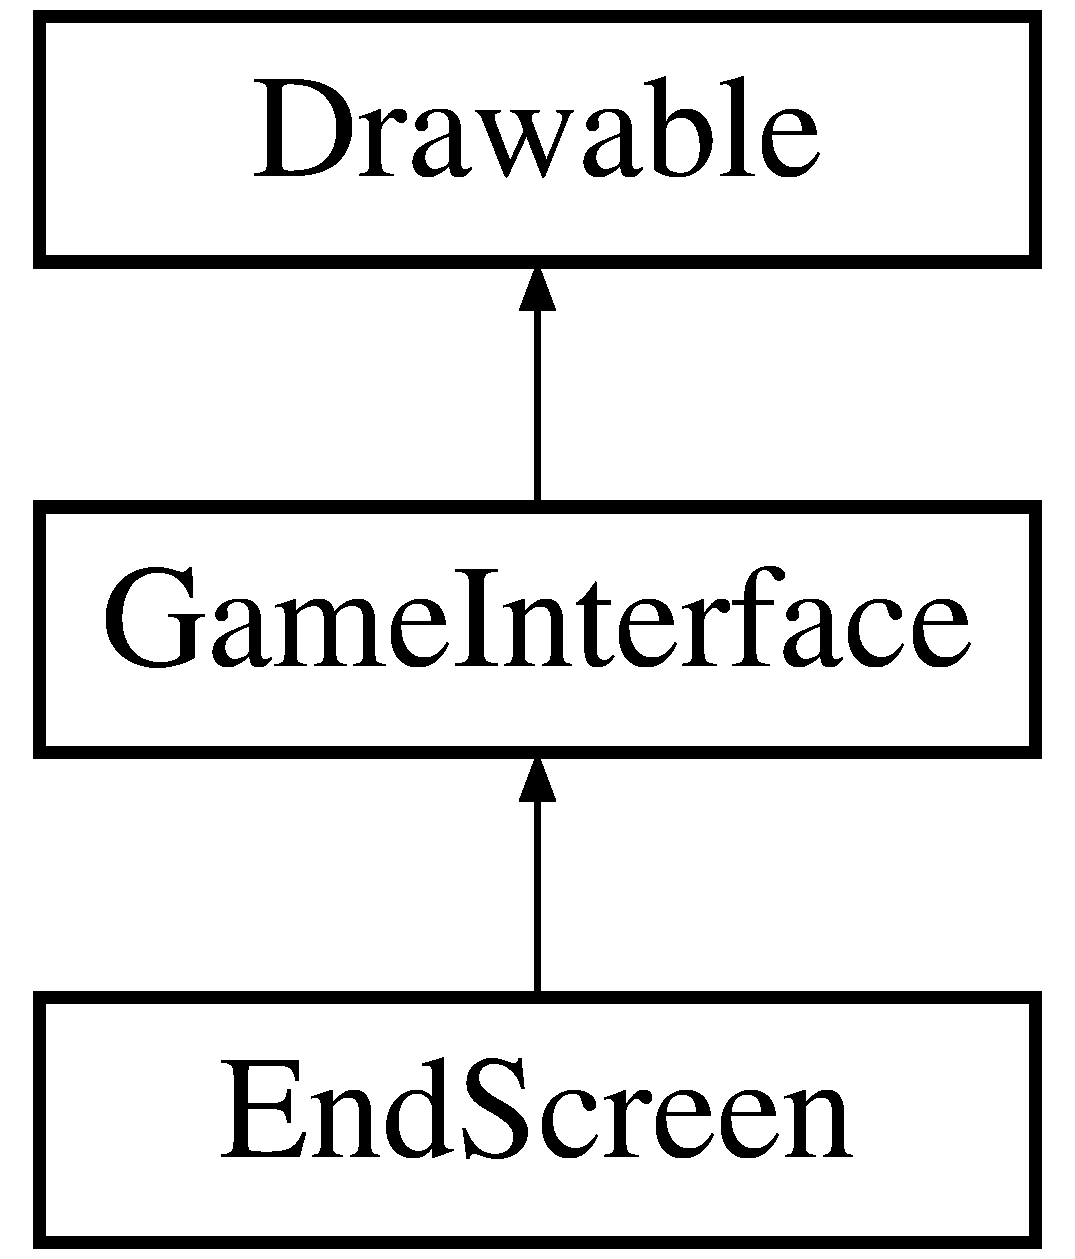
\includegraphics[height=3.000000cm]{class_end_screen}
\end{center}
\end{figure}
\subsection*{Public Member Functions}
\begin{DoxyCompactItemize}
\item 
\mbox{\Hypertarget{class_end_screen_a1da4fb23f00049e554bc5da3506248a3}\label{class_end_screen_a1da4fb23f00049e554bc5da3506248a3}} 
\mbox{\hyperlink{class_end_screen_a1da4fb23f00049e554bc5da3506248a3}{End\+Screen}} (std\+::string p\+\_\+rounds, std\+::string p\+\_\+time, std\+::string p\+\_\+text)
\begin{DoxyCompactList}\small\item\em Constructs the end screen. \end{DoxyCompactList}\item 
\mbox{\hyperlink{class_end_screen_a2bf71fd8fe94ee4ff206ff5303110864}{$\sim$\+End\+Screen}} ()
\begin{DoxyCompactList}\small\item\em Deconstructor. \end{DoxyCompactList}\item 
\mbox{\Hypertarget{class_end_screen_acd68d144cfdf319138fb301f7f005fb0}\label{class_end_screen_acd68d144cfdf319138fb301f7f005fb0}} 
void \mbox{\hyperlink{class_end_screen_acd68d144cfdf319138fb301f7f005fb0}{update\+Game}} (float p\+\_\+time) override
\begin{DoxyCompactList}\small\item\em Updates the \mbox{\hyperlink{class_end_screen}{End\+Screen}}. \end{DoxyCompactList}\item 
void \mbox{\hyperlink{class_end_screen_a7116698624a0a4af8e746c50800fe432}{draw}} (sf\+::\+Render\+Target \&target, sf\+::\+Render\+States states) const override
\begin{DoxyCompactList}\small\item\em draws the end screen \end{DoxyCompactList}\item 
void \mbox{\hyperlink{class_end_screen_a33052db95f0c2aab9e4b2e0cbeec9e8e}{handle\+Input}} (int p\+\_\+\+Input\+Event) override
\begin{DoxyCompactList}\small\item\em Handles the. \end{DoxyCompactList}\item 
virtual End\+State \mbox{\hyperlink{class_end_screen_acd13799a074bb1984352a5262c3e3f29}{is\+Over}} () override
\begin{DoxyCompactList}\small\item\em Returns the end state of the class. \end{DoxyCompactList}\item 
\mbox{\Hypertarget{class_end_screen_aaca6fd16b77f8c78f8eb0f87aa6772ff}\label{class_end_screen_aaca6fd16b77f8c78f8eb0f87aa6772ff}} 
virtual void \mbox{\hyperlink{class_end_screen_aaca6fd16b77f8c78f8eb0f87aa6772ff}{load\+Level}} () override
\begin{DoxyCompactList}\small\item\em interface demands this to be here needed in other classes \end{DoxyCompactList}\end{DoxyCompactItemize}
\subsection*{Private Attributes}
\begin{DoxyCompactItemize}
\item 
\mbox{\Hypertarget{class_end_screen_a731fe85d621665a781f5b9754f9fd8bf}\label{class_end_screen_a731fe85d621665a781f5b9754f9fd8bf}} 
\mbox{\hyperlink{class_texture_handler}{Texture\+Handler}} $\ast$ \mbox{\hyperlink{class_end_screen_a731fe85d621665a781f5b9754f9fd8bf}{m\+\_\+textures}}
\begin{DoxyCompactList}\small\item\em Gets the textures. \end{DoxyCompactList}\item 
\mbox{\Hypertarget{class_end_screen_a981ca19d838d0b2c669eb0f34a9900bc}\label{class_end_screen_a981ca19d838d0b2c669eb0f34a9900bc}} 
End\+State \mbox{\hyperlink{class_end_screen_a981ca19d838d0b2c669eb0f34a9900bc}{m\+\_\+over}}
\begin{DoxyCompactList}\small\item\em stores the end screen state \end{DoxyCompactList}\item 
\mbox{\Hypertarget{class_end_screen_a4a997b23ab2d79fe75dd7ceea33ea1ae}\label{class_end_screen_a4a997b23ab2d79fe75dd7ceea33ea1ae}} 
sf\+::\+Font \mbox{\hyperlink{class_end_screen_a4a997b23ab2d79fe75dd7ceea33ea1ae}{m\+\_\+font}}
\begin{DoxyCompactList}\small\item\em Stores the font. \end{DoxyCompactList}\item 
\mbox{\Hypertarget{class_end_screen_a1f1c5b95fd0a4956ca424b9cb648baba}\label{class_end_screen_a1f1c5b95fd0a4956ca424b9cb648baba}} 
sf\+::\+Text \mbox{\hyperlink{class_end_screen_a1f1c5b95fd0a4956ca424b9cb648baba}{m\+\_\+round\+Text}}
\begin{DoxyCompactList}\small\item\em used to display what round the player was on to the screen \end{DoxyCompactList}\item 
\mbox{\Hypertarget{class_end_screen_af88c60579eafb6a373f27e91bb9e979a}\label{class_end_screen_af88c60579eafb6a373f27e91bb9e979a}} 
sf\+::\+Text \mbox{\hyperlink{class_end_screen_af88c60579eafb6a373f27e91bb9e979a}{m\+\_\+time\+Text}}
\begin{DoxyCompactList}\small\item\em Displays the time. \end{DoxyCompactList}\item 
\mbox{\Hypertarget{class_end_screen_a63e6204ce588b54205a973d9607cb34d}\label{class_end_screen_a63e6204ce588b54205a973d9607cb34d}} 
sf\+::\+Text \mbox{\hyperlink{class_end_screen_a63e6204ce588b54205a973d9607cb34d}{m\+\_\+screen\+Text}}
\begin{DoxyCompactList}\small\item\em Displays text to the end screen. \end{DoxyCompactList}\item 
\mbox{\Hypertarget{class_end_screen_aeb22f5f583972358483e76eb0ae34e68}\label{class_end_screen_aeb22f5f583972358483e76eb0ae34e68}} 
sf\+::\+Sprite \mbox{\hyperlink{class_end_screen_aeb22f5f583972358483e76eb0ae34e68}{m\+\_\+s\+Background}}
\begin{DoxyCompactList}\small\item\em The Background sprite of the end screen. \end{DoxyCompactList}\item 
\mbox{\Hypertarget{class_end_screen_a2c4defa1110c242bef3ada6e6404d549}\label{class_end_screen_a2c4defa1110c242bef3ada6e6404d549}} 
sf\+::\+Texture \mbox{\hyperlink{class_end_screen_a2c4defa1110c242bef3ada6e6404d549}{m\+\_\+t\+Background}}
\begin{DoxyCompactList}\small\item\em Texture of the background. \end{DoxyCompactList}\end{DoxyCompactItemize}
\subsection*{Additional Inherited Members}


\subsection{Constructor \& Destructor Documentation}
\mbox{\Hypertarget{class_end_screen_a2bf71fd8fe94ee4ff206ff5303110864}\label{class_end_screen_a2bf71fd8fe94ee4ff206ff5303110864}} 
\index{End\+Screen@{End\+Screen}!````~End\+Screen@{$\sim$\+End\+Screen}}
\index{````~End\+Screen@{$\sim$\+End\+Screen}!End\+Screen@{End\+Screen}}
\subsubsection{\texorpdfstring{$\sim$\+End\+Screen()}{~EndScreen()}}
{\footnotesize\ttfamily End\+Screen\+::$\sim$\+End\+Screen (\begin{DoxyParamCaption}{ }\end{DoxyParamCaption})}



Deconstructor. 


\begin{DoxyParams}{Parameters}
{\em p\+\_\+rounds} & contains the string for text \\
\hline
{\em p\+\_\+time} & contains string text \\
\hline
{\em p\+\_\+text} & contains text to be added to the screen \\
\hline
\end{DoxyParams}


\subsection{Member Function Documentation}
\mbox{\Hypertarget{class_end_screen_a7116698624a0a4af8e746c50800fe432}\label{class_end_screen_a7116698624a0a4af8e746c50800fe432}} 
\index{End\+Screen@{End\+Screen}!draw@{draw}}
\index{draw@{draw}!End\+Screen@{End\+Screen}}
\subsubsection{\texorpdfstring{draw()}{draw()}}
{\footnotesize\ttfamily void End\+Screen\+::draw (\begin{DoxyParamCaption}\item[{sf\+::\+Render\+Target \&}]{target,  }\item[{sf\+::\+Render\+States}]{states }\end{DoxyParamCaption}) const\hspace{0.3cm}{\ttfamily [override]}, {\ttfamily [virtual]}}



draws the end screen 


\begin{DoxyParams}{Parameters}
{\em p\+\_\+time} & contains information on the time \\
\hline
\end{DoxyParams}


Implements \mbox{\hyperlink{class_game_interface_ab33712e6b22b934982896ea0cab1699a}{Game\+Interface}}.

\mbox{\Hypertarget{class_end_screen_a33052db95f0c2aab9e4b2e0cbeec9e8e}\label{class_end_screen_a33052db95f0c2aab9e4b2e0cbeec9e8e}} 
\index{End\+Screen@{End\+Screen}!handle\+Input@{handle\+Input}}
\index{handle\+Input@{handle\+Input}!End\+Screen@{End\+Screen}}
\subsubsection{\texorpdfstring{handle\+Input()}{handleInput()}}
{\footnotesize\ttfamily void End\+Screen\+::handle\+Input (\begin{DoxyParamCaption}\item[{int}]{p\+\_\+\+Input\+Event }\end{DoxyParamCaption})\hspace{0.3cm}{\ttfamily [override]}, {\ttfamily [virtual]}}



Handles the. 


\begin{DoxyParams}{Parameters}
{\em target} & draw this \\
\hline
{\em states} & paramater needed for the draw method \\
\hline
\end{DoxyParams}


Implements \mbox{\hyperlink{class_game_interface_a48b4f6059c14c79359d30b77016a28f0}{Game\+Interface}}.

\mbox{\Hypertarget{class_end_screen_acd13799a074bb1984352a5262c3e3f29}\label{class_end_screen_acd13799a074bb1984352a5262c3e3f29}} 
\index{End\+Screen@{End\+Screen}!is\+Over@{is\+Over}}
\index{is\+Over@{is\+Over}!End\+Screen@{End\+Screen}}
\subsubsection{\texorpdfstring{is\+Over()}{isOver()}}
{\footnotesize\ttfamily virtual End\+State End\+Screen\+::is\+Over (\begin{DoxyParamCaption}{ }\end{DoxyParamCaption})\hspace{0.3cm}{\ttfamily [override]}, {\ttfamily [virtual]}}



Returns the end state of the class. 


\begin{DoxyParams}{Parameters}
{\em p\+\_\+\+Input\+Event} & information needed to know what key is pressed \\
\hline
\end{DoxyParams}


Implements \mbox{\hyperlink{class_game_interface_a5bad60f237214cb1ec013e221ed16f45}{Game\+Interface}}.



The documentation for this class was generated from the following file\+:\begin{DoxyCompactItemize}
\item 
C\+:/\+Users/\+The Stormtrooper/\+Source/\+Repos/\+Final\+Year\+Project9/\+Vampires\+Vs\+Knights/include/End\+Screen.\+h\end{DoxyCompactItemize}

\hypertarget{class_file_reader}{}\section{File\+Reader Class Reference}
\label{class_file_reader}\index{File\+Reader@{File\+Reader}}


{\ttfamily \#include $<$File\+Reader.\+h$>$}

\subsection*{Public Member Functions}
\begin{DoxyCompactItemize}
\item 
\mbox{\Hypertarget{class_file_reader_a1382969e8f1468f3b04ad4b44ab39dee}\label{class_file_reader_a1382969e8f1468f3b04ad4b44ab39dee}} 
\mbox{\hyperlink{class_file_reader_a1382969e8f1468f3b04ad4b44ab39dee}{$\sim$\+File\+Reader}} ()
\begin{DoxyCompactList}\small\item\em Deconstructor. \end{DoxyCompactList}\item 
\mbox{\Hypertarget{class_file_reader_a746a2d82fb15782f219cb38fa5bd643a}\label{class_file_reader_a746a2d82fb15782f219cb38fa5bd643a}} 
\mbox{\hyperlink{class_file_reader_a746a2d82fb15782f219cb38fa5bd643a}{File\+Reader}} (std\+::string p\+\_\+level)
\begin{DoxyCompactList}\small\item\em Constructor the File counts as its own object. \end{DoxyCompactList}\item 
std\+::vector$<$ float $>$ \mbox{\hyperlink{class_file_reader_ae3af120919f987fec28d577d9e67a7d6}{get\+Speed\+Values}} ()
\begin{DoxyCompactList}\small\item\em a get method that returns a vector of floats used to give characters their speed value \end{DoxyCompactList}\item 
\mbox{\Hypertarget{class_file_reader_aed6a77a700fd3e5201dc13535833e50f}\label{class_file_reader_aed6a77a700fd3e5201dc13535833e50f}} 
std\+::vector$<$ sf\+::\+Vector2i $>$ \mbox{\hyperlink{class_file_reader_aed6a77a700fd3e5201dc13535833e50f}{get\+Positions}} ()
\begin{DoxyCompactList}\small\item\em used to get all the characters positions within the grid \end{DoxyCompactList}\item 
\mbox{\Hypertarget{class_file_reader_a6bc93c7b23eddf37b5be069a954ed0d9}\label{class_file_reader_a6bc93c7b23eddf37b5be069a954ed0d9}} 
std\+::vector$<$ float $>$ \mbox{\hyperlink{class_file_reader_a6bc93c7b23eddf37b5be069a954ed0d9}{get\+Health}} ()
\begin{DoxyCompactList}\small\item\em gets all the characters health\textquotesingle{}s \end{DoxyCompactList}\item 
\mbox{\Hypertarget{class_file_reader_af5057b4e395f53fd8fdbc50d52c21605}\label{class_file_reader_af5057b4e395f53fd8fdbc50d52c21605}} 
std\+::vector$<$ float $>$ \mbox{\hyperlink{class_file_reader_af5057b4e395f53fd8fdbc50d52c21605}{get\+Attack}} ()
\begin{DoxyCompactList}\small\item\em gets all the characaters attack stats \end{DoxyCompactList}\item 
\mbox{\Hypertarget{class_file_reader_ae527378ff9f7cae400c526d2580149cd}\label{class_file_reader_ae527378ff9f7cae400c526d2580149cd}} 
std\+::vector$<$ std\+::string $>$ \mbox{\hyperlink{class_file_reader_ae527378ff9f7cae400c526d2580149cd}{get\+Texture}} ()
\begin{DoxyCompactList}\small\item\em This tells the character what its texture is. \end{DoxyCompactList}\item 
\mbox{\Hypertarget{class_file_reader_a8e7d0a24c23871079074ee522f904401}\label{class_file_reader_a8e7d0a24c23871079074ee522f904401}} 
int \mbox{\hyperlink{class_file_reader_a8e7d0a24c23871079074ee522f904401}{get\+Start\+Of\+Vamps}} ()
\begin{DoxyCompactList}\small\item\em tells the scene when the vampires start in the vector \end{DoxyCompactList}\end{DoxyCompactItemize}
\subsection*{Protected Attributes}
\begin{DoxyCompactItemize}
\item 
\mbox{\Hypertarget{class_file_reader_a5a8ec51093ebc6e21a82a151e0672375}\label{class_file_reader_a5a8ec51093ebc6e21a82a151e0672375}} 
std\+::vector$<$ float $>$ \mbox{\hyperlink{class_file_reader_a5a8ec51093ebc6e21a82a151e0672375}{m\+\_\+speed\+Values}}
\begin{DoxyCompactList}\small\item\em stores the speed values \end{DoxyCompactList}\item 
\mbox{\Hypertarget{class_file_reader_a1987e0f71700746437cee5b9231d5cfe}\label{class_file_reader_a1987e0f71700746437cee5b9231d5cfe}} 
std\+::vector$<$ sf\+::\+Vector2i $>$ \mbox{\hyperlink{class_file_reader_a1987e0f71700746437cee5b9231d5cfe}{m\+\_\+\+Positions}}
\begin{DoxyCompactList}\small\item\em stores the positions \end{DoxyCompactList}\item 
\mbox{\Hypertarget{class_file_reader_a4fc27357cabaa49c75dcb2d07617e4d4}\label{class_file_reader_a4fc27357cabaa49c75dcb2d07617e4d4}} 
std\+::vector$<$ float $>$ \mbox{\hyperlink{class_file_reader_a4fc27357cabaa49c75dcb2d07617e4d4}{m\+\_\+health}}
\begin{DoxyCompactList}\small\item\em stores health \end{DoxyCompactList}\item 
\mbox{\Hypertarget{class_file_reader_a48a65dfc7c279d5e5773f2bdf7a40f5c}\label{class_file_reader_a48a65dfc7c279d5e5773f2bdf7a40f5c}} 
std\+::vector$<$ float $>$ \mbox{\hyperlink{class_file_reader_a48a65dfc7c279d5e5773f2bdf7a40f5c}{m\+\_\+attack}}
\begin{DoxyCompactList}\small\item\em stores attack \end{DoxyCompactList}\item 
\mbox{\Hypertarget{class_file_reader_a7579fb5818df13d3f241bf22e46502b3}\label{class_file_reader_a7579fb5818df13d3f241bf22e46502b3}} 
std\+::vector$<$ std\+::string $>$ \mbox{\hyperlink{class_file_reader_a7579fb5818df13d3f241bf22e46502b3}{m\+\_\+texture}}
\begin{DoxyCompactList}\small\item\em stores texture id \end{DoxyCompactList}\item 
\mbox{\Hypertarget{class_file_reader_ad5eb0b8736cea57b3823f50d8bf4929a}\label{class_file_reader_ad5eb0b8736cea57b3823f50d8bf4929a}} 
int \mbox{\hyperlink{class_file_reader_ad5eb0b8736cea57b3823f50d8bf4929a}{m\+\_\+start\+Of\+Vampires}}
\begin{DoxyCompactList}\small\item\em stores an int used for to determine when the vampires start in a vector \end{DoxyCompactList}\end{DoxyCompactItemize}


\subsection{Detailed Description}
File Reader that is used to load in characters and there stats 

\subsection{Member Function Documentation}
\mbox{\Hypertarget{class_file_reader_ae3af120919f987fec28d577d9e67a7d6}\label{class_file_reader_ae3af120919f987fec28d577d9e67a7d6}} 
\index{File\+Reader@{File\+Reader}!get\+Speed\+Values@{get\+Speed\+Values}}
\index{get\+Speed\+Values@{get\+Speed\+Values}!File\+Reader@{File\+Reader}}
\subsubsection{\texorpdfstring{get\+Speed\+Values()}{getSpeedValues()}}
{\footnotesize\ttfamily std\+::vector$<$float$>$ File\+Reader\+::get\+Speed\+Values (\begin{DoxyParamCaption}{ }\end{DoxyParamCaption})}



a get method that returns a vector of floats used to give characters their speed value 


\begin{DoxyParams}{Parameters}
{\em p\+\_\+level} & dt used to tell the change in time \\
\hline
\end{DoxyParams}


The documentation for this class was generated from the following file\+:\begin{DoxyCompactItemize}
\item 
C\+:/\+Users/\+The Stormtrooper/\+Source/\+Repos/\+Final\+Year\+Project9/\+Vampires\+Vs\+Knights/include/File\+Reader.\+h\end{DoxyCompactItemize}

\hypertarget{class_file_reader_game_assests}{}\section{File\+Reader\+Game\+Assests Class Reference}
\label{class_file_reader_game_assests}\index{File\+Reader\+Game\+Assests@{File\+Reader\+Game\+Assests}}


{\ttfamily \#include $<$File\+Reader\+Game\+Assests.\+h$>$}

\subsection*{Public Member Functions}
\begin{DoxyCompactItemize}
\item 
\mbox{\Hypertarget{class_file_reader_game_assests_ab30bee0c946988ceaa3e9ba6f8ecf190}\label{class_file_reader_game_assests_ab30bee0c946988ceaa3e9ba6f8ecf190}} 
\mbox{\hyperlink{class_file_reader_game_assests_ab30bee0c946988ceaa3e9ba6f8ecf190}{File\+Reader\+Game\+Assests}} (std\+::string p\+\_\+\+Textures, std\+::string p\+\_\+\+Levels)
\begin{DoxyCompactList}\small\item\em Constructor for the class. \end{DoxyCompactList}\item 
std\+::vector$<$ std\+::pair$<$ std\+::string, std\+::string $>$ $>$ \mbox{\hyperlink{class_file_reader_game_assests_a952fd5fb0c4d71319af28483ef60ad84}{get\+Textures}} ()
\begin{DoxyCompactList}\small\item\em a vector of a pair of strings that gets all the containing all the texture information \end{DoxyCompactList}\item 
\mbox{\Hypertarget{class_file_reader_game_assests_a3d89ce1322e0bfe0c104a055d662deac}\label{class_file_reader_game_assests_a3d89ce1322e0bfe0c104a055d662deac}} 
std\+::vector$<$ std\+::pair$<$ std\+::string, std\+::string $>$ $>$ \mbox{\hyperlink{class_file_reader_game_assests_a3d89ce1322e0bfe0c104a055d662deac}{get\+Levels}} ()
\begin{DoxyCompactList}\small\item\em a vector of a pair of strings which get level information inside of them \end{DoxyCompactList}\end{DoxyCompactItemize}
\subsection*{Private Attributes}
\begin{DoxyCompactItemize}
\item 
\mbox{\Hypertarget{class_file_reader_game_assests_a4be62add5fcf98f1bd551e8d4c8ab34c}\label{class_file_reader_game_assests_a4be62add5fcf98f1bd551e8d4c8ab34c}} 
std\+::vector$<$ std\+::pair$<$ std\+::string, std\+::string $>$ $>$ \mbox{\hyperlink{class_file_reader_game_assests_a4be62add5fcf98f1bd551e8d4c8ab34c}{m\+\_\+\+Textures}}
\begin{DoxyCompactList}\small\item\em stores a vector of textures \end{DoxyCompactList}\item 
\mbox{\Hypertarget{class_file_reader_game_assests_ab160d574a819bfe608fef64fc20b6bad}\label{class_file_reader_game_assests_ab160d574a819bfe608fef64fc20b6bad}} 
std\+::vector$<$ std\+::pair$<$ std\+::string, std\+::string $>$ $>$ \mbox{\hyperlink{class_file_reader_game_assests_ab160d574a819bfe608fef64fc20b6bad}{m\+\_\+\+Levels}}
\begin{DoxyCompactList}\small\item\em stores a vector of levels \end{DoxyCompactList}\end{DoxyCompactItemize}


\subsection{Detailed Description}
Another file reader with the purpose of loading in textures and levels 

\subsection{Member Function Documentation}
\mbox{\Hypertarget{class_file_reader_game_assests_a952fd5fb0c4d71319af28483ef60ad84}\label{class_file_reader_game_assests_a952fd5fb0c4d71319af28483ef60ad84}} 
\index{File\+Reader\+Game\+Assests@{File\+Reader\+Game\+Assests}!get\+Textures@{get\+Textures}}
\index{get\+Textures@{get\+Textures}!File\+Reader\+Game\+Assests@{File\+Reader\+Game\+Assests}}
\subsubsection{\texorpdfstring{get\+Textures()}{getTextures()}}
{\footnotesize\ttfamily std\+::vector$<$std\+::pair$<$std\+::string, std\+::string$>$ $>$ File\+Reader\+Game\+Assests\+::get\+Textures (\begin{DoxyParamCaption}{ }\end{DoxyParamCaption})}



a vector of a pair of strings that gets all the containing all the texture information 


\begin{DoxyParams}{Parameters}
{\em p\+\_\+\+Textures} & string containing information on where to find the texture file \\
\hline
{\em p\+\_\+\+Levels} & another string that when read gives data from the levels file \\
\hline
\end{DoxyParams}


The documentation for this class was generated from the following file\+:\begin{DoxyCompactItemize}
\item 
C\+:/\+Users/\+The Stormtrooper/\+Source/\+Repos/\+Final\+Year\+Project9/\+Vampires\+Vs\+Knights/include/File\+Reader\+Game\+Assests.\+h\end{DoxyCompactItemize}

\hypertarget{class_file_reader_nodes}{}\section{File\+Reader\+Nodes Class Reference}
\label{class_file_reader_nodes}\index{File\+Reader\+Nodes@{File\+Reader\+Nodes}}


{\ttfamily \#include $<$File\+Reader\+Nodes.\+h$>$}

\subsection*{Public Member Functions}
\begin{DoxyCompactItemize}
\item 
\mbox{\Hypertarget{class_file_reader_nodes_ac6a6baa2a1d62b201db74cd288ce40eb}\label{class_file_reader_nodes_ac6a6baa2a1d62b201db74cd288ce40eb}} 
\mbox{\hyperlink{class_file_reader_nodes_ac6a6baa2a1d62b201db74cd288ce40eb}{File\+Reader\+Nodes}} (std\+::string p\+\_\+\+Nodes)
\begin{DoxyCompactList}\small\item\em Constructs the file loader for the nodes. \end{DoxyCompactList}\item 
std\+::vector$<$ sf\+::\+Vector2i $>$ \mbox{\hyperlink{class_file_reader_nodes_a87231f197c15e2ef9e81e27cc9055276}{get\+Node\+ID}} ()
\begin{DoxyCompactList}\small\item\em Gets the positions of the node. \end{DoxyCompactList}\item 
\mbox{\Hypertarget{class_file_reader_nodes_a1277ad182dbc6544fe60556930c517dc}\label{class_file_reader_nodes_a1277ad182dbc6544fe60556930c517dc}} 
std\+::vector$<$ std\+::string $>$ \mbox{\hyperlink{class_file_reader_nodes_a1277ad182dbc6544fe60556930c517dc}{get\+Node\+Types}} ()
\begin{DoxyCompactList}\small\item\em Gets a string each with a node type. \end{DoxyCompactList}\item 
\mbox{\Hypertarget{class_file_reader_nodes_ae75b4dd1ba8287ad904c94068f6922c2}\label{class_file_reader_nodes_ae75b4dd1ba8287ad904c94068f6922c2}} 
std\+::vector$<$ float $>$ \mbox{\hyperlink{class_file_reader_nodes_ae75b4dd1ba8287ad904c94068f6922c2}{get\+Cost}} ()
\begin{DoxyCompactList}\small\item\em Gets the cost of moving over the node. \end{DoxyCompactList}\end{DoxyCompactItemize}
\subsection*{Private Attributes}
\begin{DoxyCompactItemize}
\item 
\mbox{\Hypertarget{class_file_reader_nodes_ac85d20778aba56dfed18856d1ebec542}\label{class_file_reader_nodes_ac85d20778aba56dfed18856d1ebec542}} 
std\+::vector$<$ sf\+::\+Vector2i $>$ \mbox{\hyperlink{class_file_reader_nodes_ac85d20778aba56dfed18856d1ebec542}{m\+\_\+node\+ID}}
\begin{DoxyCompactList}\small\item\em Stores the nodes position. \end{DoxyCompactList}\item 
\mbox{\Hypertarget{class_file_reader_nodes_ab07771dd9275e0c9e94a3db3d230d68b}\label{class_file_reader_nodes_ab07771dd9275e0c9e94a3db3d230d68b}} 
std\+::vector$<$ std\+::string $>$ \mbox{\hyperlink{class_file_reader_nodes_ab07771dd9275e0c9e94a3db3d230d68b}{m\+\_\+node\+Types}}
\begin{DoxyCompactList}\small\item\em Stores the nodes types. \end{DoxyCompactList}\item 
\mbox{\Hypertarget{class_file_reader_nodes_a9aa3c874c878bf68bf387e3a54984253}\label{class_file_reader_nodes_a9aa3c874c878bf68bf387e3a54984253}} 
std\+::vector$<$ float $>$ \mbox{\hyperlink{class_file_reader_nodes_a9aa3c874c878bf68bf387e3a54984253}{m\+\_\+cost}}
\begin{DoxyCompactList}\small\item\em stores the cost for moving over the node \end{DoxyCompactList}\end{DoxyCompactItemize}


\subsection{Detailed Description}
Another file that stores what nodes are going to be put into the game 

\subsection{Member Function Documentation}
\mbox{\Hypertarget{class_file_reader_nodes_a87231f197c15e2ef9e81e27cc9055276}\label{class_file_reader_nodes_a87231f197c15e2ef9e81e27cc9055276}} 
\index{File\+Reader\+Nodes@{File\+Reader\+Nodes}!get\+Node\+ID@{get\+Node\+ID}}
\index{get\+Node\+ID@{get\+Node\+ID}!File\+Reader\+Nodes@{File\+Reader\+Nodes}}
\subsubsection{\texorpdfstring{get\+Node\+I\+D()}{getNodeID()}}
{\footnotesize\ttfamily std\+::vector$<$sf\+::\+Vector2i$>$ File\+Reader\+Nodes\+::get\+Node\+ID (\begin{DoxyParamCaption}{ }\end{DoxyParamCaption})}



Gets the positions of the node. 


\begin{DoxyParams}{Parameters}
{\em p\+\_\+\+Nodes} & gets passed in a string with information on the nodes \\
\hline
\end{DoxyParams}


The documentation for this class was generated from the following file\+:\begin{DoxyCompactItemize}
\item 
C\+:/\+Users/\+The Stormtrooper/\+Source/\+Repos/\+Final\+Year\+Project9/\+Vampires\+Vs\+Knights/include/File\+Reader\+Nodes.\+h\end{DoxyCompactItemize}

\hypertarget{class_game_interface}{}\section{Game\+Interface Class Reference}
\label{class_game_interface}\index{Game\+Interface@{Game\+Interface}}


{\ttfamily \#include $<$Game\+Interface.\+h$>$}

Inheritance diagram for Game\+Interface\+:\begin{figure}[H]
\begin{center}
\leavevmode
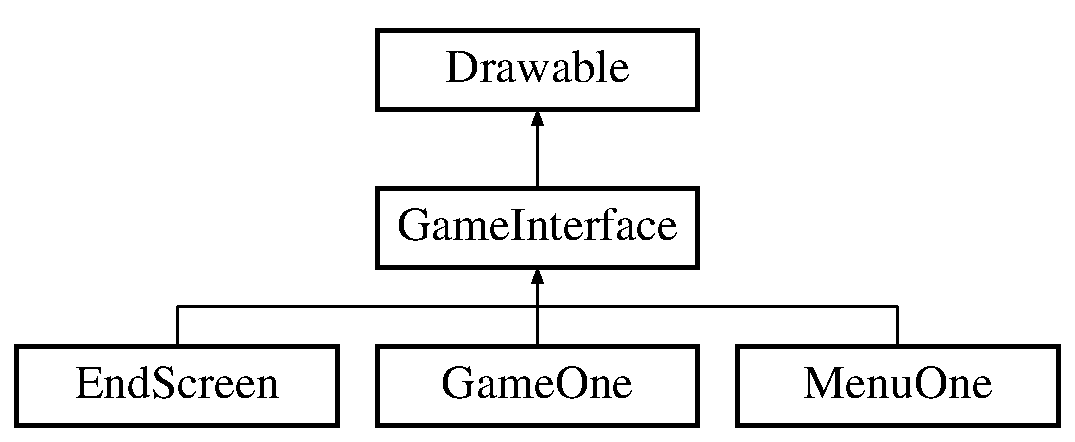
\includegraphics[height=3.000000cm]{class_game_interface}
\end{center}
\end{figure}
\subsection*{Protected Member Functions}
\begin{DoxyCompactItemize}
\item 
\mbox{\Hypertarget{class_game_interface_a5704fbd5713a20e95032dcf1631bdd67}\label{class_game_interface_a5704fbd5713a20e95032dcf1631bdd67}} 
virtual void \mbox{\hyperlink{class_game_interface_a5704fbd5713a20e95032dcf1631bdd67}{update\+Game}} (float p\+\_\+time)=0
\begin{DoxyCompactList}\small\item\em Every game needs to be updated. \end{DoxyCompactList}\item 
virtual void \mbox{\hyperlink{class_game_interface_ab33712e6b22b934982896ea0cab1699a}{draw}} (sf\+::\+Render\+Target \&target, sf\+::\+Render\+States states) const =0
\begin{DoxyCompactList}\small\item\em Every game needs to be drawn. \end{DoxyCompactList}\item 
virtual void \mbox{\hyperlink{class_game_interface_a48b4f6059c14c79359d30b77016a28f0}{handle\+Input}} (int p\+\_\+\+Input\+Event)=0
\begin{DoxyCompactList}\small\item\em Every game needs key inputs. \end{DoxyCompactList}\item 
virtual End\+State \mbox{\hyperlink{class_game_interface_a5bad60f237214cb1ec013e221ed16f45}{is\+Over}} ()=0
\begin{DoxyCompactList}\small\item\em Every game needs an end state. \end{DoxyCompactList}\item 
\mbox{\Hypertarget{class_game_interface_a48c841b894ea37938996e3d5a40353b5}\label{class_game_interface_a48c841b894ea37938996e3d5a40353b5}} 
virtual void \mbox{\hyperlink{class_game_interface_a48c841b894ea37938996e3d5a40353b5}{load\+Level}} ()=0
\begin{DoxyCompactList}\small\item\em Every game needs to be loaded. \end{DoxyCompactList}\end{DoxyCompactItemize}


\subsection{Detailed Description}
An interface class used for each window origanlly ment to be just for the game but it had values the menu\textquotesingle{}s could use 

\subsection{Member Function Documentation}
\mbox{\Hypertarget{class_game_interface_ab33712e6b22b934982896ea0cab1699a}\label{class_game_interface_ab33712e6b22b934982896ea0cab1699a}} 
\index{Game\+Interface@{Game\+Interface}!draw@{draw}}
\index{draw@{draw}!Game\+Interface@{Game\+Interface}}
\subsubsection{\texorpdfstring{draw()}{draw()}}
{\footnotesize\ttfamily virtual void Game\+Interface\+::draw (\begin{DoxyParamCaption}\item[{sf\+::\+Render\+Target \&}]{target,  }\item[{sf\+::\+Render\+States}]{states }\end{DoxyParamCaption}) const\hspace{0.3cm}{\ttfamily [protected]}, {\ttfamily [pure virtual]}}



Every game needs to be drawn. 


\begin{DoxyParams}{Parameters}
{\em p\+\_\+time} & contains information on the time \\
\hline
\end{DoxyParams}


Implemented in \mbox{\hyperlink{class_game_one_af4df2785640103b623be240fa8be1e8a}{Game\+One}}, \mbox{\hyperlink{class_end_screen_a7116698624a0a4af8e746c50800fe432}{End\+Screen}}, and \mbox{\hyperlink{class_menu_one_a861529b6fcc30daebc753186714e3cc9}{Menu\+One}}.

\mbox{\Hypertarget{class_game_interface_a48b4f6059c14c79359d30b77016a28f0}\label{class_game_interface_a48b4f6059c14c79359d30b77016a28f0}} 
\index{Game\+Interface@{Game\+Interface}!handle\+Input@{handle\+Input}}
\index{handle\+Input@{handle\+Input}!Game\+Interface@{Game\+Interface}}
\subsubsection{\texorpdfstring{handle\+Input()}{handleInput()}}
{\footnotesize\ttfamily virtual void Game\+Interface\+::handle\+Input (\begin{DoxyParamCaption}\item[{int}]{p\+\_\+\+Input\+Event }\end{DoxyParamCaption})\hspace{0.3cm}{\ttfamily [protected]}, {\ttfamily [pure virtual]}}



Every game needs key inputs. 


\begin{DoxyParams}{Parameters}
{\em target} & draw this \\
\hline
{\em states} & paramater needed for the draw method \\
\hline
\end{DoxyParams}


Implemented in \mbox{\hyperlink{class_game_one_ae1ecd54039b4a3650f0d113ef4629da3}{Game\+One}}, \mbox{\hyperlink{class_end_screen_a33052db95f0c2aab9e4b2e0cbeec9e8e}{End\+Screen}}, and \mbox{\hyperlink{class_menu_one_aee28812124909d8734eeeaecfde35f0f}{Menu\+One}}.

\mbox{\Hypertarget{class_game_interface_a5bad60f237214cb1ec013e221ed16f45}\label{class_game_interface_a5bad60f237214cb1ec013e221ed16f45}} 
\index{Game\+Interface@{Game\+Interface}!is\+Over@{is\+Over}}
\index{is\+Over@{is\+Over}!Game\+Interface@{Game\+Interface}}
\subsubsection{\texorpdfstring{is\+Over()}{isOver()}}
{\footnotesize\ttfamily virtual End\+State Game\+Interface\+::is\+Over (\begin{DoxyParamCaption}{ }\end{DoxyParamCaption})\hspace{0.3cm}{\ttfamily [protected]}, {\ttfamily [pure virtual]}}



Every game needs an end state. 


\begin{DoxyParams}{Parameters}
{\em p\+\_\+\+Input\+Event} & information needed to know what key is pressed \\
\hline
\end{DoxyParams}


Implemented in \mbox{\hyperlink{class_game_one_a9e9050de230336fac769ab5e8b23f7f8}{Game\+One}}, \mbox{\hyperlink{class_end_screen_acd13799a074bb1984352a5262c3e3f29}{End\+Screen}}, and \mbox{\hyperlink{class_menu_one_aa1d50806994903b77d44d241d7755404}{Menu\+One}}.



The documentation for this class was generated from the following file\+:\begin{DoxyCompactItemize}
\item 
C\+:/\+Users/\+The Stormtrooper/\+Source/\+Repos/\+Final\+Year\+Project9/\+Vampires\+Vs\+Knights/include/Game\+Interface.\+h\end{DoxyCompactItemize}

\hypertarget{class_game_one}{}\section{Game\+One Class Reference}
\label{class_game_one}\index{Game\+One@{Game\+One}}


{\ttfamily \#include $<$Game\+One.\+h$>$}

Inheritance diagram for Game\+One\+:\begin{figure}[H]
\begin{center}
\leavevmode
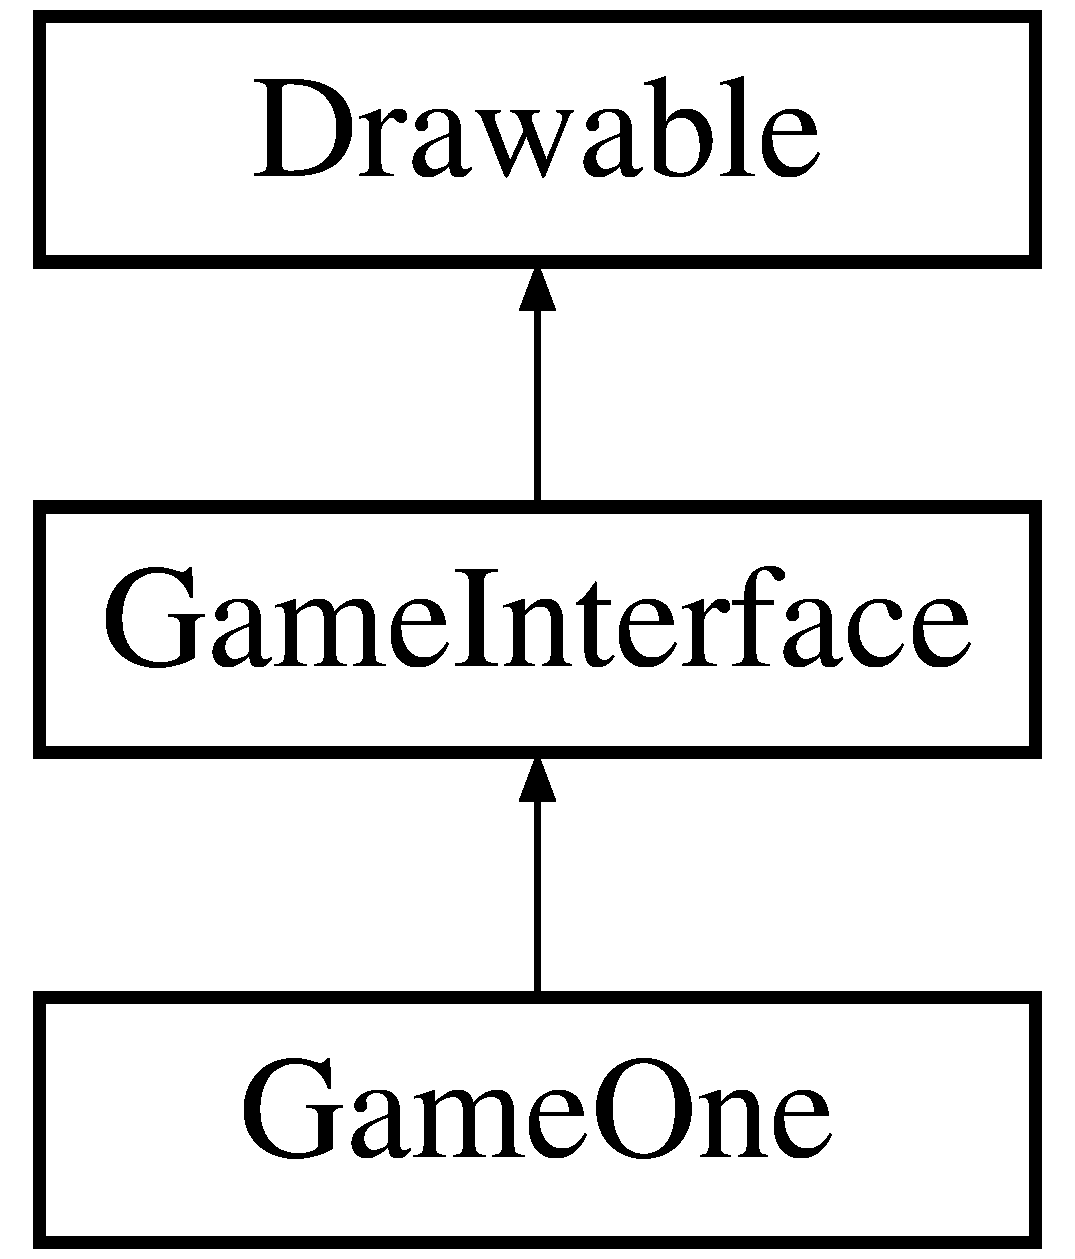
\includegraphics[height=3.000000cm]{class_game_one}
\end{center}
\end{figure}
\subsection*{Public Member Functions}
\begin{DoxyCompactItemize}
\item 
\mbox{\Hypertarget{class_game_one_aa7870529dfdb7ed178dbf2fc00a80f1e}\label{class_game_one_aa7870529dfdb7ed178dbf2fc00a80f1e}} 
\mbox{\hyperlink{class_game_one_aa7870529dfdb7ed178dbf2fc00a80f1e}{Game\+One}} (int p\+\_\+level)
\begin{DoxyCompactList}\small\item\em Constructor. \end{DoxyCompactList}\item 
\mbox{\hyperlink{class_game_one_a216b9c400f6e70b7fb6814e8b96d1cc9}{$\sim$\+Game\+One}} ()
\begin{DoxyCompactList}\small\item\em Deconstructor. \end{DoxyCompactList}\item 
\mbox{\Hypertarget{class_game_one_abb235d1a7d7415707bf07389e91f6296}\label{class_game_one_abb235d1a7d7415707bf07389e91f6296}} 
void \mbox{\hyperlink{class_game_one_abb235d1a7d7415707bf07389e91f6296}{update\+Game}} (float p\+\_\+time) override
\begin{DoxyCompactList}\small\item\em updates the game \end{DoxyCompactList}\item 
\mbox{\Hypertarget{class_game_one_af4df2785640103b623be240fa8be1e8a}\label{class_game_one_af4df2785640103b623be240fa8be1e8a}} 
void \mbox{\hyperlink{class_game_one_af4df2785640103b623be240fa8be1e8a}{draw}} (sf\+::\+Render\+Target \&target, sf\+::\+Render\+States states) const override
\begin{DoxyCompactList}\small\item\em draw game \end{DoxyCompactList}\item 
void \mbox{\hyperlink{class_game_one_ae1ecd54039b4a3650f0d113ef4629da3}{handle\+Input}} (int p\+\_\+\+Input\+Event) override
\begin{DoxyCompactList}\small\item\em Handles the inputs of the game. \end{DoxyCompactList}\item 
End\+State \mbox{\hyperlink{class_game_one_a9e9050de230336fac769ab5e8b23f7f8}{is\+Over}} () override
\begin{DoxyCompactList}\small\item\em What state is the end state. \end{DoxyCompactList}\item 
\mbox{\Hypertarget{class_game_one_ac8a6b9bdcd077157106d79f79310f057}\label{class_game_one_ac8a6b9bdcd077157106d79f79310f057}} 
void \mbox{\hyperlink{class_game_one_ac8a6b9bdcd077157106d79f79310f057}{load\+Level}} () override
\begin{DoxyCompactList}\small\item\em load the level \end{DoxyCompactList}\item 
\mbox{\Hypertarget{class_game_one_a681cbdadb061d7713f323dea331e5a31}\label{class_game_one_a681cbdadb061d7713f323dea331e5a31}} 
\mbox{\hyperlink{class_scene}{Scene}} $\ast$ \mbox{\hyperlink{class_game_one_a681cbdadb061d7713f323dea331e5a31}{get\+Scene}} ()
\begin{DoxyCompactList}\small\item\em get the scene \end{DoxyCompactList}\end{DoxyCompactItemize}
\subsection*{Private Attributes}
\begin{DoxyCompactItemize}
\item 
\mbox{\Hypertarget{class_game_one_a5072e2a0c8f6161dd2f34a8ad643760e}\label{class_game_one_a5072e2a0c8f6161dd2f34a8ad643760e}} 
\mbox{\hyperlink{class_file_reader_game_assests}{File\+Reader\+Game\+Assests}} $\ast$ \mbox{\hyperlink{class_game_one_a5072e2a0c8f6161dd2f34a8ad643760e}{m\+\_\+reader}}
\begin{DoxyCompactList}\small\item\em Used to load in game assessts. \end{DoxyCompactList}\item 
\mbox{\Hypertarget{class_game_one_a8e393ac3370d069b3996f56a8c47ff33}\label{class_game_one_a8e393ac3370d069b3996f56a8c47ff33}} 
\mbox{\hyperlink{class_scene}{Scene}} $\ast$ \mbox{\hyperlink{class_game_one_a8e393ac3370d069b3996f56a8c47ff33}{m\+\_\+current\+Scene}}
\begin{DoxyCompactList}\small\item\em Current scene of the game. \end{DoxyCompactList}\item 
\mbox{\Hypertarget{class_game_one_ac12bf28dc852ca8ef0628ba98d7d3a4e}\label{class_game_one_ac12bf28dc852ca8ef0628ba98d7d3a4e}} 
\mbox{\hyperlink{class_texture_handler}{Texture\+Handler}} $\ast$ \mbox{\hyperlink{class_game_one_ac12bf28dc852ca8ef0628ba98d7d3a4e}{m\+\_\+texture\+Handler}}
\begin{DoxyCompactList}\small\item\em handles the textures \end{DoxyCompactList}\item 
\mbox{\Hypertarget{class_game_one_a810562b54953c069d2e1dbc64d8f5421}\label{class_game_one_a810562b54953c069d2e1dbc64d8f5421}} 
sf\+::\+Sprite \mbox{\hyperlink{class_game_one_a810562b54953c069d2e1dbc64d8f5421}{m\+\_\+background\+Sprite}}
\begin{DoxyCompactList}\small\item\em The Background sprite. \end{DoxyCompactList}\item 
\mbox{\Hypertarget{class_game_one_a983b97428e90b5e77947b5dca0b3f59a}\label{class_game_one_a983b97428e90b5e77947b5dca0b3f59a}} 
sf\+::\+Texture \mbox{\hyperlink{class_game_one_a983b97428e90b5e77947b5dca0b3f59a}{m\+\_\+background\+Texture}}
\begin{DoxyCompactList}\small\item\em Background texture. \end{DoxyCompactList}\item 
\mbox{\Hypertarget{class_game_one_ac5334da542d1e258cf355452744a2d90}\label{class_game_one_ac5334da542d1e258cf355452744a2d90}} 
std\+::vector$<$ std\+::pair$<$ std\+::string, std\+::string $>$ $>$ \mbox{\hyperlink{class_game_one_ac5334da542d1e258cf355452744a2d90}{m\+\_\+vector\+Levels}}
\begin{DoxyCompactList}\small\item\em Stores the games level. \end{DoxyCompactList}\item 
\mbox{\Hypertarget{class_game_one_adaa91f89bc0a1485c8820ba000b81e53}\label{class_game_one_adaa91f89bc0a1485c8820ba000b81e53}} 
End\+State \mbox{\hyperlink{class_game_one_adaa91f89bc0a1485c8820ba000b81e53}{m\+\_\+end\+State}}
\begin{DoxyCompactList}\small\item\em Stores the end game state. \end{DoxyCompactList}\item 
\mbox{\Hypertarget{class_game_one_a6cdca32ede803a28dcad770826af33a3}\label{class_game_one_a6cdca32ede803a28dcad770826af33a3}} 
int \mbox{\hyperlink{class_game_one_a6cdca32ede803a28dcad770826af33a3}{m\+\_\+\+Level}}
\begin{DoxyCompactList}\small\item\em What level is the game currently on. \end{DoxyCompactList}\end{DoxyCompactItemize}
\subsection*{Additional Inherited Members}


\subsection{Detailed Description}
This class is is to run the game 

\subsection{Constructor \& Destructor Documentation}
\mbox{\Hypertarget{class_game_one_a216b9c400f6e70b7fb6814e8b96d1cc9}\label{class_game_one_a216b9c400f6e70b7fb6814e8b96d1cc9}} 
\index{Game\+One@{Game\+One}!````~Game\+One@{$\sim$\+Game\+One}}
\index{````~Game\+One@{$\sim$\+Game\+One}!Game\+One@{Game\+One}}
\subsubsection{\texorpdfstring{$\sim$\+Game\+One()}{~GameOne()}}
{\footnotesize\ttfamily Game\+One\+::$\sim$\+Game\+One (\begin{DoxyParamCaption}{ }\end{DoxyParamCaption})}



Deconstructor. 


\begin{DoxyParams}{Parameters}
{\em p\+\_\+level} & passes in what level should be loaded \\
\hline
\end{DoxyParams}


\subsection{Member Function Documentation}
\mbox{\Hypertarget{class_game_one_ae1ecd54039b4a3650f0d113ef4629da3}\label{class_game_one_ae1ecd54039b4a3650f0d113ef4629da3}} 
\index{Game\+One@{Game\+One}!handle\+Input@{handle\+Input}}
\index{handle\+Input@{handle\+Input}!Game\+One@{Game\+One}}
\subsubsection{\texorpdfstring{handle\+Input()}{handleInput()}}
{\footnotesize\ttfamily void Game\+One\+::handle\+Input (\begin{DoxyParamCaption}\item[{int}]{p\+\_\+\+Input\+Event }\end{DoxyParamCaption})\hspace{0.3cm}{\ttfamily [override]}, {\ttfamily [virtual]}}



Handles the inputs of the game. 


\begin{DoxyParams}{Parameters}
{\em target} & draw this \\
\hline
{\em states} & paramater needed for the draw method \\
\hline
\end{DoxyParams}


Implements \mbox{\hyperlink{class_game_interface_a48b4f6059c14c79359d30b77016a28f0}{Game\+Interface}}.

\mbox{\Hypertarget{class_game_one_a9e9050de230336fac769ab5e8b23f7f8}\label{class_game_one_a9e9050de230336fac769ab5e8b23f7f8}} 
\index{Game\+One@{Game\+One}!is\+Over@{is\+Over}}
\index{is\+Over@{is\+Over}!Game\+One@{Game\+One}}
\subsubsection{\texorpdfstring{is\+Over()}{isOver()}}
{\footnotesize\ttfamily End\+State Game\+One\+::is\+Over (\begin{DoxyParamCaption}{ }\end{DoxyParamCaption})\hspace{0.3cm}{\ttfamily [override]}, {\ttfamily [virtual]}}



What state is the end state. 


\begin{DoxyParams}{Parameters}
{\em p\+\_\+\+Input\+Event} & information needed to know what key is pressed \\
\hline
\end{DoxyParams}


Implements \mbox{\hyperlink{class_game_interface_a5bad60f237214cb1ec013e221ed16f45}{Game\+Interface}}.



The documentation for this class was generated from the following file\+:\begin{DoxyCompactItemize}
\item 
C\+:/\+Users/\+The Stormtrooper/\+Source/\+Repos/\+Final\+Year\+Project9/\+Vampires\+Vs\+Knights/include/Game\+One.\+h\end{DoxyCompactItemize}

\hypertarget{class_graph}{}\section{Graph Class Reference}
\label{class_graph}\index{Graph@{Graph}}


{\ttfamily \#include $<$Graph.\+h$>$}

\subsection*{Public Member Functions}
\begin{DoxyCompactItemize}
\item 
\mbox{\Hypertarget{class_graph_a46dc3eb41a95c8173c20fea26c17b925}\label{class_graph_a46dc3eb41a95c8173c20fea26c17b925}} 
\mbox{\hyperlink{class_graph_a46dc3eb41a95c8173c20fea26c17b925}{Graph}} (std\+::string p\+\_\+\+Nodes)
\begin{DoxyCompactList}\small\item\em Constructor. \end{DoxyCompactList}\item 
\mbox{\hyperlink{class_graph_a902c5b3eacb66d60752525ab23297a95}{$\sim$\+Graph}} ()
\begin{DoxyCompactList}\small\item\em Deconstructor. \end{DoxyCompactList}\item 
\mbox{\Hypertarget{class_graph_a3ee5732e000ce109e64c8aa5b2402781}\label{class_graph_a3ee5732e000ce109e64c8aa5b2402781}} 
std\+::list$<$ \mbox{\hyperlink{class_node_interface}{Node\+Interface}} $\ast$ $>$ \mbox{\hyperlink{class_graph_a3ee5732e000ce109e64c8aa5b2402781}{a\+Star}} (sf\+::\+Vector2i p\+\_\+start\+Pos, sf\+::\+Vector2i p\+\_\+end\+Pos, float p\+\_\+speed, std\+::vector$<$ \mbox{\hyperlink{class_sprite_interface}{Sprite\+Interface}} $\ast$$>$ p\+\_\+vector\+Sprites)
\begin{DoxyCompactList}\small\item\em A star alogirthm used to find the shortest path to its goal. \end{DoxyCompactList}\item 
std\+::list$<$ \mbox{\hyperlink{class_node_interface}{Node\+Interface}} $\ast$ $>$ \mbox{\hyperlink{class_graph_afe3384c94b3e2c3aeedf177092323598}{gather\+Children}} (\mbox{\hyperlink{class_node_interface}{Node\+Interface}} $\ast$p\+\_\+current\+Node)
\begin{DoxyCompactList}\small\item\em Gets the all the nodes around the current one. \end{DoxyCompactList}\item 
float \mbox{\hyperlink{class_graph_a66983deab81766b4d71b38786f9a896b}{calculate\+H\+Value}} (sf\+::\+Vector2i p\+\_\+start\+Pos, sf\+::\+Vector2i p\+\_\+end\+Pos)
\begin{DoxyCompactList}\small\item\em Calculates the distance between the. \end{DoxyCompactList}\item 
std\+::list$<$ \mbox{\hyperlink{class_node_interface}{Node\+Interface}} $\ast$ $>$ \mbox{\hyperlink{class_graph_ab788836d3cf46d033d1ebb5b7f7fdcc6}{get\+Path}} (\mbox{\hyperlink{class_node_interface}{Node\+Interface}} $\ast$p\+\_\+start, \mbox{\hyperlink{class_node_interface}{Node\+Interface}} $\ast$p\+\_\+end)
\begin{DoxyCompactList}\small\item\em returns the trip the unit takes across the board \end{DoxyCompactList}\item 
sf\+::\+Vector2i \mbox{\hyperlink{class_graph_aff088c38171a1a97a8a956e24f40474c}{get\+Goal}} (\mbox{\hyperlink{class_node_interface}{Node\+Interface}} $\ast$p\+\_\+\+Goal, \mbox{\hyperlink{class_node_interface}{Node\+Interface}} $\ast$p\+\_\+\+Start, std\+::vector$<$ \mbox{\hyperlink{class_sprite_interface}{Sprite\+Interface}} $\ast$$>$ p\+\_\+vector\+Sprites)
\begin{DoxyCompactList}\small\item\em Gets the goal that the unit must take. \end{DoxyCompactList}\item 
\mbox{\hyperlink{class_node_interface}{Node\+Interface}} $\ast$ \mbox{\hyperlink{class_graph_a673511cfc6e5e532dfd881e63e852a13}{get\+Node}} (sf\+::\+Vector2i p\+\_\+get\+Node)
\begin{DoxyCompactList}\small\item\em Gets a node. \end{DoxyCompactList}\item 
std\+::pair$<$ int, int $>$ \mbox{\hyperlink{class_graph_ada86b34b07b41dadb779a91f7db3849c}{get\+Col\+Row}} ()
\begin{DoxyCompactList}\small\item\em Gets the size of the graph. \end{DoxyCompactList}\item 
\mbox{\Hypertarget{class_graph_a35879647c28ab4ca4c4711b25e8d94c0}\label{class_graph_a35879647c28ab4ca4c4711b25e8d94c0}} 
bool \mbox{\hyperlink{class_graph_a35879647c28ab4ca4c4711b25e8d94c0}{is\+Goal\+Reached}} ()
\begin{DoxyCompactList}\small\item\em Has the goal been reached. \end{DoxyCompactList}\item 
\mbox{\Hypertarget{class_graph_ab0941b61b65e6153f0bcf2a3f43f20b3}\label{class_graph_ab0941b61b65e6153f0bcf2a3f43f20b3}} 
bool \mbox{\hyperlink{class_graph_ab0941b61b65e6153f0bcf2a3f43f20b3}{is\+Target\+A\+Neighbour}} (\mbox{\hyperlink{class_node_interface}{Node\+Interface}} $\ast$p\+\_\+\+Target, \mbox{\hyperlink{class_node_interface}{Node\+Interface}} $\ast$p\+\_\+\+Start)
\begin{DoxyCompactList}\small\item\em Saves having to use the A$\ast$ when a unit is next to another. \end{DoxyCompactList}\end{DoxyCompactItemize}
\subsection*{Protected Attributes}
\begin{DoxyCompactItemize}
\item 
\mbox{\Hypertarget{class_graph_a3fd8940b448e540391fc0510fcaa3d42}\label{class_graph_a3fd8940b448e540391fc0510fcaa3d42}} 
float \mbox{\hyperlink{class_graph_a3fd8940b448e540391fc0510fcaa3d42}{temp\+Cost}}
\begin{DoxyCompactList}\small\item\em a temp for the cost \end{DoxyCompactList}\item 
\mbox{\Hypertarget{class_graph_a7daeb04b06c3e9aa9c3060b3c1b020c3}\label{class_graph_a7daeb04b06c3e9aa9c3060b3c1b020c3}} 
std\+::string \mbox{\hyperlink{class_graph_a7daeb04b06c3e9aa9c3060b3c1b020c3}{temp\+String}}
\begin{DoxyCompactList}\small\item\em a temp containing a string \end{DoxyCompactList}\item 
\mbox{\Hypertarget{class_graph_a7c44dfa4f34c911eec1076d255c6fd10}\label{class_graph_a7c44dfa4f34c911eec1076d255c6fd10}} 
std\+::array$<$ std\+::array$<$ \mbox{\hyperlink{class_node_interface}{Node\+Interface}} $\ast$, \mbox{\hyperlink{class_graph_aaf5b79ca84f573eb07c1b2a0f2baec25}{m\+\_\+i\+Col}} $>$, \mbox{\hyperlink{class_graph_aefa8c02f516b89b5a9e5361f1ba48786}{m\+\_\+i\+Row}} $>$ \mbox{\hyperlink{class_graph_a7c44dfa4f34c911eec1076d255c6fd10}{m\+\_\+\+Graph}}
\begin{DoxyCompactList}\small\item\em 2D Array of Nodes \end{DoxyCompactList}\item 
\mbox{\Hypertarget{class_graph_abf383bcf1a1426860ff8c89a1ba0e1ef}\label{class_graph_abf383bcf1a1426860ff8c89a1ba0e1ef}} 
\mbox{\hyperlink{class_texture_handler}{Texture\+Handler}} $\ast$ \mbox{\hyperlink{class_graph_abf383bcf1a1426860ff8c89a1ba0e1ef}{m\+\_\+texture\+Handler}}
\begin{DoxyCompactList}\small\item\em Get the textures for the nodes. \end{DoxyCompactList}\item 
\mbox{\Hypertarget{class_graph_a688da5c14a6fdb07e3c477af438f8e52}\label{class_graph_a688da5c14a6fdb07e3c477af438f8e52}} 
\mbox{\hyperlink{class_file_reader_nodes}{File\+Reader\+Nodes}} $\ast$ \mbox{\hyperlink{class_graph_a688da5c14a6fdb07e3c477af438f8e52}{m\+\_\+file\+Reader}}
\begin{DoxyCompactList}\small\item\em gets the node information \end{DoxyCompactList}\item 
\mbox{\Hypertarget{class_graph_aac9c8808c01f24849a133d6d7a2f6da1}\label{class_graph_aac9c8808c01f24849a133d6d7a2f6da1}} 
std\+::list$<$ \mbox{\hyperlink{class_node_interface}{Node\+Interface}} $\ast$ $>$ \mbox{\hyperlink{class_graph_aac9c8808c01f24849a133d6d7a2f6da1}{m\+\_\+closed\+List}}
\begin{DoxyCompactList}\small\item\em Closed list for Algorithm. \end{DoxyCompactList}\item 
\mbox{\Hypertarget{class_graph_a0c8c07939ba82d13c37e4d90ee7e0a03}\label{class_graph_a0c8c07939ba82d13c37e4d90ee7e0a03}} 
std\+::list$<$ \mbox{\hyperlink{class_node_interface}{Node\+Interface}} $\ast$ $>$ \mbox{\hyperlink{class_graph_a0c8c07939ba82d13c37e4d90ee7e0a03}{m\+\_\+open\+List}}
\begin{DoxyCompactList}\small\item\em for a star \end{DoxyCompactList}\item 
\mbox{\Hypertarget{class_graph_adab78319a2cd41cabcbb84d091c85e00}\label{class_graph_adab78319a2cd41cabcbb84d091c85e00}} 
std\+::list$<$ \mbox{\hyperlink{class_node_interface}{Node\+Interface}} $\ast$ $>$ \mbox{\hyperlink{class_graph_adab78319a2cd41cabcbb84d091c85e00}{m\+\_\+path\+List}}
\begin{DoxyCompactList}\small\item\em used to store the path the player takes \end{DoxyCompactList}\item 
\mbox{\Hypertarget{class_graph_a58a686e87cde1ce128b3bc5212c3104d}\label{class_graph_a58a686e87cde1ce128b3bc5212c3104d}} 
std\+::list$<$ \mbox{\hyperlink{class_node_interface}{Node\+Interface}} $\ast$ $>$ \mbox{\hyperlink{class_graph_a58a686e87cde1ce128b3bc5212c3104d}{m\+\_\+temp\+List}}
\begin{DoxyCompactList}\small\item\em Stores a temp list. \end{DoxyCompactList}\item 
\mbox{\Hypertarget{class_graph_a6654863b002b834e645b6987e56f8fae}\label{class_graph_a6654863b002b834e645b6987e56f8fae}} 
\mbox{\hyperlink{class_node_interface}{Node\+Interface}} $\ast$ \mbox{\hyperlink{class_graph_a6654863b002b834e645b6987e56f8fae}{m\+\_\+store\+LastG}}
\begin{DoxyCompactList}\small\item\em Stores the last G this will be used to calculate the last node to go to. \end{DoxyCompactList}\item 
\mbox{\Hypertarget{class_graph_aa6465aa8769c0558c5cc45ed7f0c872c}\label{class_graph_aa6465aa8769c0558c5cc45ed7f0c872c}} 
bool \mbox{\hyperlink{class_graph_aa6465aa8769c0558c5cc45ed7f0c872c}{m\+\_\+is\+In\+Closed\+List}}
\begin{DoxyCompactList}\small\item\em Bool to determine if a node is the closed list. \end{DoxyCompactList}\item 
\mbox{\Hypertarget{class_graph_a0bd49d06c83bc659df2491f9efc2af5e}\label{class_graph_a0bd49d06c83bc659df2491f9efc2af5e}} 
bool \mbox{\hyperlink{class_graph_a0bd49d06c83bc659df2491f9efc2af5e}{m\+\_\+is\+In\+Open\+List}}
\begin{DoxyCompactList}\small\item\em Bool to determine if a node is the open list. \end{DoxyCompactList}\item 
\mbox{\Hypertarget{class_graph_ae70699a31c78b4f465573ebd88526e05}\label{class_graph_ae70699a31c78b4f465573ebd88526e05}} 
bool \mbox{\hyperlink{class_graph_ae70699a31c78b4f465573ebd88526e05}{m\+\_\+is\+Occupied}}
\begin{DoxyCompactList}\small\item\em Is the node Occupied. \end{DoxyCompactList}\item 
\mbox{\Hypertarget{class_graph_a9aed85b6200272857406d2b6d03d4c70}\label{class_graph_a9aed85b6200272857406d2b6d03d4c70}} 
bool \mbox{\hyperlink{class_graph_a9aed85b6200272857406d2b6d03d4c70}{m\+\_\+reached\+Goal}}
\begin{DoxyCompactList}\small\item\em Did the player reach the goal. \end{DoxyCompactList}\item 
\mbox{\Hypertarget{class_graph_a71ec88e2167f0bd2aeccd9f3baad0ec6}\label{class_graph_a71ec88e2167f0bd2aeccd9f3baad0ec6}} 
bool \mbox{\hyperlink{class_graph_a71ec88e2167f0bd2aeccd9f3baad0ec6}{m\+\_\+use\+Current}}
\begin{DoxyCompactList}\small\item\em used to tell if there is a custon node from file if not it will give default \end{DoxyCompactList}\end{DoxyCompactItemize}
\subsection*{Static Protected Attributes}
\begin{DoxyCompactItemize}
\item 
static const int \mbox{\hyperlink{class_graph_aaf5b79ca84f573eb07c1b2a0f2baec25}{m\+\_\+i\+Col}} = 8
\begin{DoxyCompactList}\small\item\em How many Columns in game. \end{DoxyCompactList}\item 
\mbox{\Hypertarget{class_graph_aefa8c02f516b89b5a9e5361f1ba48786}\label{class_graph_aefa8c02f516b89b5a9e5361f1ba48786}} 
static const int \mbox{\hyperlink{class_graph_aefa8c02f516b89b5a9e5361f1ba48786}{m\+\_\+i\+Row}} = 16
\begin{DoxyCompactList}\small\item\em How many Rows in the game. \end{DoxyCompactList}\end{DoxyCompactItemize}


\subsection{Detailed Description}
Class that created the two d array and handles all the pathfinding 

\subsection{Constructor \& Destructor Documentation}
\mbox{\Hypertarget{class_graph_a902c5b3eacb66d60752525ab23297a95}\label{class_graph_a902c5b3eacb66d60752525ab23297a95}} 
\index{Graph@{Graph}!````~Graph@{$\sim$\+Graph}}
\index{````~Graph@{$\sim$\+Graph}!Graph@{Graph}}
\subsubsection{\texorpdfstring{$\sim$\+Graph()}{~Graph()}}
{\footnotesize\ttfamily Graph\+::$\sim$\+Graph (\begin{DoxyParamCaption}{ }\end{DoxyParamCaption})}



Deconstructor. 


\begin{DoxyParams}{Parameters}
{\em p\+\_\+\+Nodes} & contains data on where to put nodes \\
\hline
\end{DoxyParams}


\subsection{Member Function Documentation}
\mbox{\Hypertarget{class_graph_a66983deab81766b4d71b38786f9a896b}\label{class_graph_a66983deab81766b4d71b38786f9a896b}} 
\index{Graph@{Graph}!calculate\+H\+Value@{calculate\+H\+Value}}
\index{calculate\+H\+Value@{calculate\+H\+Value}!Graph@{Graph}}
\subsubsection{\texorpdfstring{calculate\+H\+Value()}{calculateHValue()}}
{\footnotesize\ttfamily float Graph\+::calculate\+H\+Value (\begin{DoxyParamCaption}\item[{sf\+::\+Vector2i}]{p\+\_\+start\+Pos,  }\item[{sf\+::\+Vector2i}]{p\+\_\+end\+Pos }\end{DoxyParamCaption})}



Calculates the distance between the. 


\begin{DoxyParams}{Parameters}
{\em p\+\_\+current\+Node} & gets all the nodes around this one \\
\hline
\end{DoxyParams}
\mbox{\Hypertarget{class_graph_afe3384c94b3e2c3aeedf177092323598}\label{class_graph_afe3384c94b3e2c3aeedf177092323598}} 
\index{Graph@{Graph}!gather\+Children@{gather\+Children}}
\index{gather\+Children@{gather\+Children}!Graph@{Graph}}
\subsubsection{\texorpdfstring{gather\+Children()}{gatherChildren()}}
{\footnotesize\ttfamily std\+::list$<$\mbox{\hyperlink{class_node_interface}{Node\+Interface}}$\ast$$>$ Graph\+::gather\+Children (\begin{DoxyParamCaption}\item[{\mbox{\hyperlink{class_node_interface}{Node\+Interface}} $\ast$}]{p\+\_\+current\+Node }\end{DoxyParamCaption})}



Gets the all the nodes around the current one. 


\begin{DoxyParams}{Parameters}
{\em p\+\_\+start\+Pos} & this is the start of the search \\
\hline
{\em p\+\_\+end\+Pos} & this is the end of the search \\
\hline
{\em p\+\_\+speed} & what is units speed \\
\hline
{\em p\+\_\+vector} & of sprites so it knows what nodes to advoid \\
\hline
\end{DoxyParams}
\mbox{\Hypertarget{class_graph_ada86b34b07b41dadb779a91f7db3849c}\label{class_graph_ada86b34b07b41dadb779a91f7db3849c}} 
\index{Graph@{Graph}!get\+Col\+Row@{get\+Col\+Row}}
\index{get\+Col\+Row@{get\+Col\+Row}!Graph@{Graph}}
\subsubsection{\texorpdfstring{get\+Col\+Row()}{getColRow()}}
{\footnotesize\ttfamily std\+::pair$<$int, int$>$ Graph\+::get\+Col\+Row (\begin{DoxyParamCaption}{ }\end{DoxyParamCaption})}



Gets the size of the graph. 


\begin{DoxyParams}{Parameters}
{\em p\+\_\+get\+Node} & id of the desired node \\
\hline
\end{DoxyParams}
\mbox{\Hypertarget{class_graph_aff088c38171a1a97a8a956e24f40474c}\label{class_graph_aff088c38171a1a97a8a956e24f40474c}} 
\index{Graph@{Graph}!get\+Goal@{get\+Goal}}
\index{get\+Goal@{get\+Goal}!Graph@{Graph}}
\subsubsection{\texorpdfstring{get\+Goal()}{getGoal()}}
{\footnotesize\ttfamily sf\+::\+Vector2i Graph\+::get\+Goal (\begin{DoxyParamCaption}\item[{\mbox{\hyperlink{class_node_interface}{Node\+Interface}} $\ast$}]{p\+\_\+\+Goal,  }\item[{\mbox{\hyperlink{class_node_interface}{Node\+Interface}} $\ast$}]{p\+\_\+\+Start,  }\item[{std\+::vector$<$ \mbox{\hyperlink{class_sprite_interface}{Sprite\+Interface}} $\ast$$>$}]{p\+\_\+vector\+Sprites }\end{DoxyParamCaption})}



Gets the goal that the unit must take. 


\begin{DoxyParams}{Parameters}
{\em p\+\_\+start} & the start of the path \\
\hline
{\em p\+\_\+end\+Pos} & end of the path \\
\hline
\end{DoxyParams}
\mbox{\Hypertarget{class_graph_a673511cfc6e5e532dfd881e63e852a13}\label{class_graph_a673511cfc6e5e532dfd881e63e852a13}} 
\index{Graph@{Graph}!get\+Node@{get\+Node}}
\index{get\+Node@{get\+Node}!Graph@{Graph}}
\subsubsection{\texorpdfstring{get\+Node()}{getNode()}}
{\footnotesize\ttfamily \mbox{\hyperlink{class_node_interface}{Node\+Interface}}$\ast$ Graph\+::get\+Node (\begin{DoxyParamCaption}\item[{sf\+::\+Vector2i}]{p\+\_\+get\+Node }\end{DoxyParamCaption})}



Gets a node. 


\begin{DoxyParams}{Parameters}
{\em p\+\_\+\+Goal} & a node interface pointer \\
\hline
{\em p\+\_\+\+Start} & so it knows which node is the starting node \\
\hline
{\em p\+\_\+vector\+Sprites} & so it knows which sprites to advoid \\
\hline
\end{DoxyParams}
\mbox{\Hypertarget{class_graph_ab788836d3cf46d033d1ebb5b7f7fdcc6}\label{class_graph_ab788836d3cf46d033d1ebb5b7f7fdcc6}} 
\index{Graph@{Graph}!get\+Path@{get\+Path}}
\index{get\+Path@{get\+Path}!Graph@{Graph}}
\subsubsection{\texorpdfstring{get\+Path()}{getPath()}}
{\footnotesize\ttfamily std\+::list$<$\mbox{\hyperlink{class_node_interface}{Node\+Interface}}$\ast$$>$ Graph\+::get\+Path (\begin{DoxyParamCaption}\item[{\mbox{\hyperlink{class_node_interface}{Node\+Interface}} $\ast$}]{p\+\_\+start,  }\item[{\mbox{\hyperlink{class_node_interface}{Node\+Interface}} $\ast$}]{p\+\_\+end }\end{DoxyParamCaption})}



returns the trip the unit takes across the board 


\begin{DoxyParams}{Parameters}
{\em p\+\_\+start\+Pos} & start of the calcualtion \\
\hline
{\em p\+\_\+end\+Pos} & goal of the calaculation \\
\hline
\end{DoxyParams}


\subsection{Member Data Documentation}
\mbox{\Hypertarget{class_graph_aaf5b79ca84f573eb07c1b2a0f2baec25}\label{class_graph_aaf5b79ca84f573eb07c1b2a0f2baec25}} 
\index{Graph@{Graph}!m\+\_\+i\+Col@{m\+\_\+i\+Col}}
\index{m\+\_\+i\+Col@{m\+\_\+i\+Col}!Graph@{Graph}}
\subsubsection{\texorpdfstring{m\+\_\+i\+Col}{m\_iCol}}
{\footnotesize\ttfamily const int Graph\+::m\+\_\+i\+Col = 8\hspace{0.3cm}{\ttfamily [static]}, {\ttfamily [protected]}}



How many Columns in game. 


\begin{DoxyParams}{Parameters}
{\em p\+\_\+\+Target} & so it knows which node you want to attack \\
\hline
{\em p\+\_\+\+Start} & so it knows which node is the starting node \\
\hline
\end{DoxyParams}


The documentation for this class was generated from the following file\+:\begin{DoxyCompactItemize}
\item 
C\+:/\+Users/\+The Stormtrooper/\+Source/\+Repos/\+Final\+Year\+Project9/\+Vampires\+Vs\+Knights/include/Graph.\+h\end{DoxyCompactItemize}

\hypertarget{class_h_u_d}{}\section{H\+UD Class Reference}
\label{class_h_u_d}\index{H\+UD@{H\+UD}}


{\ttfamily \#include $<$H\+U\+D.\+h$>$}

\subsection*{Public Member Functions}
\begin{DoxyCompactItemize}
\item 
\mbox{\Hypertarget{class_h_u_d_a568b8ee1591f9ba3ed36ae05966f6b56}\label{class_h_u_d_a568b8ee1591f9ba3ed36ae05966f6b56}} 
\mbox{\hyperlink{class_h_u_d_a568b8ee1591f9ba3ed36ae05966f6b56}{H\+UD}} ()
\begin{DoxyCompactList}\small\item\em Constructor. \end{DoxyCompactList}\item 
\mbox{\Hypertarget{class_h_u_d_a9f8a0c3cb435e31849af8dd1432a65aa}\label{class_h_u_d_a9f8a0c3cb435e31849af8dd1432a65aa}} 
sf\+::\+Text \mbox{\hyperlink{class_h_u_d_a9f8a0c3cb435e31849af8dd1432a65aa}{get\+Time}} ()
\begin{DoxyCompactList}\small\item\em Gets the text for time. \end{DoxyCompactList}\item 
\mbox{\Hypertarget{class_h_u_d_a4684cc70c1e4dff743f6f77444f0cb74}\label{class_h_u_d_a4684cc70c1e4dff743f6f77444f0cb74}} 
sf\+::\+Text \mbox{\hyperlink{class_h_u_d_a4684cc70c1e4dff743f6f77444f0cb74}{get\+Round}} ()
\begin{DoxyCompactList}\small\item\em Gets the text for rounds. \end{DoxyCompactList}\item 
\mbox{\Hypertarget{class_h_u_d_a9b5b924a6ccd69cb9bc3df1f32248fb5}\label{class_h_u_d_a9b5b924a6ccd69cb9bc3df1f32248fb5}} 
sf\+::\+Text \mbox{\hyperlink{class_h_u_d_a9b5b924a6ccd69cb9bc3df1f32248fb5}{get\+Level\+Text}} (int p\+\_\+\+Level)
\begin{DoxyCompactList}\small\item\em get the level text \end{DoxyCompactList}\item 
sf\+::\+Rectangle\+Shape \mbox{\hyperlink{class_h_u_d_afb3ca25c4b8f2c27bb45712472b8c3b3}{get\+Banner\+One}} ()
\begin{DoxyCompactList}\small\item\em gets Banner one to be drawn \end{DoxyCompactList}\item 
\mbox{\Hypertarget{class_h_u_d_ae6404014443fc158fc077b35a62d8135}\label{class_h_u_d_ae6404014443fc158fc077b35a62d8135}} 
sf\+::\+Rectangle\+Shape \mbox{\hyperlink{class_h_u_d_ae6404014443fc158fc077b35a62d8135}{get\+Banner\+Two}} ()
\begin{DoxyCompactList}\small\item\em gets banner two \end{DoxyCompactList}\item 
\mbox{\Hypertarget{class_h_u_d_adbe82ce95dbbf4b8aa2e05bf13d66685}\label{class_h_u_d_adbe82ce95dbbf4b8aa2e05bf13d66685}} 
void \mbox{\hyperlink{class_h_u_d_adbe82ce95dbbf4b8aa2e05bf13d66685}{set\+Text}} (float p\+\_\+time, int p\+\_\+round)
\begin{DoxyCompactList}\small\item\em Set the text of the banner. \end{DoxyCompactList}\end{DoxyCompactItemize}
\subsection*{Private Attributes}
\begin{DoxyCompactItemize}
\item 
\mbox{\Hypertarget{class_h_u_d_a1ac7967045011fe752db3fd8de62b68d}\label{class_h_u_d_a1ac7967045011fe752db3fd8de62b68d}} 
sf\+::\+Font \mbox{\hyperlink{class_h_u_d_a1ac7967045011fe752db3fd8de62b68d}{m\+\_\+\+Font}}
\begin{DoxyCompactList}\small\item\em Font for Hud. \end{DoxyCompactList}\item 
\mbox{\Hypertarget{class_h_u_d_a9d54bc20291aad800f8cce795a0e05a5}\label{class_h_u_d_a9d54bc20291aad800f8cce795a0e05a5}} 
sf\+::\+Text \mbox{\hyperlink{class_h_u_d_a9d54bc20291aad800f8cce795a0e05a5}{m\+\_\+\+Time}}
\begin{DoxyCompactList}\small\item\em Stores the text for time. \end{DoxyCompactList}\item 
\mbox{\Hypertarget{class_h_u_d_ab24658e967fc0726d6c4e49133c15586}\label{class_h_u_d_ab24658e967fc0726d6c4e49133c15586}} 
sf\+::\+Text \mbox{\hyperlink{class_h_u_d_ab24658e967fc0726d6c4e49133c15586}{m\+\_\+\+Round}}
\begin{DoxyCompactList}\small\item\em Stores text for rounds. \end{DoxyCompactList}\item 
\mbox{\Hypertarget{class_h_u_d_ab35f5d57a641f853fd9a49387e5b98f9}\label{class_h_u_d_ab35f5d57a641f853fd9a49387e5b98f9}} 
sf\+::\+Text \mbox{\hyperlink{class_h_u_d_ab35f5d57a641f853fd9a49387e5b98f9}{m\+\_\+\+Level}}
\begin{DoxyCompactList}\small\item\em Stores text of level. \end{DoxyCompactList}\item 
\mbox{\Hypertarget{class_h_u_d_a4f213ecef435d021d79e6c7faec93fb2}\label{class_h_u_d_a4f213ecef435d021d79e6c7faec93fb2}} 
sf\+::\+Rectangle\+Shape \mbox{\hyperlink{class_h_u_d_a4f213ecef435d021d79e6c7faec93fb2}{m\+\_\+banner\+One}}
\begin{DoxyCompactList}\small\item\em banner one \end{DoxyCompactList}\item 
\mbox{\Hypertarget{class_h_u_d_af9fa06aa1db9a1e42b269ddbffcf220e}\label{class_h_u_d_af9fa06aa1db9a1e42b269ddbffcf220e}} 
sf\+::\+Rectangle\+Shape \mbox{\hyperlink{class_h_u_d_af9fa06aa1db9a1e42b269ddbffcf220e}{m\+\_\+banner\+Two}}
\begin{DoxyCompactList}\small\item\em banner two \end{DoxyCompactList}\end{DoxyCompactItemize}


\subsection{Detailed Description}
Used to render text to the screen informing the user on game features 

\subsection{Member Function Documentation}
\mbox{\Hypertarget{class_h_u_d_afb3ca25c4b8f2c27bb45712472b8c3b3}\label{class_h_u_d_afb3ca25c4b8f2c27bb45712472b8c3b3}} 
\index{H\+UD@{H\+UD}!get\+Banner\+One@{get\+Banner\+One}}
\index{get\+Banner\+One@{get\+Banner\+One}!H\+UD@{H\+UD}}
\subsubsection{\texorpdfstring{get\+Banner\+One()}{getBannerOne()}}
{\footnotesize\ttfamily sf\+::\+Rectangle\+Shape H\+U\+D\+::get\+Banner\+One (\begin{DoxyParamCaption}{ }\end{DoxyParamCaption})}



gets Banner one to be drawn 


\begin{DoxyParams}{Parameters}
{\em p\+\_\+\+Level} & neded to know what level is being shown \\
\hline
\end{DoxyParams}


The documentation for this class was generated from the following file\+:\begin{DoxyCompactItemize}
\item 
C\+:/\+Users/\+The Stormtrooper/\+Source/\+Repos/\+Final\+Year\+Project9/\+Vampires\+Vs\+Knights/include/H\+U\+D.\+h\end{DoxyCompactItemize}

\hypertarget{class_menu_one}{}\section{Menu\+One Class Reference}
\label{class_menu_one}\index{Menu\+One@{Menu\+One}}


{\ttfamily \#include $<$Menu\+One.\+h$>$}

Inheritance diagram for Menu\+One\+:\begin{figure}[H]
\begin{center}
\leavevmode
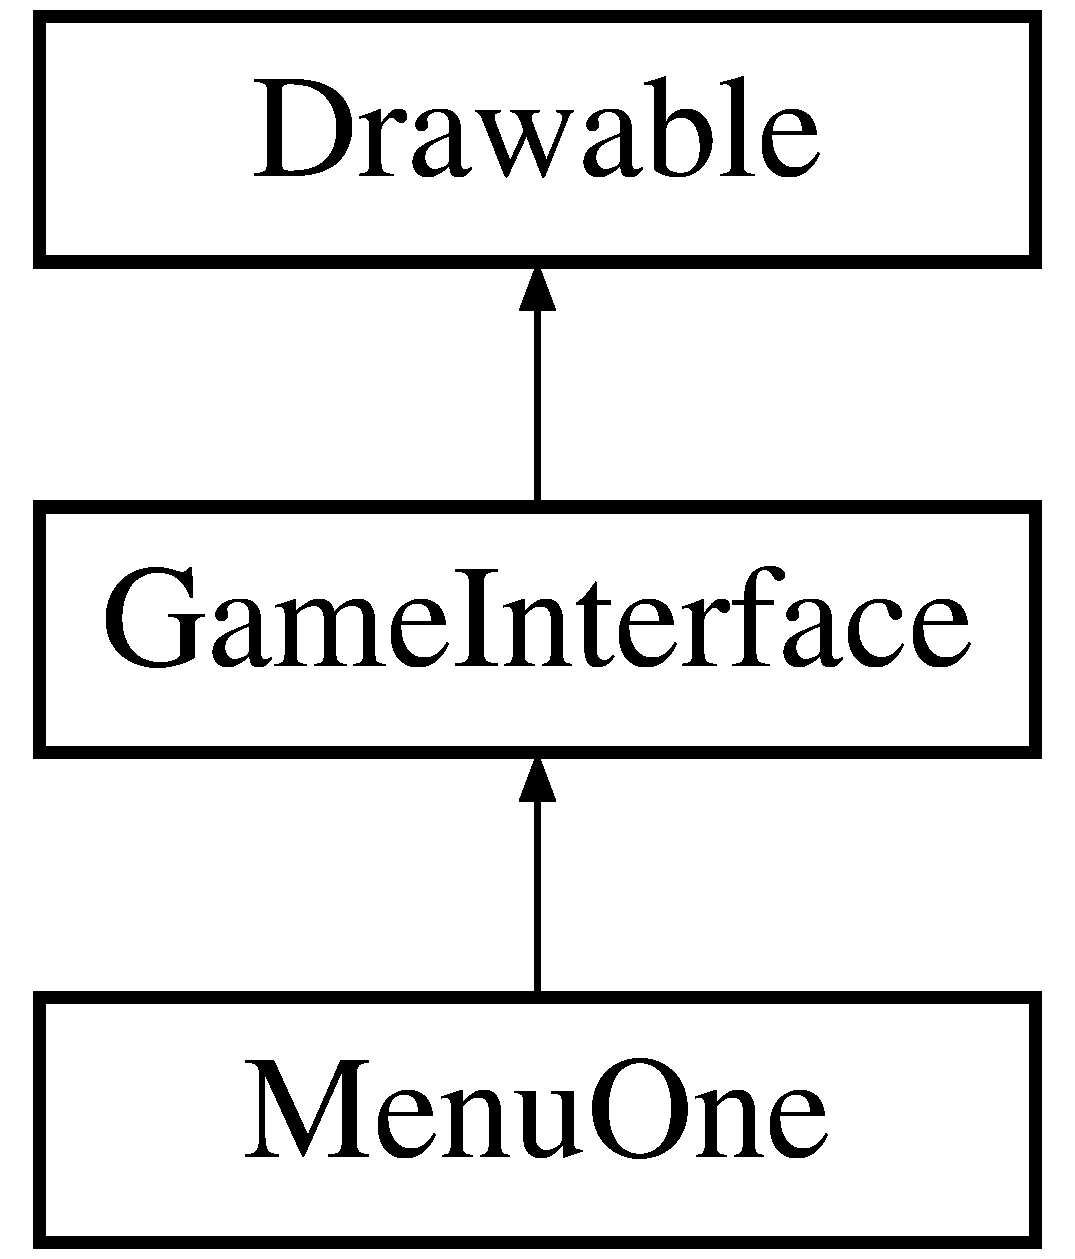
\includegraphics[height=3.000000cm]{class_menu_one}
\end{center}
\end{figure}
\subsection*{Public Member Functions}
\begin{DoxyCompactItemize}
\item 
\mbox{\Hypertarget{class_menu_one_af646b18d41ccf6412d40c4534c87859b}\label{class_menu_one_af646b18d41ccf6412d40c4534c87859b}} 
\mbox{\hyperlink{class_menu_one_af646b18d41ccf6412d40c4534c87859b}{Menu\+One}} ()
\begin{DoxyCompactList}\small\item\em Constructor. \end{DoxyCompactList}\item 
\mbox{\Hypertarget{class_menu_one_a42980aef723c12ee5fcb3a7b2be9490e}\label{class_menu_one_a42980aef723c12ee5fcb3a7b2be9490e}} 
\mbox{\hyperlink{class_menu_one_a42980aef723c12ee5fcb3a7b2be9490e}{$\sim$\+Menu\+One}} ()
\begin{DoxyCompactList}\small\item\em Deconstructor. \end{DoxyCompactList}\item 
\mbox{\Hypertarget{class_menu_one_ac0d1bdcb57588c6efd661979afd384e1}\label{class_menu_one_ac0d1bdcb57588c6efd661979afd384e1}} 
void \mbox{\hyperlink{class_menu_one_ac0d1bdcb57588c6efd661979afd384e1}{update\+Game}} (float p\+\_\+time) override
\begin{DoxyCompactList}\small\item\em update the menu \end{DoxyCompactList}\item 
void \mbox{\hyperlink{class_menu_one_a861529b6fcc30daebc753186714e3cc9}{draw}} (sf\+::\+Render\+Target \&target, sf\+::\+Render\+States states) const override
\begin{DoxyCompactList}\small\item\em draw the menu \end{DoxyCompactList}\item 
void \mbox{\hyperlink{class_menu_one_aee28812124909d8734eeeaecfde35f0f}{handle\+Input}} (int p\+\_\+\+Input\+Event) override
\begin{DoxyCompactList}\small\item\em Handles menu input. \end{DoxyCompactList}\item 
virtual End\+State \mbox{\hyperlink{class_menu_one_aa1d50806994903b77d44d241d7755404}{is\+Over}} () override
\begin{DoxyCompactList}\small\item\em What is the end stae. \end{DoxyCompactList}\item 
\mbox{\Hypertarget{class_menu_one_ae4b7ffe12a5e54975c2cf7c75982c47b}\label{class_menu_one_ae4b7ffe12a5e54975c2cf7c75982c47b}} 
virtual void \mbox{\hyperlink{class_menu_one_ae4b7ffe12a5e54975c2cf7c75982c47b}{load\+Level}} () override
\begin{DoxyCompactList}\small\item\em Load the level. \end{DoxyCompactList}\item 
\mbox{\Hypertarget{class_menu_one_a62021e82a91bcfefe2508c1abc89af39}\label{class_menu_one_a62021e82a91bcfefe2508c1abc89af39}} 
int \mbox{\hyperlink{class_menu_one_a62021e82a91bcfefe2508c1abc89af39}{get\+Level}} ()
\begin{DoxyCompactList}\small\item\em Get the level. \end{DoxyCompactList}\end{DoxyCompactItemize}
\subsection*{Private Attributes}
\begin{DoxyCompactItemize}
\item 
\mbox{\Hypertarget{class_menu_one_adc87ccaf60520d5eff34b4132e09a9e4}\label{class_menu_one_adc87ccaf60520d5eff34b4132e09a9e4}} 
\mbox{\hyperlink{class_file_reader_game_assests}{File\+Reader\+Game\+Assests}} $\ast$ \mbox{\hyperlink{class_menu_one_adc87ccaf60520d5eff34b4132e09a9e4}{m\+\_\+reader}}
\begin{DoxyCompactList}\small\item\em Game Assests reader. \end{DoxyCompactList}\item 
\mbox{\Hypertarget{class_menu_one_a7d04616d482ed54b3f84b6f9e3b4de09}\label{class_menu_one_a7d04616d482ed54b3f84b6f9e3b4de09}} 
sf\+::\+Sprite \mbox{\hyperlink{class_menu_one_a7d04616d482ed54b3f84b6f9e3b4de09}{m\+\_\+s\+Background}}
\begin{DoxyCompactList}\small\item\em Backround. \end{DoxyCompactList}\item 
\mbox{\Hypertarget{class_menu_one_a53ba11130fd8062dfbf49bbea7726266}\label{class_menu_one_a53ba11130fd8062dfbf49bbea7726266}} 
sf\+::\+Texture \mbox{\hyperlink{class_menu_one_a53ba11130fd8062dfbf49bbea7726266}{m\+\_\+t\+Background}}
\begin{DoxyCompactList}\small\item\em Texture of background. \end{DoxyCompactList}\item 
\mbox{\Hypertarget{class_menu_one_a4d39bd33df8d3fcbf177ff096f6ff453}\label{class_menu_one_a4d39bd33df8d3fcbf177ff096f6ff453}} 
std\+::vector$<$ sf\+::\+Sprite $\ast$ $>$ \mbox{\hyperlink{class_menu_one_a4d39bd33df8d3fcbf177ff096f6ff453}{m\+\_\+s\+Buttons}}
\begin{DoxyCompactList}\small\item\em Buttons on the menu. \end{DoxyCompactList}\item 
\mbox{\Hypertarget{class_menu_one_af8eb4784fa6e62496705c89e9aab7d86}\label{class_menu_one_af8eb4784fa6e62496705c89e9aab7d86}} 
sf\+::\+Texture \mbox{\hyperlink{class_menu_one_af8eb4784fa6e62496705c89e9aab7d86}{m\+\_\+t\+Buttons}}
\begin{DoxyCompactList}\small\item\em Texture of those buttons. \end{DoxyCompactList}\item 
\mbox{\Hypertarget{class_menu_one_a1e7bb22ae51a05f0927fd01e05ea3116}\label{class_menu_one_a1e7bb22ae51a05f0927fd01e05ea3116}} 
sf\+::\+Sprite \mbox{\hyperlink{class_menu_one_a1e7bb22ae51a05f0927fd01e05ea3116}{m\+\_\+s\+Selector}}
\begin{DoxyCompactList}\small\item\em The selector changing what the button looks like. \end{DoxyCompactList}\item 
\mbox{\Hypertarget{class_menu_one_a8bd621656e2106144772e92ce2e1d42c}\label{class_menu_one_a8bd621656e2106144772e92ce2e1d42c}} 
sf\+::\+Texture \mbox{\hyperlink{class_menu_one_a8bd621656e2106144772e92ce2e1d42c}{m\+\_\+t\+Selector}}
\begin{DoxyCompactList}\small\item\em Texture of the changer. \end{DoxyCompactList}\item 
\mbox{\Hypertarget{class_menu_one_a785b997d5cc3bb1515ba61f45971624a}\label{class_menu_one_a785b997d5cc3bb1515ba61f45971624a}} 
sf\+::\+Font \mbox{\hyperlink{class_menu_one_a785b997d5cc3bb1515ba61f45971624a}{m\+\_\+font}}
\begin{DoxyCompactList}\small\item\em Menu Font. \end{DoxyCompactList}\item 
\mbox{\Hypertarget{class_menu_one_a36b54bfaec07fa54a752649fdd29954f}\label{class_menu_one_a36b54bfaec07fa54a752649fdd29954f}} 
sf\+::\+Text \mbox{\hyperlink{class_menu_one_a36b54bfaec07fa54a752649fdd29954f}{m\+\_\+menu\+Text}}
\begin{DoxyCompactList}\small\item\em Text on the menu. \end{DoxyCompactList}\item 
\mbox{\Hypertarget{class_menu_one_aa80508cb857fab740bef53b81affd3e0}\label{class_menu_one_aa80508cb857fab740bef53b81affd3e0}} 
std\+::vector$<$ sf\+::\+Text $\ast$ $>$ \mbox{\hyperlink{class_menu_one_aa80508cb857fab740bef53b81affd3e0}{m\+\_\+button\+Text}}
\begin{DoxyCompactList}\small\item\em Text in the button. \end{DoxyCompactList}\item 
\mbox{\Hypertarget{class_menu_one_a56f390ef6e56c20246fa6b5cca02e181}\label{class_menu_one_a56f390ef6e56c20246fa6b5cca02e181}} 
\mbox{\hyperlink{class_texture_handler}{Texture\+Handler}} $\ast$ \mbox{\hyperlink{class_menu_one_a56f390ef6e56c20246fa6b5cca02e181}{m\+\_\+textures}}
\begin{DoxyCompactList}\small\item\em Texture Handler. \end{DoxyCompactList}\item 
\mbox{\Hypertarget{class_menu_one_ab8b2c807616861d67f442b7757012479}\label{class_menu_one_ab8b2c807616861d67f442b7757012479}} 
int \mbox{\hyperlink{class_menu_one_ab8b2c807616861d67f442b7757012479}{m\+\_\+current\+Level}}
\begin{DoxyCompactList}\small\item\em Stores the current level. \end{DoxyCompactList}\item 
\mbox{\Hypertarget{class_menu_one_a7b8b398cbbcd5702c7fa27a5546d0ca1}\label{class_menu_one_a7b8b398cbbcd5702c7fa27a5546d0ca1}} 
End\+State \mbox{\hyperlink{class_menu_one_a7b8b398cbbcd5702c7fa27a5546d0ca1}{m\+\_\+over}}
\begin{DoxyCompactList}\small\item\em End state is stored here. \end{DoxyCompactList}\end{DoxyCompactItemize}
\subsection*{Additional Inherited Members}


\subsection{Detailed Description}
This class is used for the starting menu\textquotesingle{}s it allows the user what level they want to play 

\subsection{Member Function Documentation}
\mbox{\Hypertarget{class_menu_one_a861529b6fcc30daebc753186714e3cc9}\label{class_menu_one_a861529b6fcc30daebc753186714e3cc9}} 
\index{Menu\+One@{Menu\+One}!draw@{draw}}
\index{draw@{draw}!Menu\+One@{Menu\+One}}
\subsubsection{\texorpdfstring{draw()}{draw()}}
{\footnotesize\ttfamily void Menu\+One\+::draw (\begin{DoxyParamCaption}\item[{sf\+::\+Render\+Target \&}]{target,  }\item[{sf\+::\+Render\+States}]{states }\end{DoxyParamCaption}) const\hspace{0.3cm}{\ttfamily [override]}, {\ttfamily [virtual]}}



draw the menu 


\begin{DoxyParams}{Parameters}
{\em p\+\_\+time} & contains information on the time \\
\hline
\end{DoxyParams}


Implements \mbox{\hyperlink{class_game_interface_ab33712e6b22b934982896ea0cab1699a}{Game\+Interface}}.

\mbox{\Hypertarget{class_menu_one_aee28812124909d8734eeeaecfde35f0f}\label{class_menu_one_aee28812124909d8734eeeaecfde35f0f}} 
\index{Menu\+One@{Menu\+One}!handle\+Input@{handle\+Input}}
\index{handle\+Input@{handle\+Input}!Menu\+One@{Menu\+One}}
\subsubsection{\texorpdfstring{handle\+Input()}{handleInput()}}
{\footnotesize\ttfamily void Menu\+One\+::handle\+Input (\begin{DoxyParamCaption}\item[{int}]{p\+\_\+\+Input\+Event }\end{DoxyParamCaption})\hspace{0.3cm}{\ttfamily [override]}, {\ttfamily [virtual]}}



Handles menu input. 


\begin{DoxyParams}{Parameters}
{\em target} & draw this \\
\hline
{\em states} & paramater needed for the draw method \\
\hline
\end{DoxyParams}


Implements \mbox{\hyperlink{class_game_interface_a48b4f6059c14c79359d30b77016a28f0}{Game\+Interface}}.

\mbox{\Hypertarget{class_menu_one_aa1d50806994903b77d44d241d7755404}\label{class_menu_one_aa1d50806994903b77d44d241d7755404}} 
\index{Menu\+One@{Menu\+One}!is\+Over@{is\+Over}}
\index{is\+Over@{is\+Over}!Menu\+One@{Menu\+One}}
\subsubsection{\texorpdfstring{is\+Over()}{isOver()}}
{\footnotesize\ttfamily virtual End\+State Menu\+One\+::is\+Over (\begin{DoxyParamCaption}{ }\end{DoxyParamCaption})\hspace{0.3cm}{\ttfamily [override]}, {\ttfamily [virtual]}}



What is the end stae. 


\begin{DoxyParams}{Parameters}
{\em p\+\_\+\+Input\+Event} & information needed to know what key is pressed \\
\hline
\end{DoxyParams}


Implements \mbox{\hyperlink{class_game_interface_a5bad60f237214cb1ec013e221ed16f45}{Game\+Interface}}.



The documentation for this class was generated from the following file\+:\begin{DoxyCompactItemize}
\item 
C\+:/\+Users/\+The Stormtrooper/\+Source/\+Repos/\+Final\+Year\+Project9/\+Vampires\+Vs\+Knights/include/Menu\+One.\+h\end{DoxyCompactItemize}

\hypertarget{class_node_interface}{}\section{Node\+Interface Class Reference}
\label{class_node_interface}\index{Node\+Interface@{Node\+Interface}}


{\ttfamily \#include $<$Node\+Interface.\+h$>$}

Inheritance diagram for Node\+Interface\+:\begin{figure}[H]
\begin{center}
\leavevmode
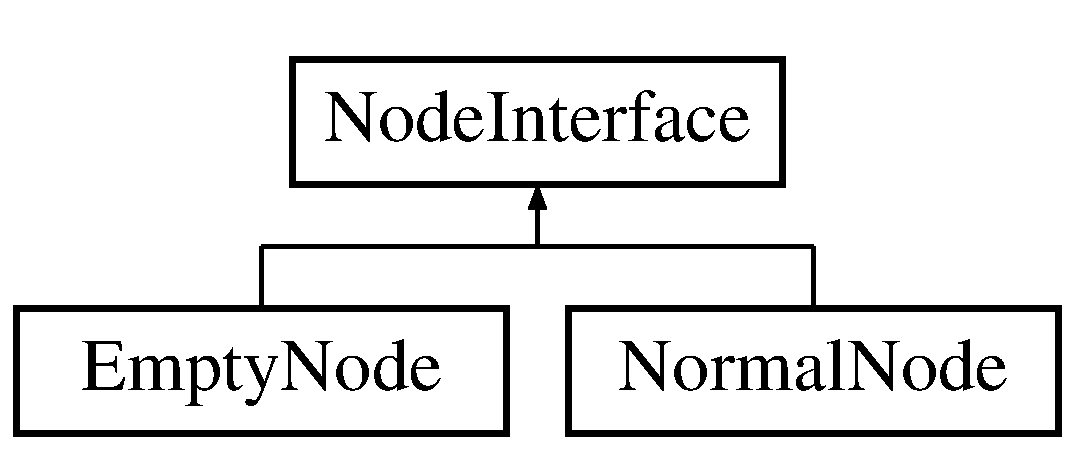
\includegraphics[height=2.000000cm]{class_node_interface}
\end{center}
\end{figure}
\subsection*{Public Member Functions}
\begin{DoxyCompactItemize}
\item 
\mbox{\Hypertarget{class_node_interface_a3d79c567537e9ffa7d2fc821495879fb}\label{class_node_interface_a3d79c567537e9ffa7d2fc821495879fb}} 
virtual sf\+::\+Sprite $\ast$ \mbox{\hyperlink{class_node_interface_a3d79c567537e9ffa7d2fc821495879fb}{get\+Sprite}} ()=0
\begin{DoxyCompactList}\small\item\em Gets the sprite of the node so its drawn. \end{DoxyCompactList}\item 
\mbox{\Hypertarget{class_node_interface_aba153b8ff03f15ce596887357a11aed8}\label{class_node_interface_aba153b8ff03f15ce596887357a11aed8}} 
virtual void \mbox{\hyperlink{class_node_interface_aba153b8ff03f15ce596887357a11aed8}{construct\+Node}} (int p\+\_\+row, int p\+\_\+col, sf\+::\+Texture p\+\_\+T)=0
\begin{DoxyCompactList}\small\item\em Constructs Node. \end{DoxyCompactList}\item 
virtual void \mbox{\hyperlink{class_node_interface_a9aeb69f061905e96ef6b1983c7a88fe3}{update\+Node}} (float p\+\_\+time)=0
\begin{DoxyCompactList}\small\item\em Updates the game. \end{DoxyCompactList}\item 
virtual std\+::string \mbox{\hyperlink{class_node_interface_a944dbfa74de55bdef1d583f318888aeb}{check\+Node\+Type}} ()=0
\begin{DoxyCompactList}\small\item\em Checks the type of the node. \end{DoxyCompactList}\item 
\mbox{\Hypertarget{class_node_interface_acc8dffd1dde9232e7541fff5b54783f0}\label{class_node_interface_acc8dffd1dde9232e7541fff5b54783f0}} 
virtual float {\bfseries getG} ()
\item 
\mbox{\Hypertarget{class_node_interface_a934ef1f220c6f61fa86200bd19586224}\label{class_node_interface_a934ef1f220c6f61fa86200bd19586224}} 
virtual float \mbox{\hyperlink{class_node_interface_a934ef1f220c6f61fa86200bd19586224}{getH}} ()
\begin{DoxyCompactList}\small\item\em Get the G value. \end{DoxyCompactList}\item 
\mbox{\Hypertarget{class_node_interface_abb64234aaa72e26967985af6a3eef54d}\label{class_node_interface_abb64234aaa72e26967985af6a3eef54d}} 
virtual float \mbox{\hyperlink{class_node_interface_abb64234aaa72e26967985af6a3eef54d}{getF}} ()
\begin{DoxyCompactList}\small\item\em Get the H value. \end{DoxyCompactList}\item 
\mbox{\Hypertarget{class_node_interface_a3071ba4b47011558bf75ba0de9a1b8bb}\label{class_node_interface_a3071ba4b47011558bf75ba0de9a1b8bb}} 
virtual float \mbox{\hyperlink{class_node_interface_a3071ba4b47011558bf75ba0de9a1b8bb}{get\+Terrain\+Cost}} ()
\begin{DoxyCompactList}\small\item\em Get the F value. \end{DoxyCompactList}\item 
\mbox{\Hypertarget{class_node_interface_a667925c62ad01dea0f5943cea165c533}\label{class_node_interface_a667925c62ad01dea0f5943cea165c533}} 
virtual sf\+::\+Vector2i \mbox{\hyperlink{class_node_interface_a667925c62ad01dea0f5943cea165c533}{get\+ID}} ()
\begin{DoxyCompactList}\small\item\em Get Cost. \end{DoxyCompactList}\item 
\mbox{\Hypertarget{class_node_interface_a1bb8d872c0b8f0794bf621be24ea0ca3}\label{class_node_interface_a1bb8d872c0b8f0794bf621be24ea0ca3}} 
virtual void \mbox{\hyperlink{class_node_interface_a1bb8d872c0b8f0794bf621be24ea0ca3}{setG}} (float p\+\_\+g)
\begin{DoxyCompactList}\small\item\em Get id. \end{DoxyCompactList}\item 
virtual void \mbox{\hyperlink{class_node_interface_a8750e3c16815db5f6bae6de6b3335a8f}{setF}} (float p\+\_\+f)
\begin{DoxyCompactList}\small\item\em Set G. \end{DoxyCompactList}\item 
virtual void \mbox{\hyperlink{class_node_interface_a4159fd7efddfb97216b7b6b4916bf003}{setH}} (float p\+\_\+H)
\begin{DoxyCompactList}\small\item\em Set F. \end{DoxyCompactList}\item 
virtual void \mbox{\hyperlink{class_node_interface_a759b060003767c5319c1c568705696e0}{set\+Diagonal}} (bool p\+\_\+b)
\begin{DoxyCompactList}\small\item\em Set H. \end{DoxyCompactList}\item 
virtual \mbox{\hyperlink{class_node_interface}{Node\+Interface}} $\ast$ \mbox{\hyperlink{class_node_interface_ade5a090eeac6a245475f49589c79be8a}{get\+Perant}} ()
\begin{DoxyCompactList}\small\item\em Set Diagonal method. \end{DoxyCompactList}\item 
\mbox{\Hypertarget{class_node_interface_a6b1ea79473c66ffc69454d798943d4a0}\label{class_node_interface_a6b1ea79473c66ffc69454d798943d4a0}} 
virtual void \mbox{\hyperlink{class_node_interface_a6b1ea79473c66ffc69454d798943d4a0}{set\+Perant}} (\mbox{\hyperlink{class_node_interface}{Node\+Interface}} $\ast$p\+\_\+\+NI)
\begin{DoxyCompactList}\small\item\em Get the perant of the node. \end{DoxyCompactList}\item 
virtual bool \mbox{\hyperlink{class_node_interface_a4baa534fe0139637524fcd05cf9f5fe6}{is\+Diagonal}} ()
\begin{DoxyCompactList}\small\item\em Set the perant. \end{DoxyCompactList}\end{DoxyCompactItemize}
\subsection*{Protected Attributes}
\begin{DoxyCompactItemize}
\item 
sf\+::\+Sprite $\ast$ \mbox{\hyperlink{class_node_interface_a11c603f391c23f2ea6c7ff228f8f40e6}{m\+\_\+sprite}}
\begin{DoxyCompactList}\small\item\em Is it Diagonal. \end{DoxyCompactList}\item 
\mbox{\Hypertarget{class_node_interface_ac3ba2fd8d5ec51b3432a6092d059131a}\label{class_node_interface_ac3ba2fd8d5ec51b3432a6092d059131a}} 
sf\+::\+Texture \mbox{\hyperlink{class_node_interface_ac3ba2fd8d5ec51b3432a6092d059131a}{m\+\_\+texture}}
\begin{DoxyCompactList}\small\item\em Contains texture. \end{DoxyCompactList}\item 
\mbox{\Hypertarget{class_node_interface_a221bbac677de84cd72b03ec14322f6d4}\label{class_node_interface_a221bbac677de84cd72b03ec14322f6d4}} 
\mbox{\hyperlink{class_node_interface}{Node\+Interface}} $\ast$ \mbox{\hyperlink{class_node_interface_a221bbac677de84cd72b03ec14322f6d4}{m\+\_\+perant}}
\begin{DoxyCompactList}\small\item\em Stores pointer to the perant. \end{DoxyCompactList}\item 
\mbox{\Hypertarget{class_node_interface_a90b046dd5869a936ecfd91e381693d50}\label{class_node_interface_a90b046dd5869a936ecfd91e381693d50}} 
sf\+::\+Vector2i \mbox{\hyperlink{class_node_interface_a90b046dd5869a936ecfd91e381693d50}{m\+\_\+id}}
\begin{DoxyCompactList}\small\item\em Stores id. \end{DoxyCompactList}\item 
\mbox{\Hypertarget{class_node_interface_a4d839e467a94e8f68d0a92dd63d51c58}\label{class_node_interface_a4d839e467a94e8f68d0a92dd63d51c58}} 
float \mbox{\hyperlink{class_node_interface_a4d839e467a94e8f68d0a92dd63d51c58}{m\+\_\+movement\+Cost}}
\begin{DoxyCompactList}\small\item\em stores movment cost \end{DoxyCompactList}\item 
\mbox{\Hypertarget{class_node_interface_a93fbc84071fcaefe031ae65927701814}\label{class_node_interface_a93fbc84071fcaefe031ae65927701814}} 
float \mbox{\hyperlink{class_node_interface_a93fbc84071fcaefe031ae65927701814}{m\+\_\+f\+Value}}
\begin{DoxyCompactList}\small\item\em Store F. \end{DoxyCompactList}\item 
\mbox{\Hypertarget{class_node_interface_af3c69e17a7eb84a082001443d7670d3c}\label{class_node_interface_af3c69e17a7eb84a082001443d7670d3c}} 
float \mbox{\hyperlink{class_node_interface_af3c69e17a7eb84a082001443d7670d3c}{m\+\_\+g\+Value}}
\begin{DoxyCompactList}\small\item\em Store G. \end{DoxyCompactList}\item 
\mbox{\Hypertarget{class_node_interface_af6dd7f4959cfb1a8402a7202060eacc2}\label{class_node_interface_af6dd7f4959cfb1a8402a7202060eacc2}} 
float \mbox{\hyperlink{class_node_interface_af6dd7f4959cfb1a8402a7202060eacc2}{m\+\_\+h\+Value}}
\begin{DoxyCompactList}\small\item\em Set H. \end{DoxyCompactList}\item 
\mbox{\Hypertarget{class_node_interface_aa0366b52d789726dfef6a806f1081dd9}\label{class_node_interface_aa0366b52d789726dfef6a806f1081dd9}} 
bool \mbox{\hyperlink{class_node_interface_aa0366b52d789726dfef6a806f1081dd9}{m\+\_\+is\+Diagonal}}
\begin{DoxyCompactList}\small\item\em Stores bool. \end{DoxyCompactList}\end{DoxyCompactItemize}


\subsection{Detailed Description}
States what each node must have, if i wanted a new type of Node i could inherit from this and not worry about copying this code 

\subsection{Member Function Documentation}
\mbox{\Hypertarget{class_node_interface_a944dbfa74de55bdef1d583f318888aeb}\label{class_node_interface_a944dbfa74de55bdef1d583f318888aeb}} 
\index{Node\+Interface@{Node\+Interface}!check\+Node\+Type@{check\+Node\+Type}}
\index{check\+Node\+Type@{check\+Node\+Type}!Node\+Interface@{Node\+Interface}}
\subsubsection{\texorpdfstring{check\+Node\+Type()}{checkNodeType()}}
{\footnotesize\ttfamily virtual std\+::string Node\+Interface\+::check\+Node\+Type (\begin{DoxyParamCaption}{ }\end{DoxyParamCaption})\hspace{0.3cm}{\ttfamily [pure virtual]}}



Checks the type of the node. 


\begin{DoxyParams}{Parameters}
{\em p\+\_\+time} & contains information on the time \\
\hline
\end{DoxyParams}


Implemented in \mbox{\hyperlink{class_empty_node_a2281f852354a5b95ba06f4e2a7e8de34}{Empty\+Node}}, and \mbox{\hyperlink{class_normal_node_aa11cbf32f7395ce3fd01113942c6351f}{Normal\+Node}}.

\mbox{\Hypertarget{class_node_interface_ade5a090eeac6a245475f49589c79be8a}\label{class_node_interface_ade5a090eeac6a245475f49589c79be8a}} 
\index{Node\+Interface@{Node\+Interface}!get\+Perant@{get\+Perant}}
\index{get\+Perant@{get\+Perant}!Node\+Interface@{Node\+Interface}}
\subsubsection{\texorpdfstring{get\+Perant()}{getPerant()}}
{\footnotesize\ttfamily virtual \mbox{\hyperlink{class_node_interface}{Node\+Interface}}$\ast$ Node\+Interface\+::get\+Perant (\begin{DoxyParamCaption}{ }\end{DoxyParamCaption})\hspace{0.3cm}{\ttfamily [inline]}, {\ttfamily [virtual]}}



Set Diagonal method. 


\begin{DoxyParams}{Parameters}
{\em p\+\_\+b} & information of the m\+\_\+is\+Diaognal \\
\hline
\end{DoxyParams}
\mbox{\Hypertarget{class_node_interface_a4baa534fe0139637524fcd05cf9f5fe6}\label{class_node_interface_a4baa534fe0139637524fcd05cf9f5fe6}} 
\index{Node\+Interface@{Node\+Interface}!is\+Diagonal@{is\+Diagonal}}
\index{is\+Diagonal@{is\+Diagonal}!Node\+Interface@{Node\+Interface}}
\subsubsection{\texorpdfstring{is\+Diagonal()}{isDiagonal()}}
{\footnotesize\ttfamily virtual bool Node\+Interface\+::is\+Diagonal (\begin{DoxyParamCaption}{ }\end{DoxyParamCaption})\hspace{0.3cm}{\ttfamily [inline]}, {\ttfamily [virtual]}}



Set the perant. 


\begin{DoxyParams}{Parameters}
{\em p\+\_\+\+NI} & the node that will be set as the perant \\
\hline
\end{DoxyParams}
\mbox{\Hypertarget{class_node_interface_a759b060003767c5319c1c568705696e0}\label{class_node_interface_a759b060003767c5319c1c568705696e0}} 
\index{Node\+Interface@{Node\+Interface}!set\+Diagonal@{set\+Diagonal}}
\index{set\+Diagonal@{set\+Diagonal}!Node\+Interface@{Node\+Interface}}
\subsubsection{\texorpdfstring{set\+Diagonal()}{setDiagonal()}}
{\footnotesize\ttfamily virtual void Node\+Interface\+::set\+Diagonal (\begin{DoxyParamCaption}\item[{bool}]{p\+\_\+b }\end{DoxyParamCaption})\hspace{0.3cm}{\ttfamily [inline]}, {\ttfamily [virtual]}}



Set H. 


\begin{DoxyParams}{Parameters}
{\em p\+\_\+h} & information on the H value \\
\hline
\end{DoxyParams}
\mbox{\Hypertarget{class_node_interface_a8750e3c16815db5f6bae6de6b3335a8f}\label{class_node_interface_a8750e3c16815db5f6bae6de6b3335a8f}} 
\index{Node\+Interface@{Node\+Interface}!setF@{setF}}
\index{setF@{setF}!Node\+Interface@{Node\+Interface}}
\subsubsection{\texorpdfstring{set\+F()}{setF()}}
{\footnotesize\ttfamily virtual void Node\+Interface\+::setF (\begin{DoxyParamCaption}\item[{float}]{p\+\_\+f }\end{DoxyParamCaption})\hspace{0.3cm}{\ttfamily [inline]}, {\ttfamily [virtual]}}



Set G. 


\begin{DoxyParams}{Parameters}
{\em p\+\_\+g} & information on the G value \\
\hline
\end{DoxyParams}
\mbox{\Hypertarget{class_node_interface_a4159fd7efddfb97216b7b6b4916bf003}\label{class_node_interface_a4159fd7efddfb97216b7b6b4916bf003}} 
\index{Node\+Interface@{Node\+Interface}!setH@{setH}}
\index{setH@{setH}!Node\+Interface@{Node\+Interface}}
\subsubsection{\texorpdfstring{set\+H()}{setH()}}
{\footnotesize\ttfamily virtual void Node\+Interface\+::setH (\begin{DoxyParamCaption}\item[{float}]{p\+\_\+H }\end{DoxyParamCaption})\hspace{0.3cm}{\ttfamily [inline]}, {\ttfamily [virtual]}}



Set F. 


\begin{DoxyParams}{Parameters}
{\em p\+\_\+f} & information on the F value \\
\hline
\end{DoxyParams}
\mbox{\Hypertarget{class_node_interface_a9aeb69f061905e96ef6b1983c7a88fe3}\label{class_node_interface_a9aeb69f061905e96ef6b1983c7a88fe3}} 
\index{Node\+Interface@{Node\+Interface}!update\+Node@{update\+Node}}
\index{update\+Node@{update\+Node}!Node\+Interface@{Node\+Interface}}
\subsubsection{\texorpdfstring{update\+Node()}{updateNode()}}
{\footnotesize\ttfamily virtual void Node\+Interface\+::update\+Node (\begin{DoxyParamCaption}\item[{float}]{p\+\_\+time }\end{DoxyParamCaption})\hspace{0.3cm}{\ttfamily [pure virtual]}}



Updates the game. 


\begin{DoxyParams}{Parameters}
{\em p\+\_\+row} & the row the node is on \\
\hline
{\em p\+\_\+col} & the column the row is on \\
\hline
{\em p\+\_\+T} & the texture of the node \\
\hline
\end{DoxyParams}


Implemented in \mbox{\hyperlink{class_empty_node_ae11626adf3ad771cfcc68599c67ff354}{Empty\+Node}}, and \mbox{\hyperlink{class_normal_node_a4a846f6117353fe7483e1348a4da6e1f}{Normal\+Node}}.



\subsection{Member Data Documentation}
\mbox{\Hypertarget{class_node_interface_a11c603f391c23f2ea6c7ff228f8f40e6}\label{class_node_interface_a11c603f391c23f2ea6c7ff228f8f40e6}} 
\index{Node\+Interface@{Node\+Interface}!m\+\_\+sprite@{m\+\_\+sprite}}
\index{m\+\_\+sprite@{m\+\_\+sprite}!Node\+Interface@{Node\+Interface}}
\subsubsection{\texorpdfstring{m\+\_\+sprite}{m\_sprite}}
{\footnotesize\ttfamily sf\+::\+Sprite$\ast$ Node\+Interface\+::m\+\_\+sprite\hspace{0.3cm}{\ttfamily [protected]}}



Is it Diagonal. 

Contains node sprite 

The documentation for this class was generated from the following file\+:\begin{DoxyCompactItemize}
\item 
C\+:/\+Users/\+The Stormtrooper/\+Source/\+Repos/\+Final\+Year\+Project9/\+Vampires\+Vs\+Knights/include/Node\+Interface.\+h\end{DoxyCompactItemize}

\hypertarget{class_normal_node}{}\section{Normal\+Node Class Reference}
\label{class_normal_node}\index{Normal\+Node@{Normal\+Node}}


{\ttfamily \#include $<$Normal\+Node.\+h$>$}

Inheritance diagram for Normal\+Node\+:\begin{figure}[H]
\begin{center}
\leavevmode
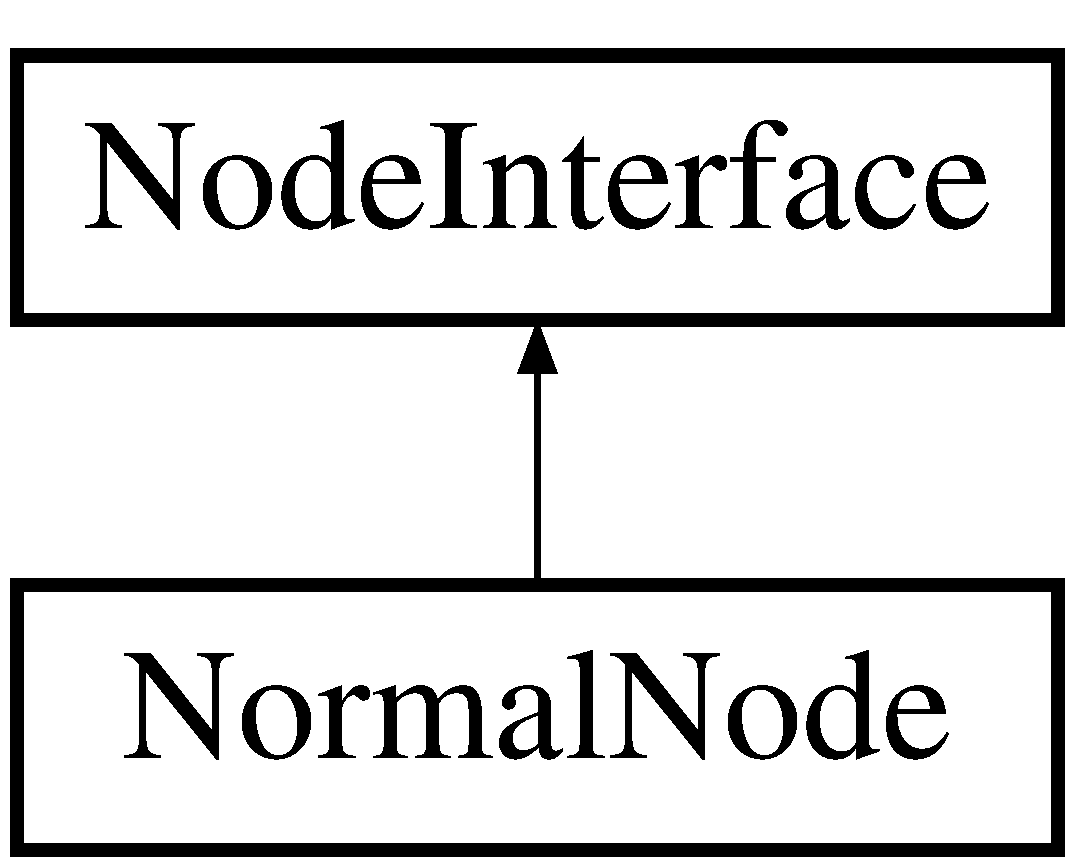
\includegraphics[height=2.000000cm]{class_normal_node}
\end{center}
\end{figure}
\subsection*{Public Member Functions}
\begin{DoxyCompactItemize}
\item 
\mbox{\Hypertarget{class_normal_node_a98d7475e5063b8ead0e0a15f7c0cdeef}\label{class_normal_node_a98d7475e5063b8ead0e0a15f7c0cdeef}} 
\mbox{\hyperlink{class_normal_node_a98d7475e5063b8ead0e0a15f7c0cdeef}{Normal\+Node}} (int p\+\_\+cost)
\begin{DoxyCompactList}\small\item\em Construct Node. \end{DoxyCompactList}\item 
\mbox{\hyperlink{class_normal_node_a0a046b69544c8cc7e352dca9b5837b76}{$\sim$\+Normal\+Node}} ()
\begin{DoxyCompactList}\small\item\em Deconstructor. \end{DoxyCompactList}\item 
\mbox{\Hypertarget{class_normal_node_a4a846f6117353fe7483e1348a4da6e1f}\label{class_normal_node_a4a846f6117353fe7483e1348a4da6e1f}} 
void \mbox{\hyperlink{class_normal_node_a4a846f6117353fe7483e1348a4da6e1f}{update\+Node}} (float p\+\_\+time) override
\begin{DoxyCompactList}\small\item\em Update method. \end{DoxyCompactList}\item 
sf\+::\+Sprite $\ast$ \mbox{\hyperlink{class_normal_node_aa5b5cb046635230adf5356e8bd0a61c2}{get\+Sprite}} () override
\begin{DoxyCompactList}\small\item\em Get sprite of node. \end{DoxyCompactList}\item 
\mbox{\Hypertarget{class_normal_node_a7b75fb9660c92491bb797b030538c8f5}\label{class_normal_node_a7b75fb9660c92491bb797b030538c8f5}} 
void \mbox{\hyperlink{class_normal_node_a7b75fb9660c92491bb797b030538c8f5}{construct\+Node}} (int p\+\_\+x, int p\+\_\+y, sf\+::\+Texture p\+\_\+T) override
\begin{DoxyCompactList}\small\item\em Construct node. \end{DoxyCompactList}\item 
\mbox{\Hypertarget{class_normal_node_aa11cbf32f7395ce3fd01113942c6351f}\label{class_normal_node_aa11cbf32f7395ce3fd01113942c6351f}} 
std\+::string \mbox{\hyperlink{class_normal_node_aa11cbf32f7395ce3fd01113942c6351f}{check\+Node\+Type}} () override
\begin{DoxyCompactList}\small\item\em get node type \end{DoxyCompactList}\end{DoxyCompactItemize}
\subsection*{Additional Inherited Members}


\subsection{Detailed Description}
A node that the user can move too 

\subsection{Constructor \& Destructor Documentation}
\mbox{\Hypertarget{class_normal_node_a0a046b69544c8cc7e352dca9b5837b76}\label{class_normal_node_a0a046b69544c8cc7e352dca9b5837b76}} 
\index{Normal\+Node@{Normal\+Node}!````~Normal\+Node@{$\sim$\+Normal\+Node}}
\index{````~Normal\+Node@{$\sim$\+Normal\+Node}!Normal\+Node@{Normal\+Node}}
\subsubsection{\texorpdfstring{$\sim$\+Normal\+Node()}{~NormalNode()}}
{\footnotesize\ttfamily Normal\+Node\+::$\sim$\+Normal\+Node (\begin{DoxyParamCaption}{ }\end{DoxyParamCaption})}



Deconstructor. 


\begin{DoxyParams}{Parameters}
{\em p\+\_\+cost} & the cost of the current node \\
\hline
\end{DoxyParams}


\subsection{Member Function Documentation}
\mbox{\Hypertarget{class_normal_node_aa5b5cb046635230adf5356e8bd0a61c2}\label{class_normal_node_aa5b5cb046635230adf5356e8bd0a61c2}} 
\index{Normal\+Node@{Normal\+Node}!get\+Sprite@{get\+Sprite}}
\index{get\+Sprite@{get\+Sprite}!Normal\+Node@{Normal\+Node}}
\subsubsection{\texorpdfstring{get\+Sprite()}{getSprite()}}
{\footnotesize\ttfamily sf\+::\+Sprite$\ast$ Normal\+Node\+::get\+Sprite (\begin{DoxyParamCaption}{ }\end{DoxyParamCaption})\hspace{0.3cm}{\ttfamily [override]}, {\ttfamily [virtual]}}



Get sprite of node. 


\begin{DoxyParams}{Parameters}
{\em p\+\_\+time} & contains information on the time \\
\hline
\end{DoxyParams}


Implements \mbox{\hyperlink{class_node_interface_a3d79c567537e9ffa7d2fc821495879fb}{Node\+Interface}}.



The documentation for this class was generated from the following file\+:\begin{DoxyCompactItemize}
\item 
C\+:/\+Users/\+The Stormtrooper/\+Source/\+Repos/\+Final\+Year\+Project9/\+Vampires\+Vs\+Knights/include/Normal\+Node.\+h\end{DoxyCompactItemize}

\hypertarget{class_scene}{}\section{Scene Class Reference}
\label{class_scene}\index{Scene@{Scene}}


{\ttfamily \#include $<$Scene.\+h$>$}

Inheritance diagram for Scene\+:\begin{figure}[H]
\begin{center}
\leavevmode
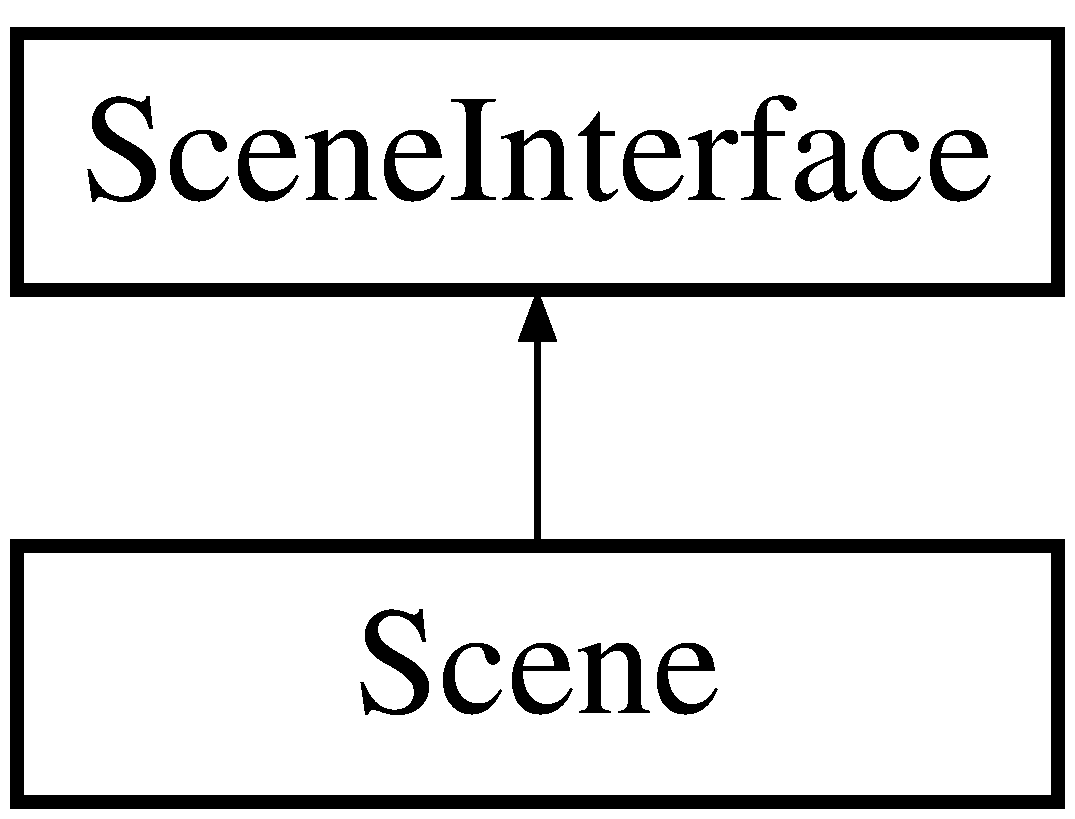
\includegraphics[height=2.000000cm]{class_scene}
\end{center}
\end{figure}
\subsection*{Public Member Functions}
\begin{DoxyCompactItemize}
\item 
\mbox{\Hypertarget{class_scene_ac0b5325e1196ae9fb1a4d1d6adde0795}\label{class_scene_ac0b5325e1196ae9fb1a4d1d6adde0795}} 
void \mbox{\hyperlink{class_scene_ac0b5325e1196ae9fb1a4d1d6adde0795}{update\+Scene}} (float p\+\_\+time) override
\begin{DoxyCompactList}\small\item\em Update scene. \end{DoxyCompactList}\item 
bool \mbox{\hyperlink{class_scene_a27a8b36b21dd9475d47c13db8cfdae64}{load\+Level}} (std\+::string p\+\_\+level) override
\begin{DoxyCompactList}\small\item\em Load level. \end{DoxyCompactList}\item 
std\+::vector$<$ sf\+::\+Sprite $\ast$ $>$ \mbox{\hyperlink{class_scene_a595b66ffbd3efe4a0dd40f704a84c378}{get\+Sprite\+Vector}} () override
\begin{DoxyCompactList}\small\item\em Gets a vector of sprites to draw. \end{DoxyCompactList}\item 
\mbox{\Hypertarget{class_scene_a3a3d817613f8d775fd6fb244c54ec5b1}\label{class_scene_a3a3d817613f8d775fd6fb244c54ec5b1}} 
End\+State \mbox{\hyperlink{class_scene_a3a3d817613f8d775fd6fb244c54ec5b1}{get\+End\+State}} ()
\begin{DoxyCompactList}\small\item\em Gets the scenes end state. \end{DoxyCompactList}\item 
\mbox{\Hypertarget{class_scene_a7c64740eba60afdacf9622122b8a4348}\label{class_scene_a7c64740eba60afdacf9622122b8a4348}} 
int \mbox{\hyperlink{class_scene_a7c64740eba60afdacf9622122b8a4348}{get\+Round}} ()
\begin{DoxyCompactList}\small\item\em What round is it. \end{DoxyCompactList}\item 
\mbox{\Hypertarget{class_scene_a507df51d6597c3e84590c579a26d0856}\label{class_scene_a507df51d6597c3e84590c579a26d0856}} 
void \mbox{\hyperlink{class_scene_a507df51d6597c3e84590c579a26d0856}{check\+Stats}} ()
\begin{DoxyCompactList}\small\item\em Display the units stats. \end{DoxyCompactList}\item 
\mbox{\Hypertarget{class_scene_af2908989883758468fc2add26b3637e6}\label{class_scene_af2908989883758468fc2add26b3637e6}} 
sf\+::\+Sprite \mbox{\hyperlink{class_scene_af2908989883758468fc2add26b3637e6}{get\+Selector}} ()
\begin{DoxyCompactList}\small\item\em Gets the selector to draw. \end{DoxyCompactList}\item 
\mbox{\Hypertarget{class_scene_ac8eec69b021a9cd85f39aaaeb9de8785}\label{class_scene_ac8eec69b021a9cd85f39aaaeb9de8785}} 
void \mbox{\hyperlink{class_scene_ac8eec69b021a9cd85f39aaaeb9de8785}{increment\+Selector}} (sf\+::\+Vector2i p\+\_\+new\+Pos)
\begin{DoxyCompactList}\small\item\em Moves the selector. \end{DoxyCompactList}\item 
void \mbox{\hyperlink{class_scene_a2b3d2bde3505a1626ad5c8435025e9fc}{decrease\+Selector}} (sf\+::\+Vector2i p\+\_\+new\+Pos)
\begin{DoxyCompactList}\small\item\em Moves the selector down. \end{DoxyCompactList}\item 
void \mbox{\hyperlink{class_scene_a33e61bb927aa8a3e1070a907ffff24a5}{Players\+Move}} ()
\begin{DoxyCompactList}\small\item\em When the player hits enter key there move begins. \end{DoxyCompactList}\item 
\mbox{\Hypertarget{class_scene_a3ebc1a157e63088eb47ff6cea6dd6d56}\label{class_scene_a3ebc1a157e63088eb47ff6cea6dd6d56}} 
\mbox{\hyperlink{class_h_u_d}{H\+UD}} $\ast$ \mbox{\hyperlink{class_scene_a3ebc1a157e63088eb47ff6cea6dd6d56}{get\+H\+UD}} () override
\begin{DoxyCompactList}\small\item\em Gets the \mbox{\hyperlink{class_h_u_d}{H\+UD}}. \end{DoxyCompactList}\item 
\mbox{\Hypertarget{class_scene_a8a67c7ff953a4808b45981f8a40bafa3}\label{class_scene_a8a67c7ff953a4808b45981f8a40bafa3}} 
\mbox{\hyperlink{class_scene_a8a67c7ff953a4808b45981f8a40bafa3}{Scene}} (std\+::string p\+\_\+characters, std\+::string p\+\_\+nodes)
\begin{DoxyCompactList}\small\item\em Constructor. \end{DoxyCompactList}\item 
\mbox{\hyperlink{class_scene_a3b8cec2e32546713915f8c6303c951f1}{$\sim$\+Scene}} ()
\begin{DoxyCompactList}\small\item\em Deconstructor. \end{DoxyCompactList}\end{DoxyCompactItemize}
\subsection*{Private Attributes}
\begin{DoxyCompactItemize}
\item 
\mbox{\Hypertarget{class_scene_a8d7c43876336f52c76a288532e681c7c}\label{class_scene_a8d7c43876336f52c76a288532e681c7c}} 
bool \mbox{\hyperlink{class_scene_a8d7c43876336f52c76a288532e681c7c}{playerkilled}}
\begin{DoxyCompactList}\small\item\em Was a unit killed. \end{DoxyCompactList}\item 
\mbox{\Hypertarget{class_scene_a5d79aa70e9ac8b5851ad8c28d5629c35}\label{class_scene_a5d79aa70e9ac8b5851ad8c28d5629c35}} 
bool \mbox{\hyperlink{class_scene_a5d79aa70e9ac8b5851ad8c28d5629c35}{m\+\_\+reached\+Goal}}
\begin{DoxyCompactList}\small\item\em Did the unit reach the goal. \end{DoxyCompactList}\item 
\mbox{\Hypertarget{class_scene_a70a2c4620c467044155309b945fe4c33}\label{class_scene_a70a2c4620c467044155309b945fe4c33}} 
\mbox{\hyperlink{class_texture_handler}{Texture\+Handler}} $\ast$ \mbox{\hyperlink{class_scene_a70a2c4620c467044155309b945fe4c33}{m\+\_\+texture\+Handler}}
\begin{DoxyCompactList}\small\item\em Texture Handler. \end{DoxyCompactList}\item 
\mbox{\Hypertarget{class_scene_a3736d22281ac82fd3a16f434487442d3}\label{class_scene_a3736d22281ac82fd3a16f434487442d3}} 
\mbox{\hyperlink{class_file_reader}{File\+Reader}} $\ast$ \mbox{\hyperlink{class_scene_a3736d22281ac82fd3a16f434487442d3}{m\+\_\+file\+Reader}}
\begin{DoxyCompactList}\small\item\em File reader. \end{DoxyCompactList}\item 
\mbox{\Hypertarget{class_scene_a2191f78a6e675382488cdaca6e371c32}\label{class_scene_a2191f78a6e675382488cdaca6e371c32}} 
\mbox{\hyperlink{class_sprite_interface}{Sprite\+Interface}} $\ast$ \mbox{\hyperlink{class_scene_a2191f78a6e675382488cdaca6e371c32}{Target}}
\begin{DoxyCompactList}\small\item\em pointer to a target \end{DoxyCompactList}\item 
\mbox{\Hypertarget{class_scene_ab736eefd11ca6f4b90c0240895c316c4}\label{class_scene_ab736eefd11ca6f4b90c0240895c316c4}} 
Game\+State \mbox{\hyperlink{class_scene_ab736eefd11ca6f4b90c0240895c316c4}{m\+\_\+game\+State}}
\begin{DoxyCompactList}\small\item\em Stores the games current state. \end{DoxyCompactList}\item 
\mbox{\Hypertarget{class_scene_abf242918885f639abdb059385a35dfda}\label{class_scene_abf242918885f639abdb059385a35dfda}} 
End\+State \mbox{\hyperlink{class_scene_abf242918885f639abdb059385a35dfda}{m\+\_\+game\+Over\+State}}
\begin{DoxyCompactList}\small\item\em Stores the end state. \end{DoxyCompactList}\item 
\mbox{\Hypertarget{class_scene_aa2a82603f5db50e33fae8f444c6986ac}\label{class_scene_aa2a82603f5db50e33fae8f444c6986ac}} 
sf\+::\+Sprite \mbox{\hyperlink{class_scene_aa2a82603f5db50e33fae8f444c6986ac}{m\+\_\+selector}}
\begin{DoxyCompactList}\small\item\em Sprite of the selector. \end{DoxyCompactList}\item 
\mbox{\Hypertarget{class_scene_a1bfd679d50e896a6e56e73690001eb8b}\label{class_scene_a1bfd679d50e896a6e56e73690001eb8b}} 
sf\+::\+Texture \mbox{\hyperlink{class_scene_a1bfd679d50e896a6e56e73690001eb8b}{m\+\_\+selector\+Texture}}
\begin{DoxyCompactList}\small\item\em Texture of the selector. \end{DoxyCompactList}\item 
\mbox{\Hypertarget{class_scene_a30daf51f6f59d17c526be427856457ce}\label{class_scene_a30daf51f6f59d17c526be427856457ce}} 
sf\+::\+Vector2i \mbox{\hyperlink{class_scene_a30daf51f6f59d17c526be427856457ce}{m\+\_\+selector\+Pos}}
\begin{DoxyCompactList}\small\item\em Position of the selector. \end{DoxyCompactList}\item 
\mbox{\Hypertarget{class_scene_ae5339ca6ff15be177b1ed83f5a894801}\label{class_scene_ae5339ca6ff15be177b1ed83f5a894801}} 
std\+::vector$<$ \mbox{\hyperlink{class_sprite_interface}{Sprite\+Interface}} $\ast$ $>$ \mbox{\hyperlink{class_scene_ae5339ca6ff15be177b1ed83f5a894801}{m\+\_\+vector\+Sprites}}
\begin{DoxyCompactList}\small\item\em A vector of all the sprites. \end{DoxyCompactList}\item 
\mbox{\Hypertarget{class_scene_a4f25002a15f8f1549f8337bc84ff83e4}\label{class_scene_a4f25002a15f8f1549f8337bc84ff83e4}} 
\mbox{\hyperlink{class_sprite_interface}{Sprite\+Interface}} $\ast$ \mbox{\hyperlink{class_scene_a4f25002a15f8f1549f8337bc84ff83e4}{m\+\_\+player\+Temp}}
\begin{DoxyCompactList}\small\item\em stores a temp of the player \end{DoxyCompactList}\item 
\mbox{\Hypertarget{class_scene_abb000b09241752a5acc17bdcd3936c6e}\label{class_scene_abb000b09241752a5acc17bdcd3936c6e}} 
int \mbox{\hyperlink{class_scene_abb000b09241752a5acc17bdcd3936c6e}{current\+Player}}
\begin{DoxyCompactList}\small\item\em What is the current player. \end{DoxyCompactList}\item 
\mbox{\Hypertarget{class_scene_a012fe2d4370deb5bdac43bd5e607ca42}\label{class_scene_a012fe2d4370deb5bdac43bd5e607ca42}} 
int \mbox{\hyperlink{class_scene_a012fe2d4370deb5bdac43bd5e607ca42}{current\+Target}}
\begin{DoxyCompactList}\small\item\em What is the current target. \end{DoxyCompactList}\item 
\mbox{\Hypertarget{class_scene_a3c8813c62033911d9a602a49a8beca76}\label{class_scene_a3c8813c62033911d9a602a49a8beca76}} 
int \mbox{\hyperlink{class_scene_a3c8813c62033911d9a602a49a8beca76}{startof\+Knights}}
\begin{DoxyCompactList}\small\item\em what is the start of the knights in the vector \end{DoxyCompactList}\item 
\mbox{\Hypertarget{class_scene_a903aebbd9a63f70dbb9df52a253e83ce}\label{class_scene_a903aebbd9a63f70dbb9df52a253e83ce}} 
int \mbox{\hyperlink{class_scene_a903aebbd9a63f70dbb9df52a253e83ce}{startof\+Vampires}}
\begin{DoxyCompactList}\small\item\em Was a unit killed. \end{DoxyCompactList}\item 
\mbox{\Hypertarget{class_scene_a4a072bf6c3a790daef87ff8268e4556d}\label{class_scene_a4a072bf6c3a790daef87ff8268e4556d}} 
int \mbox{\hyperlink{class_scene_a4a072bf6c3a790daef87ff8268e4556d}{total\+Characters}}
\begin{DoxyCompactList}\small\item\em How many characters are ther. \end{DoxyCompactList}\item 
\mbox{\Hypertarget{class_scene_abbb010c89e64b117c17ed75fbfd13e49}\label{class_scene_abbb010c89e64b117c17ed75fbfd13e49}} 
bool \mbox{\hyperlink{class_scene_abbb010c89e64b117c17ed75fbfd13e49}{newcurrent\+Player}}
\begin{DoxyCompactList}\small\item\em is there a new current player \end{DoxyCompactList}\item 
\mbox{\Hypertarget{class_scene_ade40d20e64f9d4ccc1448936b47b9c00}\label{class_scene_ade40d20e64f9d4ccc1448936b47b9c00}} 
std\+::vector$<$ sf\+::\+Sprite $\ast$ $>$ \mbox{\hyperlink{class_scene_ade40d20e64f9d4ccc1448936b47b9c00}{m\+\_\+vector\+Temp}}
\begin{DoxyCompactList}\small\item\em A temp vector containing sprites. \end{DoxyCompactList}\item 
\mbox{\Hypertarget{class_scene_a91f8a53d7d0e9f6087baa3fa30c432e4}\label{class_scene_a91f8a53d7d0e9f6087baa3fa30c432e4}} 
std\+::list$<$ \mbox{\hyperlink{class_node_interface}{Node\+Interface}} $\ast$ $>$ \mbox{\hyperlink{class_scene_a91f8a53d7d0e9f6087baa3fa30c432e4}{m\+\_\+path\+List}}
\begin{DoxyCompactList}\small\item\em path the unit must take \end{DoxyCompactList}\item 
\mbox{\Hypertarget{class_scene_ad0e56315eddcb1259330fcd33340cdf6}\label{class_scene_ad0e56315eddcb1259330fcd33340cdf6}} 
\mbox{\hyperlink{class_node_interface}{Node\+Interface}} $\ast$ \mbox{\hyperlink{class_scene_ad0e56315eddcb1259330fcd33340cdf6}{m\+\_\+prevoius\+Node}}
\begin{DoxyCompactList}\small\item\em Pointer to the prevoius node. \end{DoxyCompactList}\item 
\mbox{\Hypertarget{class_scene_af60873fd6cdd2e5c28ab765866d048f5}\label{class_scene_af60873fd6cdd2e5c28ab765866d048f5}} 
\mbox{\hyperlink{class_node_interface}{Node\+Interface}} $\ast$ \mbox{\hyperlink{class_scene_af60873fd6cdd2e5c28ab765866d048f5}{temp}}
\begin{DoxyCompactList}\small\item\em Holds on to a node. \end{DoxyCompactList}\item 
\mbox{\Hypertarget{class_scene_a4d3a38106693ded1bbdc4bc850711bc0}\label{class_scene_a4d3a38106693ded1bbdc4bc850711bc0}} 
\mbox{\hyperlink{class_graph}{Graph}} $\ast$ \mbox{\hyperlink{class_scene_a4d3a38106693ded1bbdc4bc850711bc0}{m\+\_\+\+Graph}}
\begin{DoxyCompactList}\small\item\em Game object \mbox{\hyperlink{class_graph}{Graph}} used to create the grid. \end{DoxyCompactList}\item 
\mbox{\Hypertarget{class_scene_afb32c22792c8aeb990d043e3abd79c7e}\label{class_scene_afb32c22792c8aeb990d043e3abd79c7e}} 
\mbox{\hyperlink{class_h_u_d}{H\+UD}} $\ast$ \mbox{\hyperlink{class_scene_afb32c22792c8aeb990d043e3abd79c7e}{m\+\_\+game\+Hud}}
\begin{DoxyCompactList}\small\item\em Game object used to display some text to the screen. \end{DoxyCompactList}\item 
\mbox{\Hypertarget{class_scene_afbc60d92daf6a7ce27403484313b1dcb}\label{class_scene_afbc60d92daf6a7ce27403484313b1dcb}} 
int \mbox{\hyperlink{class_scene_afbc60d92daf6a7ce27403484313b1dcb}{m\+\_\+round}}
\begin{DoxyCompactList}\small\item\em Stores the current round. \end{DoxyCompactList}\item 
\mbox{\Hypertarget{class_scene_a6aaf00569c8fb13c0f970effb31ad340}\label{class_scene_a6aaf00569c8fb13c0f970effb31ad340}} 
int \mbox{\hyperlink{class_scene_a6aaf00569c8fb13c0f970effb31ad340}{current\+Enemy}}
\begin{DoxyCompactList}\small\item\em What is the current enemy. \end{DoxyCompactList}\item 
\mbox{\Hypertarget{class_scene_a082957d9d74447aa8acbb7192074510e}\label{class_scene_a082957d9d74447aa8acbb7192074510e}} 
float \mbox{\hyperlink{class_scene_a082957d9d74447aa8acbb7192074510e}{m\+\_\+time}}
\begin{DoxyCompactList}\small\item\em Stores the time. \end{DoxyCompactList}\item 
\mbox{\Hypertarget{class_scene_a39f11954b4d7250aeedc2a60e78fbb18}\label{class_scene_a39f11954b4d7250aeedc2a60e78fbb18}} 
float \mbox{\hyperlink{class_scene_a39f11954b4d7250aeedc2a60e78fbb18}{moving\+Counter}}
\begin{DoxyCompactList}\small\item\em counter used to slow characters down \end{DoxyCompactList}\end{DoxyCompactItemize}
\subsection*{Additional Inherited Members}


\subsection{Detailed Description}
This handles a lot of the game logic, each new scene can have diffrent nodes, characters etc 

\subsection{Constructor \& Destructor Documentation}
\mbox{\Hypertarget{class_scene_a3b8cec2e32546713915f8c6303c951f1}\label{class_scene_a3b8cec2e32546713915f8c6303c951f1}} 
\index{Scene@{Scene}!````~Scene@{$\sim$\+Scene}}
\index{````~Scene@{$\sim$\+Scene}!Scene@{Scene}}
\subsubsection{\texorpdfstring{$\sim$\+Scene()}{~Scene()}}
{\footnotesize\ttfamily Scene\+::$\sim$\+Scene (\begin{DoxyParamCaption}{ }\end{DoxyParamCaption})}



Deconstructor. 


\begin{DoxyParams}{Parameters}
{\em p\+\_\+characaters} & contains information the game scharacaters \\
\hline
{\em p\+\_\+nodes} & contains information the game nodes \\
\hline
\end{DoxyParams}


\subsection{Member Function Documentation}
\mbox{\Hypertarget{class_scene_a2b3d2bde3505a1626ad5c8435025e9fc}\label{class_scene_a2b3d2bde3505a1626ad5c8435025e9fc}} 
\index{Scene@{Scene}!decrease\+Selector@{decrease\+Selector}}
\index{decrease\+Selector@{decrease\+Selector}!Scene@{Scene}}
\subsubsection{\texorpdfstring{decrease\+Selector()}{decreaseSelector()}}
{\footnotesize\ttfamily void Scene\+::decrease\+Selector (\begin{DoxyParamCaption}\item[{sf\+::\+Vector2i}]{p\+\_\+new\+Pos }\end{DoxyParamCaption})}



Moves the selector down. 


\begin{DoxyParams}{Parameters}
{\em p\+\_\+new\+Pos} & used to move the selector \\
\hline
\end{DoxyParams}
\mbox{\Hypertarget{class_scene_a595b66ffbd3efe4a0dd40f704a84c378}\label{class_scene_a595b66ffbd3efe4a0dd40f704a84c378}} 
\index{Scene@{Scene}!get\+Sprite\+Vector@{get\+Sprite\+Vector}}
\index{get\+Sprite\+Vector@{get\+Sprite\+Vector}!Scene@{Scene}}
\subsubsection{\texorpdfstring{get\+Sprite\+Vector()}{getSpriteVector()}}
{\footnotesize\ttfamily std\+::vector$<$sf\+::\+Sprite$\ast$$>$ Scene\+::get\+Sprite\+Vector (\begin{DoxyParamCaption}{ }\end{DoxyParamCaption})\hspace{0.3cm}{\ttfamily [override]}, {\ttfamily [virtual]}}



Gets a vector of sprites to draw. 


\begin{DoxyParams}{Parameters}
{\em p\+\_\+level} & passes in level information \\
\hline
\end{DoxyParams}


Implements \mbox{\hyperlink{class_scene_interface_af4cdfa0df6cbbba34d66870ea83b2a0a}{Scene\+Interface}}.

\mbox{\Hypertarget{class_scene_a27a8b36b21dd9475d47c13db8cfdae64}\label{class_scene_a27a8b36b21dd9475d47c13db8cfdae64}} 
\index{Scene@{Scene}!load\+Level@{load\+Level}}
\index{load\+Level@{load\+Level}!Scene@{Scene}}
\subsubsection{\texorpdfstring{load\+Level()}{loadLevel()}}
{\footnotesize\ttfamily bool Scene\+::load\+Level (\begin{DoxyParamCaption}\item[{std\+::string}]{p\+\_\+level }\end{DoxyParamCaption})\hspace{0.3cm}{\ttfamily [override]}, {\ttfamily [virtual]}}



Load level. 


\begin{DoxyParams}{Parameters}
{\em p\+\_\+time} & contains information on the time \\
\hline
\end{DoxyParams}


Implements \mbox{\hyperlink{class_scene_interface_a54c0b8784bcb2278aeb9b6030df9a158}{Scene\+Interface}}.

\mbox{\Hypertarget{class_scene_a33e61bb927aa8a3e1070a907ffff24a5}\label{class_scene_a33e61bb927aa8a3e1070a907ffff24a5}} 
\index{Scene@{Scene}!Players\+Move@{Players\+Move}}
\index{Players\+Move@{Players\+Move}!Scene@{Scene}}
\subsubsection{\texorpdfstring{Players\+Move()}{PlayersMove()}}
{\footnotesize\ttfamily void Scene\+::\+Players\+Move (\begin{DoxyParamCaption}{ }\end{DoxyParamCaption})}



When the player hits enter key there move begins. 


\begin{DoxyParams}{Parameters}
{\em p\+\_\+new\+Pos} & used to move the selector \\
\hline
\end{DoxyParams}


The documentation for this class was generated from the following file\+:\begin{DoxyCompactItemize}
\item 
C\+:/\+Users/\+The Stormtrooper/\+Source/\+Repos/\+Final\+Year\+Project9/\+Vampires\+Vs\+Knights/include/Scene.\+h\end{DoxyCompactItemize}

\hypertarget{class_scene_interface}{}\section{Scene\+Interface Class Reference}
\label{class_scene_interface}\index{Scene\+Interface@{Scene\+Interface}}


{\ttfamily \#include $<$Scene\+Interface.\+h$>$}

Inheritance diagram for Scene\+Interface\+:\begin{figure}[H]
\begin{center}
\leavevmode
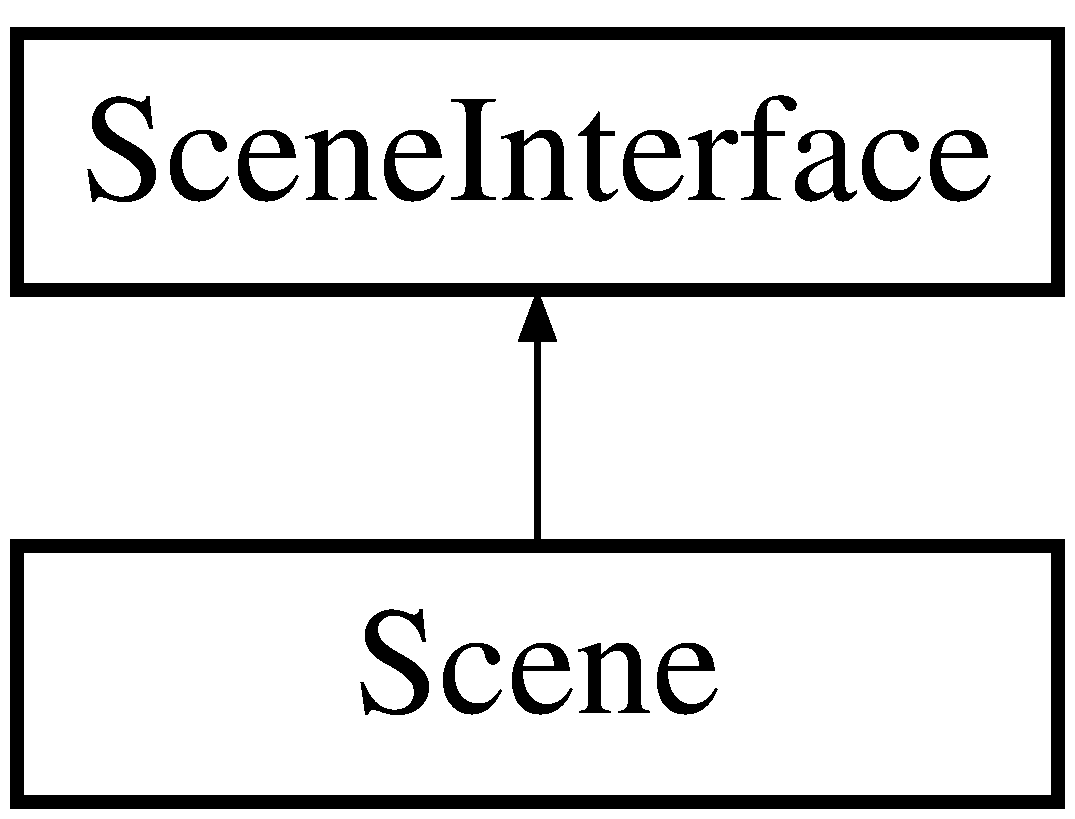
\includegraphics[height=2.000000cm]{class_scene_interface}
\end{center}
\end{figure}
\subsection*{Protected Member Functions}
\begin{DoxyCompactItemize}
\item 
\mbox{\Hypertarget{class_scene_interface_a3944b25997f846ce54128e10fccd69c5}\label{class_scene_interface_a3944b25997f846ce54128e10fccd69c5}} 
virtual void \mbox{\hyperlink{class_scene_interface_a3944b25997f846ce54128e10fccd69c5}{update\+Scene}} (float p\+\_\+time)=0
\begin{DoxyCompactList}\small\item\em Update method. \end{DoxyCompactList}\item 
virtual bool \mbox{\hyperlink{class_scene_interface_a54c0b8784bcb2278aeb9b6030df9a158}{load\+Level}} (std\+::string p\+\_\+level)=0
\begin{DoxyCompactList}\small\item\em load level \end{DoxyCompactList}\item 
virtual std\+::vector$<$ sf\+::\+Sprite $\ast$ $>$ \mbox{\hyperlink{class_scene_interface_af4cdfa0df6cbbba34d66870ea83b2a0a}{get\+Sprite\+Vector}} ()=0
\begin{DoxyCompactList}\small\item\em gets a list of sprites \end{DoxyCompactList}\item 
\mbox{\Hypertarget{class_scene_interface_a7c5194abd1f623d4e4da61779a164a12}\label{class_scene_interface_a7c5194abd1f623d4e4da61779a164a12}} 
virtual \mbox{\hyperlink{class_h_u_d}{H\+UD}} $\ast$ \mbox{\hyperlink{class_scene_interface_a7c5194abd1f623d4e4da61779a164a12}{get\+H\+UD}} ()=0
\begin{DoxyCompactList}\small\item\em Gets the \mbox{\hyperlink{class_h_u_d}{H\+UD}}. \end{DoxyCompactList}\end{DoxyCompactItemize}


\subsection{Detailed Description}
This states what every scene should have 

\subsection{Member Function Documentation}
\mbox{\Hypertarget{class_scene_interface_af4cdfa0df6cbbba34d66870ea83b2a0a}\label{class_scene_interface_af4cdfa0df6cbbba34d66870ea83b2a0a}} 
\index{Scene\+Interface@{Scene\+Interface}!get\+Sprite\+Vector@{get\+Sprite\+Vector}}
\index{get\+Sprite\+Vector@{get\+Sprite\+Vector}!Scene\+Interface@{Scene\+Interface}}
\subsubsection{\texorpdfstring{get\+Sprite\+Vector()}{getSpriteVector()}}
{\footnotesize\ttfamily virtual std\+::vector$<$sf\+::\+Sprite$\ast$$>$ Scene\+Interface\+::get\+Sprite\+Vector (\begin{DoxyParamCaption}{ }\end{DoxyParamCaption})\hspace{0.3cm}{\ttfamily [protected]}, {\ttfamily [pure virtual]}}



gets a list of sprites 


\begin{DoxyParams}{Parameters}
{\em p\+\_\+level} & contains information on the level \\
\hline
\end{DoxyParams}


Implemented in \mbox{\hyperlink{class_scene_a595b66ffbd3efe4a0dd40f704a84c378}{Scene}}.

\mbox{\Hypertarget{class_scene_interface_a54c0b8784bcb2278aeb9b6030df9a158}\label{class_scene_interface_a54c0b8784bcb2278aeb9b6030df9a158}} 
\index{Scene\+Interface@{Scene\+Interface}!load\+Level@{load\+Level}}
\index{load\+Level@{load\+Level}!Scene\+Interface@{Scene\+Interface}}
\subsubsection{\texorpdfstring{load\+Level()}{loadLevel()}}
{\footnotesize\ttfamily virtual bool Scene\+Interface\+::load\+Level (\begin{DoxyParamCaption}\item[{std\+::string}]{p\+\_\+level }\end{DoxyParamCaption})\hspace{0.3cm}{\ttfamily [protected]}, {\ttfamily [pure virtual]}}



load level 


\begin{DoxyParams}{Parameters}
{\em p\+\_\+time} & contains information on the time \\
\hline
\end{DoxyParams}


Implemented in \mbox{\hyperlink{class_scene_a27a8b36b21dd9475d47c13db8cfdae64}{Scene}}.



The documentation for this class was generated from the following file\+:\begin{DoxyCompactItemize}
\item 
C\+:/\+Users/\+The Stormtrooper/\+Source/\+Repos/\+Final\+Year\+Project9/\+Vampires\+Vs\+Knights/include/Scene\+Interface.\+h\end{DoxyCompactItemize}

\hypertarget{class_sprite_interface}{}\section{Sprite\+Interface Class Reference}
\label{class_sprite_interface}\index{Sprite\+Interface@{Sprite\+Interface}}


{\ttfamily \#include $<$Sprite\+Interface.\+h$>$}

Inheritance diagram for Sprite\+Interface\+:\begin{figure}[H]
\begin{center}
\leavevmode
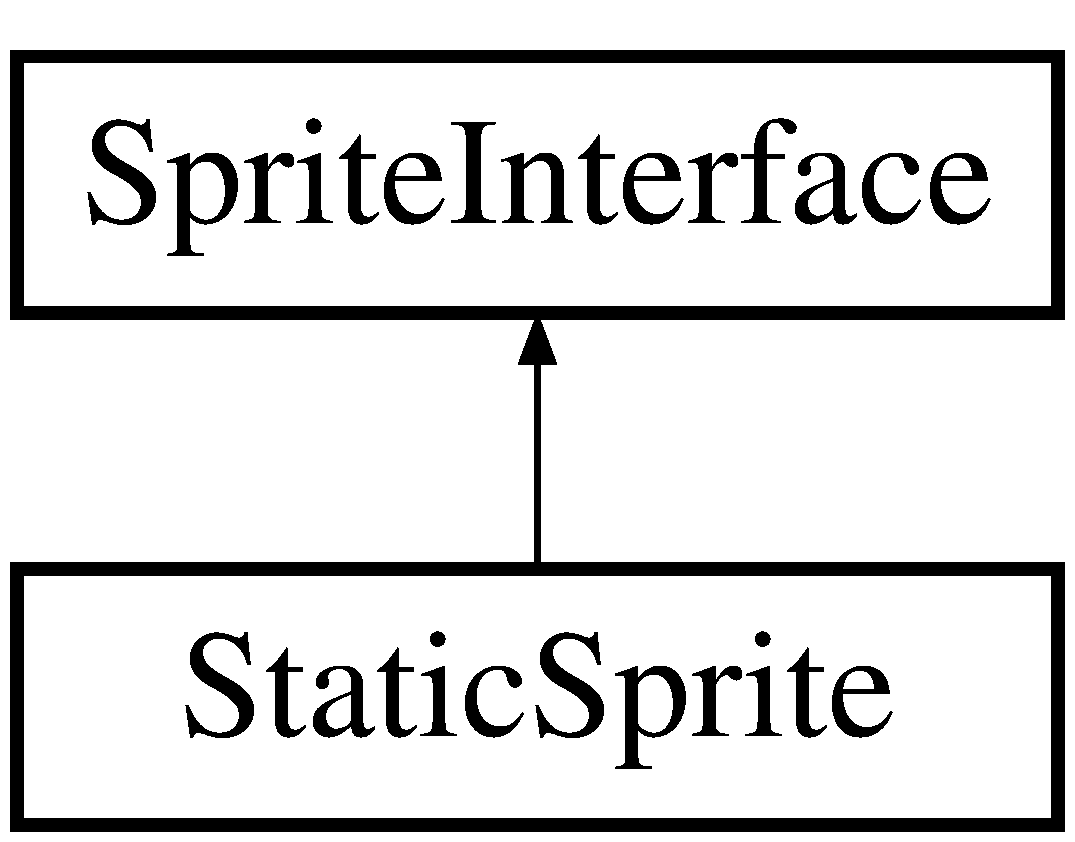
\includegraphics[height=2.000000cm]{class_sprite_interface}
\end{center}
\end{figure}
\subsection*{Public Member Functions}
\begin{DoxyCompactItemize}
\item 
\mbox{\Hypertarget{class_sprite_interface_ad3bcdb5a25c5fe0315c9938a7c8ed395}\label{class_sprite_interface_ad3bcdb5a25c5fe0315c9938a7c8ed395}} 
Sprite\+State \mbox{\hyperlink{class_sprite_interface_ad3bcdb5a25c5fe0315c9938a7c8ed395}{get\+State}} ()
\begin{DoxyCompactList}\small\item\em Gets the sprite state. \end{DoxyCompactList}\item 
\mbox{\Hypertarget{class_sprite_interface_a548fdaa1e0443386b42326e69702fc13}\label{class_sprite_interface_a548fdaa1e0443386b42326e69702fc13}} 
virtual sf\+::\+Sprite $\ast$ {\bfseries get\+Sprite} ()
\item 
\mbox{\Hypertarget{class_sprite_interface_aab826769df1222d5dd2ff426c8551bb2}\label{class_sprite_interface_aab826769df1222d5dd2ff426c8551bb2}} 
virtual void \mbox{\hyperlink{class_sprite_interface_aab826769df1222d5dd2ff426c8551bb2}{set\+Node}} (\mbox{\hyperlink{class_node_interface}{Node\+Interface}} $\ast$p\+\_\+\+NI)
\begin{DoxyCompactList}\small\item\em Gets the sprite. \end{DoxyCompactList}\item 
virtual \mbox{\hyperlink{class_node_interface}{Node\+Interface}} $\ast$ \mbox{\hyperlink{class_sprite_interface_a0cda548d74975cb3dd3f4d163a1763b6}{get\+Node}} ()
\begin{DoxyCompactList}\small\item\em Sets a node to each sprite. \end{DoxyCompactList}\item 
\mbox{\Hypertarget{class_sprite_interface_a69b0d3d856aa935d533e2d4ad323235a}\label{class_sprite_interface_a69b0d3d856aa935d533e2d4ad323235a}} 
virtual float \mbox{\hyperlink{class_sprite_interface_a69b0d3d856aa935d533e2d4ad323235a}{get\+Speed}} ()
\begin{DoxyCompactList}\small\item\em Gets the node within each sprite. \end{DoxyCompactList}\item 
\mbox{\Hypertarget{class_sprite_interface_a9acb8edb465672a3e55d0b972a20c768}\label{class_sprite_interface_a9acb8edb465672a3e55d0b972a20c768}} 
virtual float \mbox{\hyperlink{class_sprite_interface_a9acb8edb465672a3e55d0b972a20c768}{get\+Attack}} ()
\begin{DoxyCompactList}\small\item\em Sets characater speed. \end{DoxyCompactList}\item 
\mbox{\Hypertarget{class_sprite_interface_a4552ddf09fb794495ce4697c5af753b9}\label{class_sprite_interface_a4552ddf09fb794495ce4697c5af753b9}} 
virtual float \mbox{\hyperlink{class_sprite_interface_a4552ddf09fb794495ce4697c5af753b9}{get\+Health}} ()
\begin{DoxyCompactList}\small\item\em Get attack. \end{DoxyCompactList}\item 
virtual bool \mbox{\hyperlink{class_sprite_interface_a91a747b887e19cfc6e5256d4afc2f64c}{is\+Doing\+Damage}} ()=0
\begin{DoxyCompactList}\small\item\em Get Health. \end{DoxyCompactList}\item 
\mbox{\Hypertarget{class_sprite_interface_a98f300b8d8e40f3dcd18c853353a1ac9}\label{class_sprite_interface_a98f300b8d8e40f3dcd18c853353a1ac9}} 
virtual void \mbox{\hyperlink{class_sprite_interface_a98f300b8d8e40f3dcd18c853353a1ac9}{do\+Damage}} (bool p\+\_\+bool)=0
\begin{DoxyCompactList}\small\item\em Do the damage. \end{DoxyCompactList}\item 
virtual void \mbox{\hyperlink{class_sprite_interface_a56abad058843e3e4a7801f5b12cc6e18}{set\+Health}} (float p\+\_\+damage\+Taken)=0
\begin{DoxyCompactList}\small\item\em Takeaways from its current health. \end{DoxyCompactList}\item 
virtual void \mbox{\hyperlink{class_sprite_interface_a30511b7aaf2661d4f53db5b172dd365b}{set\+Sprite\+Pos}} (int p\+\_\+col, int p\+\_\+row)=0
\begin{DoxyCompactList}\small\item\em Sets its position. \end{DoxyCompactList}\item 
virtual void \mbox{\hyperlink{class_sprite_interface_ad5335c5370f97cd81a52769cb0a25559}{message}} (const std\+::string p\+\_\+message)=0
\begin{DoxyCompactList}\small\item\em Gives the sprite a message. \end{DoxyCompactList}\item 
virtual void \mbox{\hyperlink{class_sprite_interface_a3153bba12e2561f1719a75dbff0e6b4a}{update}} (float p\+\_\+time)=0
\begin{DoxyCompactList}\small\item\em Update method. \end{DoxyCompactList}\end{DoxyCompactItemize}
\subsection*{Protected Attributes}
\begin{DoxyCompactItemize}
\item 
sf\+::\+Sprite $\ast$ \mbox{\hyperlink{class_sprite_interface_ad39fe3c5309c30a22ddfce60fa9f7c09}{m\+\_\+sprite}}
\begin{DoxyCompactList}\small\item\em The sprite of the sprite. \end{DoxyCompactList}\item 
\mbox{\Hypertarget{class_sprite_interface_a6085987c42f63d186dfc69353dae76f1}\label{class_sprite_interface_a6085987c42f63d186dfc69353dae76f1}} 
sf\+::\+Texture \mbox{\hyperlink{class_sprite_interface_a6085987c42f63d186dfc69353dae76f1}{m\+\_\+texture}}
\begin{DoxyCompactList}\small\item\em Texture. \end{DoxyCompactList}\item 
\mbox{\Hypertarget{class_sprite_interface_a3535d0dbdd54673a67692aecac6c2052}\label{class_sprite_interface_a3535d0dbdd54673a67692aecac6c2052}} 
\mbox{\hyperlink{class_node_interface}{Node\+Interface}} $\ast$ \mbox{\hyperlink{class_sprite_interface_a3535d0dbdd54673a67692aecac6c2052}{m\+\_\+node}}
\begin{DoxyCompactList}\small\item\em Pointer to a node. \end{DoxyCompactList}\item 
\mbox{\Hypertarget{class_sprite_interface_ab06d7faea880bcf73267dffb3fcb855c}\label{class_sprite_interface_ab06d7faea880bcf73267dffb3fcb855c}} 
float \mbox{\hyperlink{class_sprite_interface_ab06d7faea880bcf73267dffb3fcb855c}{m\+\_\+speed}}
\begin{DoxyCompactList}\small\item\em Speed. \end{DoxyCompactList}\item 
\mbox{\Hypertarget{class_sprite_interface_a43bacc6a76b45b80ef61daafbcc879b5}\label{class_sprite_interface_a43bacc6a76b45b80ef61daafbcc879b5}} 
float \mbox{\hyperlink{class_sprite_interface_a43bacc6a76b45b80ef61daafbcc879b5}{m\+\_\+attack}}
\begin{DoxyCompactList}\small\item\em Attack. \end{DoxyCompactList}\item 
\mbox{\Hypertarget{class_sprite_interface_a8b0b188a190e0c1a7b30a7b0ca911b0f}\label{class_sprite_interface_a8b0b188a190e0c1a7b30a7b0ca911b0f}} 
float \mbox{\hyperlink{class_sprite_interface_a8b0b188a190e0c1a7b30a7b0ca911b0f}{m\+\_\+health}}
\begin{DoxyCompactList}\small\item\em H\+E\+A\+L\+TH. \end{DoxyCompactList}\item 
\mbox{\Hypertarget{class_sprite_interface_a161675cd2b32e41a30925da4617003b3}\label{class_sprite_interface_a161675cd2b32e41a30925da4617003b3}} 
bool \mbox{\hyperlink{class_sprite_interface_a161675cd2b32e41a30925da4617003b3}{m\+\_\+is\+Doing\+Damage}}
\begin{DoxyCompactList}\small\item\em Is it doing damage. \end{DoxyCompactList}\item 
\mbox{\Hypertarget{class_sprite_interface_a4a0986e0b5bd14defa82eb7d9fe1886e}\label{class_sprite_interface_a4a0986e0b5bd14defa82eb7d9fe1886e}} 
Sprite\+State \mbox{\hyperlink{class_sprite_interface_a4a0986e0b5bd14defa82eb7d9fe1886e}{m\+\_\+sprite\+State}}
\begin{DoxyCompactList}\small\item\em State of the sprite. \end{DoxyCompactList}\end{DoxyCompactItemize}


\subsection{Detailed Description}
States all the information a character should have 

\subsection{Member Function Documentation}
\mbox{\Hypertarget{class_sprite_interface_a0cda548d74975cb3dd3f4d163a1763b6}\label{class_sprite_interface_a0cda548d74975cb3dd3f4d163a1763b6}} 
\index{Sprite\+Interface@{Sprite\+Interface}!get\+Node@{get\+Node}}
\index{get\+Node@{get\+Node}!Sprite\+Interface@{Sprite\+Interface}}
\subsubsection{\texorpdfstring{get\+Node()}{getNode()}}
{\footnotesize\ttfamily virtual \mbox{\hyperlink{class_node_interface}{Node\+Interface}}$\ast$ Sprite\+Interface\+::get\+Node (\begin{DoxyParamCaption}{ }\end{DoxyParamCaption})\hspace{0.3cm}{\ttfamily [inline]}, {\ttfamily [virtual]}}



Sets a node to each sprite. 


\begin{DoxyParams}{Parameters}
{\em p\+\_\+\+NI} & this node will become m\+\_\+node \\
\hline
\end{DoxyParams}


Reimplemented in \mbox{\hyperlink{class_static_sprite_a672bb6e3425bbc15cd9034ab9e2802fd}{Static\+Sprite}}.

\mbox{\Hypertarget{class_sprite_interface_a91a747b887e19cfc6e5256d4afc2f64c}\label{class_sprite_interface_a91a747b887e19cfc6e5256d4afc2f64c}} 
\index{Sprite\+Interface@{Sprite\+Interface}!is\+Doing\+Damage@{is\+Doing\+Damage}}
\index{is\+Doing\+Damage@{is\+Doing\+Damage}!Sprite\+Interface@{Sprite\+Interface}}
\subsubsection{\texorpdfstring{is\+Doing\+Damage()}{isDoingDamage()}}
{\footnotesize\ttfamily virtual bool Sprite\+Interface\+::is\+Doing\+Damage (\begin{DoxyParamCaption}{ }\end{DoxyParamCaption})\hspace{0.3cm}{\ttfamily [pure virtual]}}



Get Health. 

Is it doing damage 

Implemented in \mbox{\hyperlink{class_static_sprite_a4b037abeff328dd42777875fd145aae3}{Static\+Sprite}}.

\mbox{\Hypertarget{class_sprite_interface_ad5335c5370f97cd81a52769cb0a25559}\label{class_sprite_interface_ad5335c5370f97cd81a52769cb0a25559}} 
\index{Sprite\+Interface@{Sprite\+Interface}!message@{message}}
\index{message@{message}!Sprite\+Interface@{Sprite\+Interface}}
\subsubsection{\texorpdfstring{message()}{message()}}
{\footnotesize\ttfamily virtual void Sprite\+Interface\+::message (\begin{DoxyParamCaption}\item[{const std\+::string}]{p\+\_\+message }\end{DoxyParamCaption})\hspace{0.3cm}{\ttfamily [pure virtual]}}



Gives the sprite a message. 


\begin{DoxyParams}{Parameters}
{\em p\+\_\+row} & sets the row its in \\
\hline
{\em p\+\_\+col} & used to set what col its in \\
\hline
\end{DoxyParams}


Implemented in \mbox{\hyperlink{class_static_sprite_afe24127ebfb8a93de80fb42729a5f249}{Static\+Sprite}}.

\mbox{\Hypertarget{class_sprite_interface_a56abad058843e3e4a7801f5b12cc6e18}\label{class_sprite_interface_a56abad058843e3e4a7801f5b12cc6e18}} 
\index{Sprite\+Interface@{Sprite\+Interface}!set\+Health@{set\+Health}}
\index{set\+Health@{set\+Health}!Sprite\+Interface@{Sprite\+Interface}}
\subsubsection{\texorpdfstring{set\+Health()}{setHealth()}}
{\footnotesize\ttfamily virtual void Sprite\+Interface\+::set\+Health (\begin{DoxyParamCaption}\item[{float}]{p\+\_\+damage\+Taken }\end{DoxyParamCaption})\hspace{0.3cm}{\ttfamily [pure virtual]}}



Takeaways from its current health. 


\begin{DoxyParams}{Parameters}
{\em p\+\_\+bool} & used to set the damage \\
\hline
\end{DoxyParams}


Implemented in \mbox{\hyperlink{class_static_sprite_a975babf5d18d76c800a72a416558d7a4}{Static\+Sprite}}.

\mbox{\Hypertarget{class_sprite_interface_a30511b7aaf2661d4f53db5b172dd365b}\label{class_sprite_interface_a30511b7aaf2661d4f53db5b172dd365b}} 
\index{Sprite\+Interface@{Sprite\+Interface}!set\+Sprite\+Pos@{set\+Sprite\+Pos}}
\index{set\+Sprite\+Pos@{set\+Sprite\+Pos}!Sprite\+Interface@{Sprite\+Interface}}
\subsubsection{\texorpdfstring{set\+Sprite\+Pos()}{setSpritePos()}}
{\footnotesize\ttfamily virtual void Sprite\+Interface\+::set\+Sprite\+Pos (\begin{DoxyParamCaption}\item[{int}]{p\+\_\+col,  }\item[{int}]{p\+\_\+row }\end{DoxyParamCaption})\hspace{0.3cm}{\ttfamily [pure virtual]}}



Sets its position. 


\begin{DoxyParams}{Parameters}
{\em p\+\_\+damage\+Taken} & this is taken away from the health \\
\hline
\end{DoxyParams}


Implemented in \mbox{\hyperlink{class_static_sprite_add5e0038c152e9d7e65afd47ba36abce}{Static\+Sprite}}.

\mbox{\Hypertarget{class_sprite_interface_a3153bba12e2561f1719a75dbff0e6b4a}\label{class_sprite_interface_a3153bba12e2561f1719a75dbff0e6b4a}} 
\index{Sprite\+Interface@{Sprite\+Interface}!update@{update}}
\index{update@{update}!Sprite\+Interface@{Sprite\+Interface}}
\subsubsection{\texorpdfstring{update()}{update()}}
{\footnotesize\ttfamily virtual void Sprite\+Interface\+::update (\begin{DoxyParamCaption}\item[{float}]{p\+\_\+time }\end{DoxyParamCaption})\hspace{0.3cm}{\ttfamily [pure virtual]}}



Update method. 


\begin{DoxyParams}{Parameters}
{\em p\+\_\+message} & its a message to the class \\
\hline
\end{DoxyParams}


Implemented in \mbox{\hyperlink{class_static_sprite_a2dd0c3a98082f45d0d77d53d1af13b90}{Static\+Sprite}}.



\subsection{Member Data Documentation}
\mbox{\Hypertarget{class_sprite_interface_ad39fe3c5309c30a22ddfce60fa9f7c09}\label{class_sprite_interface_ad39fe3c5309c30a22ddfce60fa9f7c09}} 
\index{Sprite\+Interface@{Sprite\+Interface}!m\+\_\+sprite@{m\+\_\+sprite}}
\index{m\+\_\+sprite@{m\+\_\+sprite}!Sprite\+Interface@{Sprite\+Interface}}
\subsubsection{\texorpdfstring{m\+\_\+sprite}{m\_sprite}}
{\footnotesize\ttfamily sf\+::\+Sprite$\ast$ Sprite\+Interface\+::m\+\_\+sprite\hspace{0.3cm}{\ttfamily [protected]}}



The sprite of the sprite. 


\begin{DoxyParams}{Parameters}
{\em p\+\_\+time} & contains information on the time \\
\hline
\end{DoxyParams}


The documentation for this class was generated from the following file\+:\begin{DoxyCompactItemize}
\item 
C\+:/\+Users/\+The Stormtrooper/\+Source/\+Repos/\+Final\+Year\+Project9/\+Vampires\+Vs\+Knights/include/Sprite\+Interface.\+h\end{DoxyCompactItemize}

\hypertarget{class_static_sprite}{}\section{Static\+Sprite Class Reference}
\label{class_static_sprite}\index{Static\+Sprite@{Static\+Sprite}}


{\ttfamily \#include $<$Static\+Sprite.\+h$>$}

Inheritance diagram for Static\+Sprite\+:\begin{figure}[H]
\begin{center}
\leavevmode
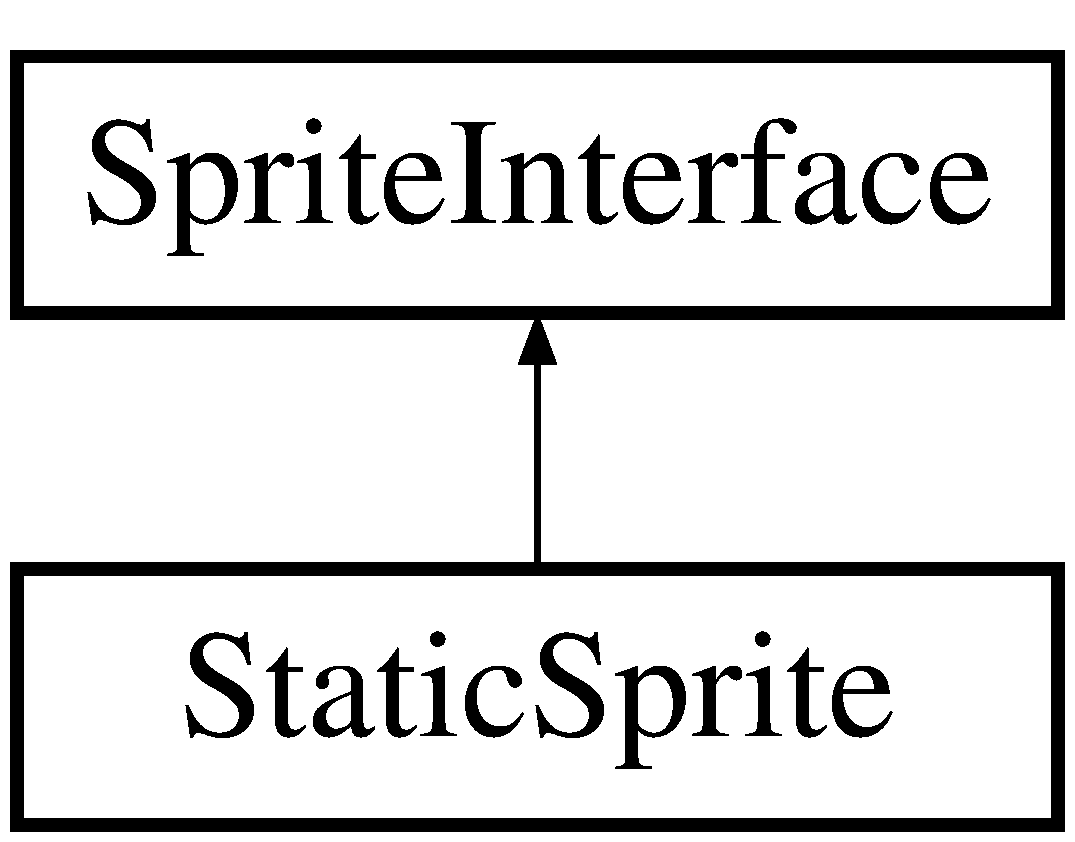
\includegraphics[height=2.000000cm]{class_static_sprite}
\end{center}
\end{figure}
\subsection*{Public Member Functions}
\begin{DoxyCompactItemize}
\item 
\mbox{\Hypertarget{class_static_sprite_ace8020b94a9aad1c7ac9928de6a1e495}\label{class_static_sprite_ace8020b94a9aad1c7ac9928de6a1e495}} 
\mbox{\hyperlink{class_static_sprite_ace8020b94a9aad1c7ac9928de6a1e495}{Static\+Sprite}} (int p\+\_\+col, int p\+\_\+row, sf\+::\+Texture p\+\_\+T, float p\+\_\+speed, float p\+\_\+health, float p\+\_\+damage)
\begin{DoxyCompactList}\small\item\em Constructor. \end{DoxyCompactList}\item 
\mbox{\hyperlink{class_static_sprite_a5e46df96b9b6660764f2b68b82109efc}{$\sim$\+Static\+Sprite}} ()
\begin{DoxyCompactList}\small\item\em Deconstructor. \end{DoxyCompactList}\item 
\mbox{\Hypertarget{class_static_sprite_a2dd0c3a98082f45d0d77d53d1af13b90}\label{class_static_sprite_a2dd0c3a98082f45d0d77d53d1af13b90}} 
void \mbox{\hyperlink{class_static_sprite_a2dd0c3a98082f45d0d77d53d1af13b90}{update}} (float p\+\_\+time) override
\begin{DoxyCompactList}\small\item\em update method \end{DoxyCompactList}\item 
void \mbox{\hyperlink{class_static_sprite_afe24127ebfb8a93de80fb42729a5f249}{message}} (const std\+::string p\+\_\+message) override
\begin{DoxyCompactList}\small\item\em message method \end{DoxyCompactList}\item 
sf\+::\+Sprite $\ast$ \mbox{\hyperlink{class_static_sprite_a516a9a18b60573cd0b3a5fd6199be0b9}{get\+Sprite}} () override
\begin{DoxyCompactList}\small\item\em gets the sprite \end{DoxyCompactList}\item 
\mbox{\Hypertarget{class_static_sprite_add5e0038c152e9d7e65afd47ba36abce}\label{class_static_sprite_add5e0038c152e9d7e65afd47ba36abce}} 
void \mbox{\hyperlink{class_static_sprite_add5e0038c152e9d7e65afd47ba36abce}{set\+Sprite\+Pos}} (int p\+\_\+col, int p\+\_\+row) override
\begin{DoxyCompactList}\small\item\em sets the pos of the sprite \end{DoxyCompactList}\item 
void \mbox{\hyperlink{class_static_sprite_a39f0883a2c8933804ab6bd172cdc02fd}{set\+Node}} (\mbox{\hyperlink{class_node_interface}{Node\+Interface}} $\ast$p\+\_\+\+NI) override
\begin{DoxyCompactList}\small\item\em set node \end{DoxyCompactList}\item 
\mbox{\hyperlink{class_node_interface}{Node\+Interface}} $\ast$ \mbox{\hyperlink{class_static_sprite_a672bb6e3425bbc15cd9034ab9e2802fd}{get\+Node}} () override
\begin{DoxyCompactList}\small\item\em get node \end{DoxyCompactList}\item 
\mbox{\Hypertarget{class_static_sprite_a975babf5d18d76c800a72a416558d7a4}\label{class_static_sprite_a975babf5d18d76c800a72a416558d7a4}} 
void \mbox{\hyperlink{class_static_sprite_a975babf5d18d76c800a72a416558d7a4}{set\+Health}} (float p\+\_\+damage\+Taken) override
\begin{DoxyCompactList}\small\item\em set health \end{DoxyCompactList}\item 
bool \mbox{\hyperlink{class_static_sprite_a4b037abeff328dd42777875fd145aae3}{is\+Doing\+Damage}} () override
\begin{DoxyCompactList}\small\item\em is it doing damage \end{DoxyCompactList}\item 
\mbox{\Hypertarget{class_static_sprite_a9b37e143ababf2b27a8372ab09f14f7b}\label{class_static_sprite_a9b37e143ababf2b27a8372ab09f14f7b}} 
void \mbox{\hyperlink{class_static_sprite_a9b37e143ababf2b27a8372ab09f14f7b}{do\+Damage}} (bool p\+\_\+bool) override
\begin{DoxyCompactList}\small\item\em Do damage. \end{DoxyCompactList}\end{DoxyCompactItemize}
\subsection*{Additional Inherited Members}


\subsection{Detailed Description}
This class builds up a character in the game 

\subsection{Constructor \& Destructor Documentation}
\mbox{\Hypertarget{class_static_sprite_a5e46df96b9b6660764f2b68b82109efc}\label{class_static_sprite_a5e46df96b9b6660764f2b68b82109efc}} 
\index{Static\+Sprite@{Static\+Sprite}!````~Static\+Sprite@{$\sim$\+Static\+Sprite}}
\index{````~Static\+Sprite@{$\sim$\+Static\+Sprite}!Static\+Sprite@{Static\+Sprite}}
\subsubsection{\texorpdfstring{$\sim$\+Static\+Sprite()}{~StaticSprite()}}
{\footnotesize\ttfamily Static\+Sprite\+::$\sim$\+Static\+Sprite (\begin{DoxyParamCaption}{ }\end{DoxyParamCaption})}



Deconstructor. 


\begin{DoxyParams}{Parameters}
{\em p\+\_\+col} & the column the sprite is on \\
\hline
{\em p\+\_\+row} & the row the sprite is on \\
\hline
{\em p\+\_\+t} & sprite texture \\
\hline
{\em p\+\_\+health} & the sprites health \\
\hline
{\em p\+\_\+damage} & the damage the sprite can do \\
\hline
\end{DoxyParams}


\subsection{Member Function Documentation}
\mbox{\Hypertarget{class_static_sprite_a672bb6e3425bbc15cd9034ab9e2802fd}\label{class_static_sprite_a672bb6e3425bbc15cd9034ab9e2802fd}} 
\index{Static\+Sprite@{Static\+Sprite}!get\+Node@{get\+Node}}
\index{get\+Node@{get\+Node}!Static\+Sprite@{Static\+Sprite}}
\subsubsection{\texorpdfstring{get\+Node()}{getNode()}}
{\footnotesize\ttfamily \mbox{\hyperlink{class_node_interface}{Node\+Interface}}$\ast$ Static\+Sprite\+::get\+Node (\begin{DoxyParamCaption}{ }\end{DoxyParamCaption})\hspace{0.3cm}{\ttfamily [override]}, {\ttfamily [virtual]}}



get node 


\begin{DoxyParams}{Parameters}
{\em p\+\_\+\+NI} & this node will become m\+\_\+node \\
\hline
\end{DoxyParams}


Reimplemented from \mbox{\hyperlink{class_sprite_interface_a0cda548d74975cb3dd3f4d163a1763b6}{Sprite\+Interface}}.

\mbox{\Hypertarget{class_static_sprite_a516a9a18b60573cd0b3a5fd6199be0b9}\label{class_static_sprite_a516a9a18b60573cd0b3a5fd6199be0b9}} 
\index{Static\+Sprite@{Static\+Sprite}!get\+Sprite@{get\+Sprite}}
\index{get\+Sprite@{get\+Sprite}!Static\+Sprite@{Static\+Sprite}}
\subsubsection{\texorpdfstring{get\+Sprite()}{getSprite()}}
{\footnotesize\ttfamily sf\+::\+Sprite$\ast$ Static\+Sprite\+::get\+Sprite (\begin{DoxyParamCaption}{ }\end{DoxyParamCaption})\hspace{0.3cm}{\ttfamily [override]}, {\ttfamily [virtual]}}



gets the sprite 


\begin{DoxyParams}{Parameters}
{\em p\+\_\+message} & its a message to the class \\
\hline
\end{DoxyParams}


Reimplemented from \mbox{\hyperlink{class_sprite_interface}{Sprite\+Interface}}.

\mbox{\Hypertarget{class_static_sprite_a4b037abeff328dd42777875fd145aae3}\label{class_static_sprite_a4b037abeff328dd42777875fd145aae3}} 
\index{Static\+Sprite@{Static\+Sprite}!is\+Doing\+Damage@{is\+Doing\+Damage}}
\index{is\+Doing\+Damage@{is\+Doing\+Damage}!Static\+Sprite@{Static\+Sprite}}
\subsubsection{\texorpdfstring{is\+Doing\+Damage()}{isDoingDamage()}}
{\footnotesize\ttfamily bool Static\+Sprite\+::is\+Doing\+Damage (\begin{DoxyParamCaption}{ }\end{DoxyParamCaption})\hspace{0.3cm}{\ttfamily [override]}, {\ttfamily [virtual]}}



is it doing damage 


\begin{DoxyParams}{Parameters}
{\em p\+\_\+damage} & taken subtracted from health \\
\hline
\end{DoxyParams}


Implements \mbox{\hyperlink{class_sprite_interface_a91a747b887e19cfc6e5256d4afc2f64c}{Sprite\+Interface}}.

\mbox{\Hypertarget{class_static_sprite_afe24127ebfb8a93de80fb42729a5f249}\label{class_static_sprite_afe24127ebfb8a93de80fb42729a5f249}} 
\index{Static\+Sprite@{Static\+Sprite}!message@{message}}
\index{message@{message}!Static\+Sprite@{Static\+Sprite}}
\subsubsection{\texorpdfstring{message()}{message()}}
{\footnotesize\ttfamily void Static\+Sprite\+::message (\begin{DoxyParamCaption}\item[{const std\+::string}]{p\+\_\+message }\end{DoxyParamCaption})\hspace{0.3cm}{\ttfamily [override]}, {\ttfamily [virtual]}}



message method 


\begin{DoxyParams}{Parameters}
{\em p\+\_\+time} & contains information on the time \\
\hline
\end{DoxyParams}


Implements \mbox{\hyperlink{class_sprite_interface_ad5335c5370f97cd81a52769cb0a25559}{Sprite\+Interface}}.

\mbox{\Hypertarget{class_static_sprite_a39f0883a2c8933804ab6bd172cdc02fd}\label{class_static_sprite_a39f0883a2c8933804ab6bd172cdc02fd}} 
\index{Static\+Sprite@{Static\+Sprite}!set\+Node@{set\+Node}}
\index{set\+Node@{set\+Node}!Static\+Sprite@{Static\+Sprite}}
\subsubsection{\texorpdfstring{set\+Node()}{setNode()}}
{\footnotesize\ttfamily void Static\+Sprite\+::set\+Node (\begin{DoxyParamCaption}\item[{\mbox{\hyperlink{class_node_interface}{Node\+Interface}} $\ast$}]{p\+\_\+\+NI }\end{DoxyParamCaption})\hspace{0.3cm}{\ttfamily [override]}, {\ttfamily [virtual]}}



set node 


\begin{DoxyParams}{Parameters}
{\em p\+\_\+row} & sets the row its in \\
\hline
{\em p\+\_\+col} & used to set what col its in \\
\hline
\end{DoxyParams}


Reimplemented from \mbox{\hyperlink{class_sprite_interface_aab826769df1222d5dd2ff426c8551bb2}{Sprite\+Interface}}.



The documentation for this class was generated from the following file\+:\begin{DoxyCompactItemize}
\item 
C\+:/\+Users/\+The Stormtrooper/\+Source/\+Repos/\+Final\+Year\+Project9/\+Vampires\+Vs\+Knights/include/Static\+Sprite.\+h\end{DoxyCompactItemize}

\hypertarget{class_texture_handler}{}\section{Texture\+Handler Class Reference}
\label{class_texture_handler}\index{Texture\+Handler@{Texture\+Handler}}


{\ttfamily \#include $<$Texture\+Handler.\+h$>$}

\subsection*{Public Member Functions}
\begin{DoxyCompactItemize}
\item 
\mbox{\Hypertarget{class_texture_handler_a6c6cfe48db6e9b582bc29b44c37758e6}\label{class_texture_handler_a6c6cfe48db6e9b582bc29b44c37758e6}} 
\mbox{\hyperlink{class_texture_handler_a6c6cfe48db6e9b582bc29b44c37758e6}{$\sim$\+Texture\+Handler}} ()
\begin{DoxyCompactList}\small\item\em Deconstructor. \end{DoxyCompactList}\item 
\mbox{\Hypertarget{class_texture_handler_ae3c5e0e1c61458009817ea91d4aa6eec}\label{class_texture_handler_ae3c5e0e1c61458009817ea91d4aa6eec}} 
void \mbox{\hyperlink{class_texture_handler_ae3c5e0e1c61458009817ea91d4aa6eec}{insert\+Texture}} (string p\+\_\+\+Path, string p\+\_\+\+Filename)
\begin{DoxyCompactList}\small\item\em add a texture \end{DoxyCompactList}\item 
sf\+::\+Texture \mbox{\hyperlink{class_texture_handler_a14f9286e41340937add40ec11453b2b4}{get\+Texture}} (string p\+\_\+\+File\+Name)
\begin{DoxyCompactList}\small\item\em get me the texture \end{DoxyCompactList}\item 
\mbox{\hyperlink{class_texture_handler_a1e980f198f0f1ec4bea0f670d8f72e88}{Texture\+Handler}} (\mbox{\hyperlink{class_texture_handler}{Texture\+Handler}} const \&)=delete
\begin{DoxyCompactList}\small\item\em Deletes the assigment operator. \end{DoxyCompactList}\item 
\mbox{\Hypertarget{class_texture_handler_adb37fce7620b391fd3ee6b1c2d8596e5}\label{class_texture_handler_adb37fce7620b391fd3ee6b1c2d8596e5}} 
\mbox{\hyperlink{class_texture_handler}{Texture\+Handler}} \& \mbox{\hyperlink{class_texture_handler_adb37fce7620b391fd3ee6b1c2d8596e5}{operator=}} (\mbox{\hyperlink{class_texture_handler}{Texture\+Handler}} const \&)=delete
\begin{DoxyCompactList}\small\item\em deletes the copy operator \end{DoxyCompactList}\end{DoxyCompactItemize}
\subsection*{Static Public Member Functions}
\begin{DoxyCompactItemize}
\item 
\mbox{\Hypertarget{class_texture_handler_a4f7833f068be40b04495c529bdbb8eb7}\label{class_texture_handler_a4f7833f068be40b04495c529bdbb8eb7}} 
static \mbox{\hyperlink{class_texture_handler}{Texture\+Handler}} $\ast$ \mbox{\hyperlink{class_texture_handler_a4f7833f068be40b04495c529bdbb8eb7}{instance}} ()
\begin{DoxyCompactList}\small\item\em calling the instance of the class \end{DoxyCompactList}\end{DoxyCompactItemize}
\subsection*{Private Member Functions}
\begin{DoxyCompactItemize}
\item 
\mbox{\Hypertarget{class_texture_handler_a9056de3d9a44b2e696c8e8b39462dd46}\label{class_texture_handler_a9056de3d9a44b2e696c8e8b39462dd46}} 
\mbox{\hyperlink{class_texture_handler_a9056de3d9a44b2e696c8e8b39462dd46}{Texture\+Handler}} ()
\begin{DoxyCompactList}\small\item\em Constructor. \end{DoxyCompactList}\end{DoxyCompactItemize}
\subsection*{Private Attributes}
\begin{DoxyCompactItemize}
\item 
\mbox{\Hypertarget{class_texture_handler_a65e3f9aa7333e9fd82259516f9c48c68}\label{class_texture_handler_a65e3f9aa7333e9fd82259516f9c48c68}} 
map$<$ string, sf\+::\+Texture $>$ \mbox{\hyperlink{class_texture_handler_a65e3f9aa7333e9fd82259516f9c48c68}{m\+\_\+map\+Of\+Textures}}
\begin{DoxyCompactList}\small\item\em Map holding textures. \end{DoxyCompactList}\item 
\mbox{\Hypertarget{class_texture_handler_a5449a61c7307806056cdb7dbfc3b8889}\label{class_texture_handler_a5449a61c7307806056cdb7dbfc3b8889}} 
std\+::vector$<$ std\+::string $>$ \mbox{\hyperlink{class_texture_handler_a5449a61c7307806056cdb7dbfc3b8889}{I\+Ds}}
\begin{DoxyCompactList}\small\item\em A vector containing the ID\textquotesingle{}s of the strings. \end{DoxyCompactList}\end{DoxyCompactItemize}
\subsection*{Static Private Attributes}
\begin{DoxyCompactItemize}
\item 
\mbox{\Hypertarget{class_texture_handler_af6548c4fd46c81523e63854ec4a54d01}\label{class_texture_handler_af6548c4fd46c81523e63854ec4a54d01}} 
static \mbox{\hyperlink{class_texture_handler}{Texture\+Handler}} $\ast$ \mbox{\hyperlink{class_texture_handler_af6548c4fd46c81523e63854ec4a54d01}{s\+\_\+\+Instance}}
\begin{DoxyCompactList}\small\item\em Create a instance of this. \end{DoxyCompactList}\end{DoxyCompactItemize}


\subsection{Detailed Description}
Singleton that handles all the textures in the game making it possible to get a texture whenever is needed 

\subsection{Constructor \& Destructor Documentation}
\mbox{\Hypertarget{class_texture_handler_a1e980f198f0f1ec4bea0f670d8f72e88}\label{class_texture_handler_a1e980f198f0f1ec4bea0f670d8f72e88}} 
\index{Texture\+Handler@{Texture\+Handler}!Texture\+Handler@{Texture\+Handler}}
\index{Texture\+Handler@{Texture\+Handler}!Texture\+Handler@{Texture\+Handler}}
\subsubsection{\texorpdfstring{Texture\+Handler()}{TextureHandler()}}
{\footnotesize\ttfamily Texture\+Handler\+::\+Texture\+Handler (\begin{DoxyParamCaption}\item[{\mbox{\hyperlink{class_texture_handler}{Texture\+Handler}} const \&}]{ }\end{DoxyParamCaption})\hspace{0.3cm}{\ttfamily [delete]}}



Deletes the assigment operator. 


\begin{DoxyParams}{Parameters}
{\em p\+\_\+\+File\+Name} & the name of the file \\
\hline
\end{DoxyParams}


\subsection{Member Function Documentation}
\mbox{\Hypertarget{class_texture_handler_a14f9286e41340937add40ec11453b2b4}\label{class_texture_handler_a14f9286e41340937add40ec11453b2b4}} 
\index{Texture\+Handler@{Texture\+Handler}!get\+Texture@{get\+Texture}}
\index{get\+Texture@{get\+Texture}!Texture\+Handler@{Texture\+Handler}}
\subsubsection{\texorpdfstring{get\+Texture()}{getTexture()}}
{\footnotesize\ttfamily sf\+::\+Texture Texture\+Handler\+::get\+Texture (\begin{DoxyParamCaption}\item[{string}]{p\+\_\+\+File\+Name }\end{DoxyParamCaption})}



get me the texture 


\begin{DoxyParams}{Parameters}
{\em p\+\_\+\+Path} & to get the texture \\
\hline
{\em p\+\_\+\+Filename} & name of the file \\
\hline
\end{DoxyParams}


The documentation for this class was generated from the following file\+:\begin{DoxyCompactItemize}
\item 
C\+:/\+Users/\+The Stormtrooper/\+Source/\+Repos/\+Final\+Year\+Project9/\+Vampires\+Vs\+Knights/include/Texture\+Handler.\+h\end{DoxyCompactItemize}

%--- End generated contents ---

% Index
\backmatter
\newpage
\phantomsection
\clearemptydoublepage
\addcontentsline{toc}{chapter}{Index}
\printindex

\end{document}
